% Options for packages loaded elsewhere
\PassOptionsToPackage{unicode}{hyperref}
\PassOptionsToPackage{hyphens}{url}
%
\documentclass[
]{book}
\usepackage{amsmath,amssymb}
\usepackage{lmodern}
\usepackage{iftex}
\ifPDFTeX
  \usepackage[T1]{fontenc}
  \usepackage[utf8]{inputenc}
  \usepackage{textcomp} % provide euro and other symbols
\else % if luatex or xetex
  \usepackage{unicode-math}
  \defaultfontfeatures{Scale=MatchLowercase}
  \defaultfontfeatures[\rmfamily]{Ligatures=TeX,Scale=1}
\fi
% Use upquote if available, for straight quotes in verbatim environments
\IfFileExists{upquote.sty}{\usepackage{upquote}}{}
\IfFileExists{microtype.sty}{% use microtype if available
  \usepackage[]{microtype}
  \UseMicrotypeSet[protrusion]{basicmath} % disable protrusion for tt fonts
}{}
\makeatletter
\@ifundefined{KOMAClassName}{% if non-KOMA class
  \IfFileExists{parskip.sty}{%
    \usepackage{parskip}
  }{% else
    \setlength{\parindent}{0pt}
    \setlength{\parskip}{6pt plus 2pt minus 1pt}}
}{% if KOMA class
  \KOMAoptions{parskip=half}}
\makeatother
\usepackage{xcolor}
\IfFileExists{xurl.sty}{\usepackage{xurl}}{} % add URL line breaks if available
\IfFileExists{bookmark.sty}{\usepackage{bookmark}}{\usepackage{hyperref}}
\hypersetup{
  pdftitle={Python and R},
  pdfauthor={Clay Ford, Jacob Goldstein-Greenwood, Oyinkansola Adenekan, Samantha Lomuscio},
  hidelinks,
  pdfcreator={LaTeX via pandoc}}
\urlstyle{same} % disable monospaced font for URLs
\usepackage{color}
\usepackage{fancyvrb}
\newcommand{\VerbBar}{|}
\newcommand{\VERB}{\Verb[commandchars=\\\{\}]}
\DefineVerbatimEnvironment{Highlighting}{Verbatim}{commandchars=\\\{\}}
% Add ',fontsize=\small' for more characters per line
\usepackage{framed}
\definecolor{shadecolor}{RGB}{248,248,248}
\newenvironment{Shaded}{\begin{snugshade}}{\end{snugshade}}
\newcommand{\AlertTok}[1]{\textcolor[rgb]{0.94,0.16,0.16}{#1}}
\newcommand{\AnnotationTok}[1]{\textcolor[rgb]{0.56,0.35,0.01}{\textbf{\textit{#1}}}}
\newcommand{\AttributeTok}[1]{\textcolor[rgb]{0.77,0.63,0.00}{#1}}
\newcommand{\BaseNTok}[1]{\textcolor[rgb]{0.00,0.00,0.81}{#1}}
\newcommand{\BuiltInTok}[1]{#1}
\newcommand{\CharTok}[1]{\textcolor[rgb]{0.31,0.60,0.02}{#1}}
\newcommand{\CommentTok}[1]{\textcolor[rgb]{0.56,0.35,0.01}{\textit{#1}}}
\newcommand{\CommentVarTok}[1]{\textcolor[rgb]{0.56,0.35,0.01}{\textbf{\textit{#1}}}}
\newcommand{\ConstantTok}[1]{\textcolor[rgb]{0.00,0.00,0.00}{#1}}
\newcommand{\ControlFlowTok}[1]{\textcolor[rgb]{0.13,0.29,0.53}{\textbf{#1}}}
\newcommand{\DataTypeTok}[1]{\textcolor[rgb]{0.13,0.29,0.53}{#1}}
\newcommand{\DecValTok}[1]{\textcolor[rgb]{0.00,0.00,0.81}{#1}}
\newcommand{\DocumentationTok}[1]{\textcolor[rgb]{0.56,0.35,0.01}{\textbf{\textit{#1}}}}
\newcommand{\ErrorTok}[1]{\textcolor[rgb]{0.64,0.00,0.00}{\textbf{#1}}}
\newcommand{\ExtensionTok}[1]{#1}
\newcommand{\FloatTok}[1]{\textcolor[rgb]{0.00,0.00,0.81}{#1}}
\newcommand{\FunctionTok}[1]{\textcolor[rgb]{0.00,0.00,0.00}{#1}}
\newcommand{\ImportTok}[1]{#1}
\newcommand{\InformationTok}[1]{\textcolor[rgb]{0.56,0.35,0.01}{\textbf{\textit{#1}}}}
\newcommand{\KeywordTok}[1]{\textcolor[rgb]{0.13,0.29,0.53}{\textbf{#1}}}
\newcommand{\NormalTok}[1]{#1}
\newcommand{\OperatorTok}[1]{\textcolor[rgb]{0.81,0.36,0.00}{\textbf{#1}}}
\newcommand{\OtherTok}[1]{\textcolor[rgb]{0.56,0.35,0.01}{#1}}
\newcommand{\PreprocessorTok}[1]{\textcolor[rgb]{0.56,0.35,0.01}{\textit{#1}}}
\newcommand{\RegionMarkerTok}[1]{#1}
\newcommand{\SpecialCharTok}[1]{\textcolor[rgb]{0.00,0.00,0.00}{#1}}
\newcommand{\SpecialStringTok}[1]{\textcolor[rgb]{0.31,0.60,0.02}{#1}}
\newcommand{\StringTok}[1]{\textcolor[rgb]{0.31,0.60,0.02}{#1}}
\newcommand{\VariableTok}[1]{\textcolor[rgb]{0.00,0.00,0.00}{#1}}
\newcommand{\VerbatimStringTok}[1]{\textcolor[rgb]{0.31,0.60,0.02}{#1}}
\newcommand{\WarningTok}[1]{\textcolor[rgb]{0.56,0.35,0.01}{\textbf{\textit{#1}}}}
\usepackage{longtable,booktabs,array}
\usepackage{calc} % for calculating minipage widths
% Correct order of tables after \paragraph or \subparagraph
\usepackage{etoolbox}
\makeatletter
\patchcmd\longtable{\par}{\if@noskipsec\mbox{}\fi\par}{}{}
\makeatother
% Allow footnotes in longtable head/foot
\IfFileExists{footnotehyper.sty}{\usepackage{footnotehyper}}{\usepackage{footnote}}
\makesavenoteenv{longtable}
\usepackage{graphicx}
\makeatletter
\def\maxwidth{\ifdim\Gin@nat@width>\linewidth\linewidth\else\Gin@nat@width\fi}
\def\maxheight{\ifdim\Gin@nat@height>\textheight\textheight\else\Gin@nat@height\fi}
\makeatother
% Scale images if necessary, so that they will not overflow the page
% margins by default, and it is still possible to overwrite the defaults
% using explicit options in \includegraphics[width, height, ...]{}
\setkeys{Gin}{width=\maxwidth,height=\maxheight,keepaspectratio}
% Set default figure placement to htbp
\makeatletter
\def\fps@figure{htbp}
\makeatother
\setlength{\emergencystretch}{3em} % prevent overfull lines
\providecommand{\tightlist}{%
  \setlength{\itemsep}{0pt}\setlength{\parskip}{0pt}}
\setcounter{secnumdepth}{5}
\usepackage{booktabs}
\ifLuaTeX
  \usepackage{selnolig}  % disable illegal ligatures
\fi
\usepackage[]{natbib}
\bibliographystyle{plainnat}
\nocite{*}

\title{Python and R}
\author{Clay Ford, Jacob Goldstein-Greenwood, Oyinkansola Adenekan, Samantha Lomuscio}
\date{2021-10-26}

\begin{document}
\maketitle

{
\setcounter{tocdepth}{1}
\tableofcontents
}
\hypertarget{welcome}{%
\chapter*{Welcome}\label{welcome}}
\addcontentsline{toc}{chapter}{Welcome}

This book provides parallel examples in Python and R to help users of one platform more easily learn how the other platform ``works'' when it comes to data analysis.

\hypertarget{basics}{%
\chapter{Basics}\label{basics}}

This chapter covers the very basics of Python and R.

\hypertarget{math}{%
\section{Math}\label{math}}

Mathematical operators are the same except for exponents, integer division, and remainder division (modulo).

\hypertarget{python} for remainder division.

\begin{Shaded}
\begin{Highlighting}[]
\OperatorTok{\textgreater{}} \DecValTok{3}\OperatorTok{**}\DecValTok{2}
\DecValTok{9}
\OperatorTok{\textgreater{}} \DecValTok{5} \OperatorTok{//} \DecValTok{2}
\DecValTok{2}
\OperatorTok{\textgreater{}} \DecValTok{5} \OperatorTok{\%} \DecValTok{2}
\DecValTok{1}
\end{Highlighting}
\end{Shaded}

In Python, the \texttt{+} operator can also be used to combine strings. See this TBD section.

\hypertarget{r}{%
\subsubsection*{R}\label{r}}
\addcontentsline{toc}{subsubsection}{R}

Python uses \texttt{\^{}} for exponentiation, \texttt{\%/\%} for integer division, and \texttt{\%\%} for remainder division.

\begin{Shaded}
\begin{Highlighting}[]
\SpecialCharTok{\textgreater{}} \DecValTok{3}\SpecialCharTok{\^{}}\DecValTok{2}
\NormalTok{[}\DecValTok{1}\NormalTok{] }\DecValTok{9}
\SpecialCharTok{\textgreater{}} \DecValTok{5} \SpecialCharTok{\%/\%} \DecValTok{2}
\NormalTok{[}\DecValTok{1}\NormalTok{] }\DecValTok{2}
\SpecialCharTok{\textgreater{}} \DecValTok{5} \SpecialCharTok{\%\%} \DecValTok{2}
\NormalTok{[}\DecValTok{1}\NormalTok{] }\DecValTok{1}
\end{Highlighting}
\end{Shaded}

\hypertarget{assignment}{%
\section{Assignment}\label{assignment}}

Python uses \texttt{=} for assignment while R can use either \texttt{=} or \texttt{\textless{}-} for assignment. The latter ``assignment arrow'' is preferred in most R style guides to distinguish it between assignment and setting the value of a function argument. According to R's documentation, ``The operator \texttt{\textless{}-} can be used anywhere, whereas the operator \texttt{=} is only allowed at the top level (e.g., in the complete expression typed at the command prompt) or as one of the subexpressions in a braced list of expressions.'' See \texttt{?assignOps}.

\hypertarget{python-1}{%
\subsubsection*{Python}\label{python-1}}
\addcontentsline{toc}{subsubsection}{Python}

\begin{Shaded}
\begin{Highlighting}[]
\OperatorTok{\textgreater{}}\NormalTok{ x }\OperatorTok{=} \DecValTok{12}
\end{Highlighting}
\end{Shaded}

\hypertarget{r-1}{%
\subsubsection*{R}\label{r-1}}
\addcontentsline{toc}{subsubsection}{R}

\begin{Shaded}
\begin{Highlighting}[]
\SpecialCharTok{\textgreater{}}\NormalTok{ x }\OtherTok{\textless{}{-}} \DecValTok{12}
\end{Highlighting}
\end{Shaded}

\hypertarget{printing-a-value}{%
\section{Printing a value}\label{printing-a-value}}

To see the value of an object created via assignment, you can simply enter the object at the console and hit enter for both Python and R, though it is common in Python to explicitly use the \texttt{print()} function.

\hypertarget{python-2}{%
\subsubsection*{Python}\label{python-2}}
\addcontentsline{toc}{subsubsection}{Python}

\begin{Shaded}
\begin{Highlighting}[]
\OperatorTok{\textgreater{}}\NormalTok{ x}
\DecValTok{12}
\end{Highlighting}
\end{Shaded}

\hypertarget{r-2}{%
\subsubsection*{R}\label{r-2}}
\addcontentsline{toc}{subsubsection}{R}

\begin{Shaded}
\begin{Highlighting}[]
\SpecialCharTok{\textgreater{}}\NormalTok{ x}
\NormalTok{[}\DecValTok{1}\NormalTok{] }\DecValTok{12}
\end{Highlighting}
\end{Shaded}

\hypertarget{packages}{%
\section{Packages}\label{packages}}

User-created functions can be bundled and distributed as packages. Packages need to be installed only once. Thereafter they're ``imported'' (Python) or ``loaded'' (R) in each new session when needed.

Packages with large user bases are often updated to add functionality and fix bugs. The updates are not automatically installed. Staying apprised of library/package updates can be challenging. Some suggestions are following developers on Twitter, signing up for newsletters, or periodically checking to see what updates are available.

Packages often depend on other packages. These are known as ``dependencies.'' Sometimes packages are updated to accommodate changes to other packages they depend on.

\hypertarget{python-3}{%
\subsubsection*{Python}\label{python-3}}
\addcontentsline{toc}{subsubsection}{Python}

\hypertarget{r-3}{%
\subsubsection*{R}\label{r-3}}
\addcontentsline{toc}{subsubsection}{R}

The main repository for R packages is the \href{https://cran.r-project.org/}{Comprehensive R Archive Network} (CRAN). Another repository is \href{https://www.bioconductor.org/}{Bioconductor}, which provides tools for working with genomic data. Many packages are also distributed on \href{https://github.com/}{GitHub}.

To install packages from CRAN use the \texttt{install.packages()} function. In RStudio, you can also go to Tools\ldots Install Packages\ldots{} for a dialog that will auto-complete package names as you type.

\begin{Shaded}
\begin{Highlighting}[]
\SpecialCharTok{\textgreater{}} \CommentTok{\# install the vcd package, a package for Visualizing Categorical Data}
\ErrorTok{\textgreater{}} \FunctionTok{install.packages}\NormalTok{(}\StringTok{"vcd"}\NormalTok{)}
\SpecialCharTok{\textgreater{}} 
\ErrorTok{\textgreater{}} \CommentTok{\# load the package}
\ErrorTok{\textgreater{}} \FunctionTok{library}\NormalTok{(vcd)}
\SpecialCharTok{\textgreater{}} 
\ErrorTok{\textgreater{}} \CommentTok{\# see which packages on your computer have updates available}
\ErrorTok{\textgreater{}} \FunctionTok{old.packages}\NormalTok{()}
\SpecialCharTok{\textgreater{}} 
\ErrorTok{\textgreater{}} \CommentTok{\# download and install available package updates;}
\ErrorTok{\textgreater{}} \CommentTok{\# set ask = TRUE to verify installation of each package}
\ErrorTok{\textgreater{}} \FunctionTok{update.packages}\NormalTok{(}\AttributeTok{ask =} \ConstantTok{FALSE}\NormalTok{)}
\end{Highlighting}
\end{Shaded}

To install R packages from GitHub use the \texttt{install\_github()} function from the \textbf{devtools} package. You need to include the username of the repo owner followed by a forward slash and the name of the package. Typing two colons between a package and a function in the package allows you to use that function without loading the package. That's how we use the \texttt{install\_github()} below.

\begin{Shaded}
\begin{Highlighting}[]
\SpecialCharTok{\textgreater{}} \FunctionTok{install.packages}\NormalTok{(}\StringTok{"devtools"}\NormalTok{)}
\SpecialCharTok{\textgreater{}}\NormalTok{ devtools}\SpecialCharTok{::}\FunctionTok{install\_github}\NormalTok{(}\StringTok{"username/packagename"}\NormalTok{)}
\end{Highlighting}
\end{Shaded}

Occasionally when installing package updates you will be asked ``Do you want to install from sources the package which needs compilation?'' R packages on CRAN are \emph{compiled} for Mac and Windows operating systems. That can take a day or two after a package has been submitted to CRAN. If you try to install a package that has not been compiled then you'll get asked the question above. If you click \emph{Yes}, R will try to compile the package on your computer. This will only work if you have the required build tools on your computer. For Windows this means having \href{https://cran.r-project.org/bin/windows/Rtools/}{Rtools} installed. Mac users should already have the necessary build tools. Unless you absolutely need the latest version of a package, it's probably fine to click \emph{No}.

\hypertarget{logic}{%
\section{Logic}\label{logic}}

Python and R share the same operators for making comparisons:

\begin{itemize}
\tightlist
\item
  \texttt{==} (equals)
\item
  \texttt{!=} (not equal to)
\item
  \texttt{\textless{}} (less than)
\item
  \texttt{\textless{}=} (less than or equal to)
\item
  \texttt{\textgreater{}} (greater than)
\item
  \texttt{\textgreater{}=} (greater than or equal to)
\end{itemize}

Likewise they share the same operators for logical AND and OR:

\begin{itemize}
\tightlist
\item
  \texttt{\&} (AND)
\item
  \texttt{\textbar{}} (OR)
\end{itemize}

However R also has \texttt{\&\&} and \texttt{\textbar{}\textbar{}} operators for programming control-flow.

Python and R have different operators for negation and xor (exclusive OR).

\hypertarget{python-4}{%
\subsubsection*{Python}\label{python-4}}
\addcontentsline{toc}{subsubsection}{Python}

\hypertarget{r-4}{%
\subsubsection*{R}\label{r-4}}
\addcontentsline{toc}{subsubsection}{R}

\hypertarget{generating-a-sequence-of-values}{%
\section{Generating a sequence of values}\label{generating-a-sequence-of-values}}

In Python, one option for generating a sequence of values is \texttt{arange()} from \textbf{NumPy}. In R, a common approach is to use \texttt{seq()}. The sequences can be incremented by indicating a \texttt{step} argument in \texttt{arange()} or a \texttt{by} argument in \texttt{seq()}. Be aware that the end of the start/stop interval in \texttt{arange()} is \emph{open}, but both sides of the from/to interval in \texttt{seq()} are \emph{closed}.

\hypertarget{python-5}{%
\subsubsection*{Python}\label{python-5}}
\addcontentsline{toc}{subsubsection}{Python}

\begin{Shaded}
\begin{Highlighting}[]
\OperatorTok{\textgreater{}} \ImportTok{import}\NormalTok{ numpy }\ImportTok{as}\NormalTok{ np}
\OperatorTok{+}\NormalTok{ x }\OperatorTok{=}\NormalTok{ np.arange(start }\OperatorTok{=} \DecValTok{1}\NormalTok{, stop }\OperatorTok{=} \DecValTok{11}\NormalTok{, step }\OperatorTok{=} \DecValTok{2}\NormalTok{)}
\OperatorTok{+}\NormalTok{ x}
\NormalTok{array([}\DecValTok{1}\NormalTok{, }\DecValTok{3}\NormalTok{, }\DecValTok{5}\NormalTok{, }\DecValTok{7}\NormalTok{, }\DecValTok{9}\NormalTok{])}
\end{Highlighting}
\end{Shaded}

\hypertarget{r-5}{%
\subsubsection*{R}\label{r-5}}
\addcontentsline{toc}{subsubsection}{R}

\begin{Shaded}
\begin{Highlighting}[]
\SpecialCharTok{\textgreater{}}\NormalTok{ x }\OtherTok{\textless{}{-}} \FunctionTok{seq}\NormalTok{(}\AttributeTok{from =} \DecValTok{1}\NormalTok{, }\AttributeTok{to =} \DecValTok{11}\NormalTok{, }\AttributeTok{by =} \DecValTok{2}\NormalTok{)}
\SpecialCharTok{\textgreater{}}\NormalTok{ x}
\NormalTok{[}\DecValTok{1}\NormalTok{]  }\DecValTok{1}  \DecValTok{3}  \DecValTok{5}  \DecValTok{7}  \DecValTok{9} \DecValTok{11}
\end{Highlighting}
\end{Shaded}

\hypertarget{calculating-means-and-medians}{%
\section{Calculating means and medians}\label{calculating-means-and-medians}}

The \textbf{NumPy} Python library has functions for calculating means and medians, and base R has functions for doing the same.

\hypertarget{python-6}{%
\subsubsection*{Python}\label{python-6}}
\addcontentsline{toc}{subsubsection}{Python}

Mean, using function from \textbf{NumPy} library

\begin{Shaded}
\begin{Highlighting}[]
\OperatorTok{\textgreater{}} \ImportTok{import}\NormalTok{ numpy }\ImportTok{as}\NormalTok{ np}
\OperatorTok{+}\NormalTok{ x }\OperatorTok{=}\NormalTok{ [}\DecValTok{90}\NormalTok{, }\DecValTok{105}\NormalTok{, }\DecValTok{110}\NormalTok{]}
\OperatorTok{+}\NormalTok{ x\_avg }\OperatorTok{=}\NormalTok{ np.mean(x)}
\OperatorTok{+} \BuiltInTok{print}\NormalTok{(x\_avg)}
\FloatTok{101.66666666666667}
\end{Highlighting}
\end{Shaded}

Median, using function from \textbf{NumPy} library

\begin{Shaded}
\begin{Highlighting}[]
\OperatorTok{\textgreater{}}\NormalTok{ x }\OperatorTok{=}\NormalTok{ [}\DecValTok{98}\NormalTok{, }\DecValTok{102}\NormalTok{, }\DecValTok{20}\NormalTok{, }\DecValTok{22}\NormalTok{, }\DecValTok{304}\NormalTok{]}
\OperatorTok{+}\NormalTok{ x\_med }\OperatorTok{=}\NormalTok{ np.median(x)}
\OperatorTok{+} \BuiltInTok{print}\NormalTok{(x\_med)}
\FloatTok{98.0}
\end{Highlighting}
\end{Shaded}

\hypertarget{r-6}{%
\subsubsection*{R}\label{r-6}}
\addcontentsline{toc}{subsubsection}{R}

Mean, using function from base R

\begin{Shaded}
\begin{Highlighting}[]
\SpecialCharTok{\textgreater{}}\NormalTok{ x }\OtherTok{\textless{}{-}} \FunctionTok{c}\NormalTok{(}\DecValTok{90}\NormalTok{, }\DecValTok{105}\NormalTok{, }\DecValTok{110}\NormalTok{)}
\SpecialCharTok{\textgreater{}}\NormalTok{ x\_avg }\OtherTok{\textless{}{-}} \FunctionTok{mean}\NormalTok{(x)}
\SpecialCharTok{\textgreater{}}\NormalTok{ x\_avg}
\NormalTok{[}\DecValTok{1}\NormalTok{] }\FloatTok{101.6667}
\end{Highlighting}
\end{Shaded}

Median, using function from base R

\begin{Shaded}
\begin{Highlighting}[]
\SpecialCharTok{\textgreater{}}\NormalTok{ x }\OtherTok{\textless{}{-}} \FunctionTok{c}\NormalTok{(}\DecValTok{98}\NormalTok{, }\DecValTok{102}\NormalTok{, }\DecValTok{20}\NormalTok{, }\DecValTok{22}\NormalTok{, }\DecValTok{304}\NormalTok{)}
\SpecialCharTok{\textgreater{}}\NormalTok{ x\_med }\OtherTok{\textless{}{-}} \FunctionTok{median}\NormalTok{(x)}
\SpecialCharTok{\textgreater{}}\NormalTok{ x\_med}
\NormalTok{[}\DecValTok{1}\NormalTok{] }\DecValTok{98}
\end{Highlighting}
\end{Shaded}

\hypertarget{data-structures}{%
\chapter{Data Structures}\label{data-structures}}

This chapter compares and contrasts data structures in Python and R.

\hypertarget{one-dimensional-data}{%
\section{One-dimensional data}\label{one-dimensional-data}}

A one-dimensional data structure can be visualized as a column in a spreadsheet or as a list of values.

\hypertarget{python-7}{%
\subsubsection*{Python}\label{python-7}}
\addcontentsline{toc}{subsubsection}{Python}

\hypertarget{r-7}{%
\subsubsection*{R}\label{r-7}}
\addcontentsline{toc}{subsubsection}{R}

In R a one-dimensional data structure is called a \emph{vector}. We can create a vector using the \texttt{c()} function. A vector in R can only contain one type of data (all numbers, all strings, etc). The columns of data frames are vectors. If multiple types of data are put into a vector, the data will be coerced according to the hierarchy \texttt{logical} \textless{} \texttt{integer} \textless{} \texttt{double} \textless{} \texttt{complex} \textless{} \texttt{character}. This means if you mix, say, integers and character data, all the data will be coerced to character.

\begin{Shaded}
\begin{Highlighting}[]
\SpecialCharTok{\textgreater{}}\NormalTok{ x1 }\OtherTok{\textless{}{-}} \FunctionTok{c}\NormalTok{(}\DecValTok{23}\NormalTok{, }\DecValTok{43}\NormalTok{, }\DecValTok{55}\NormalTok{)}
\SpecialCharTok{\textgreater{}}\NormalTok{ x1}
\NormalTok{[}\DecValTok{1}\NormalTok{] }\DecValTok{23} \DecValTok{43} \DecValTok{55}
\SpecialCharTok{\textgreater{}} 
\ErrorTok{\textgreater{}} \CommentTok{\# all values coerced to character}
\ErrorTok{\textgreater{}}\NormalTok{ x2 }\OtherTok{\textless{}{-}} \FunctionTok{c}\NormalTok{(}\DecValTok{23}\NormalTok{, }\DecValTok{43}\NormalTok{, }\StringTok{\textquotesingle{}hi\textquotesingle{}}\NormalTok{)}
\SpecialCharTok{\textgreater{}}\NormalTok{ x2}
\NormalTok{[}\DecValTok{1}\NormalTok{] }\StringTok{"23"} \StringTok{"43"} \StringTok{"hi"}
\end{Highlighting}
\end{Shaded}

Values in a vector can be accessed by position using indexing brackets.

\begin{Shaded}
\begin{Highlighting}[]
\SpecialCharTok{\textgreater{}} \CommentTok{\# extract the 2nd value}
\ErrorTok{\textgreater{}}\NormalTok{ x1[}\DecValTok{2}\NormalTok{]}
\NormalTok{[}\DecValTok{1}\NormalTok{] }\DecValTok{43}
\SpecialCharTok{\textgreater{}} 
\ErrorTok{\textgreater{}} \CommentTok{\# extract the 2nd and 3rd value}
\ErrorTok{\textgreater{}}\NormalTok{ x1[}\DecValTok{2}\SpecialCharTok{:}\DecValTok{3}\NormalTok{]}
\NormalTok{[}\DecValTok{1}\NormalTok{] }\DecValTok{43} \DecValTok{55}
\end{Highlighting}
\end{Shaded}

\hypertarget{two-dimensional-data}{%
\section{Two-dimensional data}\label{two-dimensional-data}}

Two-dimensional data are rectangular in nature, consisting of rows and columns. These can be the type of data you might find in a spreadsheet with a mix of data types in columns; they can also be matrices as you might encounter in matrix algebra.

\hypertarget{python-8}{%
\subsubsection*{Python}\label{python-8}}
\addcontentsline{toc}{subsubsection}{Python}

\hypertarget{r-8}{%
\subsubsection*{R}\label{r-8}}
\addcontentsline{toc}{subsubsection}{R}

Two-dimensional data structures in R include the \emph{matrix} and \emph{data frame}. A matrix can contain only one data type. A data frame can contain multiple vectors each of which can consist of different data types.

Create a matrix with the \texttt{matrix()} function. Create a data frame with the \texttt{data.frame()} function. Most imported data comes into R as a data frame.

\begin{Shaded}
\begin{Highlighting}[]
\SpecialCharTok{\textgreater{}} \CommentTok{\# matrix; populated down by column by default}
\ErrorTok{\textgreater{}}\NormalTok{ m }\OtherTok{\textless{}{-}} \FunctionTok{matrix}\NormalTok{(}\AttributeTok{data =} \FunctionTok{c}\NormalTok{(}\DecValTok{1}\NormalTok{,}\DecValTok{3}\NormalTok{,}\DecValTok{5}\NormalTok{,}\DecValTok{7}\NormalTok{), }\AttributeTok{nrow =} \DecValTok{2}\NormalTok{, }\AttributeTok{ncol =} \DecValTok{2}\NormalTok{)}
\SpecialCharTok{\textgreater{}}\NormalTok{ m}
\NormalTok{     [,}\DecValTok{1}\NormalTok{] [,}\DecValTok{2}\NormalTok{]}
\NormalTok{[}\DecValTok{1}\NormalTok{,]    }\DecValTok{1}    \DecValTok{5}
\NormalTok{[}\DecValTok{2}\NormalTok{,]    }\DecValTok{3}    \DecValTok{7}
\SpecialCharTok{\textgreater{}} 
\ErrorTok{\textgreater{}} \CommentTok{\# data frame}
\ErrorTok{\textgreater{}}\NormalTok{ d }\OtherTok{\textless{}{-}} \FunctionTok{data.frame}\NormalTok{(}\AttributeTok{name =} \FunctionTok{c}\NormalTok{(}\StringTok{"Rob"}\NormalTok{, }\StringTok{"Cindy"}\NormalTok{),}
\SpecialCharTok{+}                 \AttributeTok{age =} \FunctionTok{c}\NormalTok{(}\DecValTok{35}\NormalTok{, }\DecValTok{37}\NormalTok{))}
\SpecialCharTok{\textgreater{}}\NormalTok{ d}
\NormalTok{   name age}
\DecValTok{1}\NormalTok{   Rob  }\DecValTok{35}
\DecValTok{2}\NormalTok{ Cindy  }\DecValTok{37}
\end{Highlighting}
\end{Shaded}

Values in a matrix and data frame can be accessed by position using indexing brackets. The first number(s) refers to rows; the second number(s) refers to columns. Leaving row or column numbers empty selects all rows or columns.

\begin{Shaded}
\begin{Highlighting}[]
\SpecialCharTok{\textgreater{}} \CommentTok{\# extract value in row 1, column 2}
\ErrorTok{\textgreater{}}\NormalTok{ m[}\DecValTok{1}\NormalTok{,}\DecValTok{2}\NormalTok{]}
\NormalTok{[}\DecValTok{1}\NormalTok{] }\DecValTok{5}
\SpecialCharTok{\textgreater{}} 
\ErrorTok{\textgreater{}} \CommentTok{\# extract values in row 2}
\ErrorTok{\textgreater{}}\NormalTok{ d[}\DecValTok{2}\NormalTok{,]}
\NormalTok{   name age}
\DecValTok{2}\NormalTok{ Cindy  }\DecValTok{37}
\end{Highlighting}
\end{Shaded}

\hypertarget{three-dimensional-and-higher-data}{%
\section{Three-dimensional and higher data}\label{three-dimensional-and-higher-data}}

Three-dimensional and higher data can be visualized as multiple rectangular structures stratified by extra variables. These are sometimes referred to as \emph{arrays}. Analysts usually prefer two-dimensional data frames to arrays. Data frames can accommodate multidimensional data by including the additional dimensions as variables.

\hypertarget{python-9}{%
\subsubsection*{Python}\label{python-9}}
\addcontentsline{toc}{subsubsection}{Python}

\hypertarget{r-9}{%
\subsubsection*{R}\label{r-9}}
\addcontentsline{toc}{subsubsection}{R}

The \texttt{array()} function in R can create three-dimensional and higher data structures. Specify the dimension number and size using the \texttt{dim} argument. Below we specify 2 rows, 3 columns, and 2 strata using a vector: \texttt{c(2,3,2)}. This creates a three-dimensional data structure. The data are simply the numbers 1 through 12.

\begin{Shaded}
\begin{Highlighting}[]
\SpecialCharTok{\textgreater{}}\NormalTok{ a1 }\OtherTok{\textless{}{-}} \FunctionTok{array}\NormalTok{(}\AttributeTok{data =} \DecValTok{1}\SpecialCharTok{:}\DecValTok{12}\NormalTok{, }\AttributeTok{dim =} \FunctionTok{c}\NormalTok{(}\DecValTok{2}\NormalTok{,}\DecValTok{3}\NormalTok{,}\DecValTok{2}\NormalTok{))}
\SpecialCharTok{\textgreater{}}\NormalTok{ a1}
\NormalTok{, , }\DecValTok{1}

\NormalTok{     [,}\DecValTok{1}\NormalTok{] [,}\DecValTok{2}\NormalTok{] [,}\DecValTok{3}\NormalTok{]}
\NormalTok{[}\DecValTok{1}\NormalTok{,]    }\DecValTok{1}    \DecValTok{3}    \DecValTok{5}
\NormalTok{[}\DecValTok{2}\NormalTok{,]    }\DecValTok{2}    \DecValTok{4}    \DecValTok{6}

\NormalTok{, , }\DecValTok{2}

\NormalTok{     [,}\DecValTok{1}\NormalTok{] [,}\DecValTok{2}\NormalTok{] [,}\DecValTok{3}\NormalTok{]}
\NormalTok{[}\DecValTok{1}\NormalTok{,]    }\DecValTok{7}    \DecValTok{9}   \DecValTok{11}
\NormalTok{[}\DecValTok{2}\NormalTok{,]    }\DecValTok{8}   \DecValTok{10}   \DecValTok{12}
\end{Highlighting}
\end{Shaded}

Values in arrays can be accessed by position using indexing brackets.

\begin{Shaded}
\begin{Highlighting}[]
\SpecialCharTok{\textgreater{}} \CommentTok{\# extract value in row 1, column 2, strata 1}
\ErrorTok{\textgreater{}}\NormalTok{ a1[}\DecValTok{1}\NormalTok{,}\DecValTok{2}\NormalTok{,}\DecValTok{1}\NormalTok{]}
\NormalTok{[}\DecValTok{1}\NormalTok{] }\DecValTok{3}
\SpecialCharTok{\textgreater{}} 
\ErrorTok{\textgreater{}} \CommentTok{\# extract column 2 in both strata}
\ErrorTok{\textgreater{}} \CommentTok{\# result is returned as matrix}
\ErrorTok{\textgreater{}}\NormalTok{ a1[,}\DecValTok{2}\NormalTok{,]}
\NormalTok{     [,}\DecValTok{1}\NormalTok{] [,}\DecValTok{2}\NormalTok{]}
\NormalTok{[}\DecValTok{1}\NormalTok{,]    }\DecValTok{3}    \DecValTok{9}
\NormalTok{[}\DecValTok{2}\NormalTok{,]    }\DecValTok{4}   \DecValTok{10}
\end{Highlighting}
\end{Shaded}

The dimensions can be named using the \texttt{dimnames()} function. Notice the names must be a \emph{list}.

\begin{Shaded}
\begin{Highlighting}[]
\SpecialCharTok{\textgreater{}} \FunctionTok{dimnames}\NormalTok{(a1) }\OtherTok{\textless{}{-}} \FunctionTok{list}\NormalTok{(}\StringTok{"X"} \OtherTok{=} \FunctionTok{c}\NormalTok{(}\StringTok{"x1"}\NormalTok{, }\StringTok{"x2"}\NormalTok{), }
\SpecialCharTok{+}                      \StringTok{"Y"} \OtherTok{=} \FunctionTok{c}\NormalTok{(}\StringTok{"y1"}\NormalTok{, }\StringTok{"y2"}\NormalTok{, }\StringTok{"y3"}\NormalTok{), }
\SpecialCharTok{+}                      \StringTok{"Z"} \OtherTok{=} \FunctionTok{c}\NormalTok{(}\StringTok{"z1"}\NormalTok{, }\StringTok{"z2"}\NormalTok{))}
\SpecialCharTok{\textgreater{}}\NormalTok{ a1}
\NormalTok{, , Z }\OtherTok{=}\NormalTok{ z1}

\NormalTok{    Y}
\NormalTok{X    y1 y2 y3}
\NormalTok{  x1  }\DecValTok{1}  \DecValTok{3}  \DecValTok{5}
\NormalTok{  x2  }\DecValTok{2}  \DecValTok{4}  \DecValTok{6}

\NormalTok{, , Z }\OtherTok{=}\NormalTok{ z2}

\NormalTok{    Y}
\NormalTok{X    y1 y2 y3}
\NormalTok{  x1  }\DecValTok{7}  \DecValTok{9} \DecValTok{11}
\NormalTok{  x2  }\DecValTok{8} \DecValTok{10} \DecValTok{12}
\end{Highlighting}
\end{Shaded}

The \texttt{as.data.frame.table()} function can collapse an array into a two-dimensional structure that may be easier to use with standard statistical and graphical routines. The \texttt{responseName} argument allows you to provide a suitable column name for the values in the array.

\begin{Shaded}
\begin{Highlighting}[]
\SpecialCharTok{\textgreater{}} \FunctionTok{as.data.frame.table}\NormalTok{(a1, }\AttributeTok{responseName =} \StringTok{"value"}\NormalTok{)}
\NormalTok{    X  Y  Z value}
\DecValTok{1}\NormalTok{  x1 y1 z1     }\DecValTok{1}
\DecValTok{2}\NormalTok{  x2 y1 z1     }\DecValTok{2}
\DecValTok{3}\NormalTok{  x1 y2 z1     }\DecValTok{3}
\DecValTok{4}\NormalTok{  x2 y2 z1     }\DecValTok{4}
\DecValTok{5}\NormalTok{  x1 y3 z1     }\DecValTok{5}
\DecValTok{6}\NormalTok{  x2 y3 z1     }\DecValTok{6}
\DecValTok{7}\NormalTok{  x1 y1 z2     }\DecValTok{7}
\DecValTok{8}\NormalTok{  x2 y1 z2     }\DecValTok{8}
\DecValTok{9}\NormalTok{  x1 y2 z2     }\DecValTok{9}
\DecValTok{10}\NormalTok{ x2 y2 z2    }\DecValTok{10}
\DecValTok{11}\NormalTok{ x1 y3 z2    }\DecValTok{11}
\DecValTok{12}\NormalTok{ x2 y3 z2    }\DecValTok{12}
\end{Highlighting}
\end{Shaded}

\hypertarget{importing-data}{%
\chapter{Importing Data}\label{importing-data}}

This chapter reviews importing external data into Python and R, including CSV, Excel, and other structured data files. There is often more than one way to import data into Python and R. The examples below highlight one way that we frequently see used.

The data we use for demonstration is New York State Math Test Results by Grade from 2006 - 2011, downloaded from \href{https://catalog.data.gov/dataset/2006-2011-nys-math-test-results-by-grade-citywide-by-race-ethnicity}{data.gov} on September 30, 2021.

\hypertarget{csv}{%
\section{CSV}\label{csv}}

Comma separated value (CSV) files are text files with fields separated by commas. They are useful for ``rectangular'' data where rows represent observations and columns represent variables or features.

\hypertarget{python-10}{%
\subsubsection*{Python}\label{python-10}}
\addcontentsline{toc}{subsubsection}{Python}

The \textbf{pandas} function \texttt{read\_csv()} is a common approach to importing CSV files into Python.

\begin{Shaded}
\begin{Highlighting}[]
\OperatorTok{\textgreater{}} \ImportTok{import}\NormalTok{ pandas }\ImportTok{as}\NormalTok{ pd}
\OperatorTok{+}\NormalTok{ d }\OperatorTok{=}\NormalTok{ pd.read\_csv(}\StringTok{\textquotesingle{}data/ny\_math\_test.csv\textquotesingle{}}\NormalTok{)}
\OperatorTok{+}\NormalTok{ d.loc[}\DecValTok{0}\NormalTok{:}\DecValTok{2}\NormalTok{, [}\StringTok{"Grade"}\NormalTok{, }\StringTok{"Year"}\NormalTok{, }\StringTok{"Mean Scale Score"}\NormalTok{]]}
\NormalTok{  Grade  Year  Mean Scale Score}
\DecValTok{0}     \DecValTok{3}  \DecValTok{2006}               \DecValTok{700}
\DecValTok{1}     \DecValTok{4}  \DecValTok{2006}               \DecValTok{699}
\DecValTok{2}     \DecValTok{5}  \DecValTok{2006}               \DecValTok{691}
\end{Highlighting}
\end{Shaded}

\hypertarget{r-10}{%
\subsubsection*{R}\label{r-10}}
\addcontentsline{toc}{subsubsection}{R}

There are many ways to import a csv file. A common way is to use the base R function \texttt{read.csv()}.

\begin{Shaded}
\begin{Highlighting}[]
\SpecialCharTok{\textgreater{}}\NormalTok{ d }\OtherTok{\textless{}{-}} \FunctionTok{read.csv}\NormalTok{(}\StringTok{"data/ny\_math\_test.csv"}\NormalTok{)}
\SpecialCharTok{\textgreater{}}\NormalTok{ d[}\DecValTok{1}\SpecialCharTok{:}\DecValTok{3}\NormalTok{, }\FunctionTok{c}\NormalTok{(}\StringTok{"Grade"}\NormalTok{, }\StringTok{"Year"}\NormalTok{, }\StringTok{"Mean.Scale.Score"}\NormalTok{)]}
\NormalTok{  Grade Year Mean.Scale.Score}
\DecValTok{1}     \DecValTok{3} \DecValTok{2006}              \DecValTok{700}
\DecValTok{2}     \DecValTok{4} \DecValTok{2006}              \DecValTok{699}
\DecValTok{3}     \DecValTok{5} \DecValTok{2006}              \DecValTok{691}
\end{Highlighting}
\end{Shaded}

Notice the spaces in the column names have been replaced with periods.

Two packages that provide alternatives to \texttt{read.csv()} are \textbf{readr} and \textbf{data.table}. The \textbf{readr} function \texttt{read\_csv()} returns a \href{https://r4ds.had.co.nz/tibbles.html}{tibble}. The \textbf{data.table} function \texttt{fread()} returns a \href{https://rdatatable.gitlab.io/data.table/articles/datatable-intro.html}{data.table}.

\hypertarget{xlsxlsx-excel}{%
\section{XLS/XLSX (Excel)}\label{xlsxlsx-excel}}

Excel files are native to Microsoft Excel. Prior to 2007, Excel files had an extension of XLS. With the launch of Excel 2007, the extension was changed to XLSX. Excel files can have multiple sheets of data. This needs to be accounted for when importing into Python and R.

\hypertarget{python-11}{%
\subsubsection*{Python}\label{python-11}}
\addcontentsline{toc}{subsubsection}{Python}

The \textbf{pandas} function \texttt{read\_excel()} is a common approach to importing Excel files into Python. The \texttt{sheet\_name} argument allows you to specify which sheet you want to import. You can specify sheet by its (zero-indexed) ordering or by its name. Since this Excel file only has one sheet we do not need to use the argument. In addition, specifying \texttt{sheet\_name=None} will read in all sheets and return a dict data structure where the \emph{key} is the sheet name and the \emph{value} is a DataFrame.

\begin{Shaded}
\begin{Highlighting}[]
\OperatorTok{\textgreater{}} \ImportTok{import}\NormalTok{ pandas }\ImportTok{as}\NormalTok{ pd  }
\OperatorTok{\textgreater{}}\NormalTok{ d }\OperatorTok{=}\NormalTok{ pd.read\_excel(}\StringTok{\textquotesingle{}data/ny\_math\_test.xlsx\textquotesingle{}}\NormalTok{)  }
\OperatorTok{\textgreater{}}\NormalTok{ d.loc[}\DecValTok{0}\NormalTok{:}\DecValTok{2}\NormalTok{, [}\StringTok{"Grade"}\NormalTok{, }\StringTok{"Year"}\NormalTok{, }\StringTok{"Mean Scale Score"}\NormalTok{]]  }
\OperatorTok{\textgreater{}} 
\end{Highlighting}
\end{Shaded}

\hypertarget{r-11}{%
\subsubsection*{R}\label{r-11}}
\addcontentsline{toc}{subsubsection}{R}

\textbf{readxl} is a well-documented and actively maintained package for importing Excel files into R. The workhorse function is \texttt{read\_excel()}. The \texttt{sheet} argument allows you to specify which sheet you want to import. You can specify sheet by its ordering or by its name. Since this Excel file only has one sheet we do not need to use the argument.

\begin{Shaded}
\begin{Highlighting}[]
\SpecialCharTok{\textgreater{}} \FunctionTok{library}\NormalTok{(readxl)}
\SpecialCharTok{\textgreater{}}\NormalTok{ d\_xls }\OtherTok{\textless{}{-}} \FunctionTok{read\_excel}\NormalTok{(}\StringTok{"data/ny\_math\_test.xlsx"}\NormalTok{)}
\SpecialCharTok{\textgreater{}}\NormalTok{ d\_xls[}\DecValTok{1}\SpecialCharTok{:}\DecValTok{3}\NormalTok{, }\FunctionTok{c}\NormalTok{(}\StringTok{"Grade"}\NormalTok{, }\StringTok{"Year"}\NormalTok{, }\StringTok{"Mean Scale Score"}\NormalTok{)]}
\CommentTok{\# A tibble: 3 x 3}
\NormalTok{  Grade  Year }\StringTok{\textasciigrave{}}\AttributeTok{Mean Scale Score}\StringTok{\textasciigrave{}}
  \SpecialCharTok{\textless{}}\NormalTok{chr}\SpecialCharTok{\textgreater{}} \ErrorTok{\textless{}}\NormalTok{dbl}\SpecialCharTok{\textgreater{}}              \ErrorTok{\textless{}}\NormalTok{dbl}\SpecialCharTok{\textgreater{}}
\DecValTok{1} \DecValTok{3}      \DecValTok{2006}                \DecValTok{700}
\DecValTok{2} \DecValTok{4}      \DecValTok{2006}                \DecValTok{699}
\DecValTok{3} \DecValTok{5}      \DecValTok{2006}                \DecValTok{691}
\end{Highlighting}
\end{Shaded}

The result is a \emph{tibble}, a \href{https://tibble.tidyverse.org/}{tidyverse data frame}.

It's worth noting we can use the \texttt{range} argument to specify a range of cells to import. For example, if the top left corner of the data was B5 and the bottom right corner of the data was J54, we could enter \texttt{range="B5:J54"} to just import that section of data.

\hypertarget{json}{%
\section{JSON}\label{json}}

JSON (\textbf{J}ava\textbf{S}cript \textbf{O}bject \textbf{N}otation) is a flexible format for storing data. JSON files are text and can be viewed in any text editor. Because of their flexibility JSON files can be quite complex in the way they store data. Therefore there is no one-size-fits-all method for importing JSON files into Python or R.

\hypertarget{python-12}{%
\subsubsection*{Python}\label{python-12}}
\addcontentsline{toc}{subsubsection}{Python}

Below is one approach to importing our ``ny\_math\_test.json'' example file. We first import Python's built-in \textbf{json} package and use its \texttt{loads()} function to read in the lines of the json file. The file is accessed using the \texttt{open} function and its associated \texttt{read} method.

Next we use the \textbf{pandas} function \texttt{json\_normalize()} to convert the `data' structure of the json data into a DataFrame.

Finally we add column names to the DataFrame.

\begin{Shaded}
\begin{Highlighting}[]
\OperatorTok{\textgreater{}} \ImportTok{import}\NormalTok{ json}
\OperatorTok{+} \CommentTok{\# load data using Python JSON module}
\OperatorTok{+} \ControlFlowTok{with} \BuiltInTok{open}\NormalTok{(}\StringTok{\textquotesingle{}data/ny\_math\_test.json\textquotesingle{}}\NormalTok{,}\StringTok{\textquotesingle{}r\textquotesingle{}}\NormalTok{) }\ImportTok{as}\NormalTok{ f:}
\OperatorTok{+}\NormalTok{     data }\OperatorTok{=}\NormalTok{ json.loads(f.read())}
\OperatorTok{+} 
\OperatorTok{+} \ImportTok{import}\NormalTok{ pandas }\ImportTok{as}\NormalTok{ pd  }
\OperatorTok{+}\NormalTok{ d\_json }\OperatorTok{=}\NormalTok{ pd.json\_normalize(data, record\_path }\OperatorTok{=}\NormalTok{[}\StringTok{\textquotesingle{}data\textquotesingle{}}\NormalTok{])}
\OperatorTok{+} 
\OperatorTok{+} \CommentTok{\# add column names}
\OperatorTok{+}\NormalTok{ names }\OperatorTok{=} \BuiltInTok{list}\NormalTok{()}
\OperatorTok{+} \ControlFlowTok{for}\NormalTok{ i }\KeywordTok{in} \BuiltInTok{range}\NormalTok{(}\DecValTok{23}\NormalTok{): }
\OperatorTok{+}\NormalTok{   names.append(data[}\StringTok{\textquotesingle{}meta\textquotesingle{}}\NormalTok{][}\StringTok{\textquotesingle{}view\textquotesingle{}}\NormalTok{][}\StringTok{\textquotesingle{}columns\textquotesingle{}}\NormalTok{][i][}\StringTok{\textquotesingle{}name\textquotesingle{}}\NormalTok{])}
\OperatorTok{+}\NormalTok{ d\_json.columns }\OperatorTok{=}\NormalTok{ names}
\OperatorTok{+} 
\OperatorTok{+}\NormalTok{ d\_json.loc[}\DecValTok{0}\NormalTok{:}\DecValTok{2}\NormalTok{, [}\StringTok{"Grade"}\NormalTok{, }\StringTok{"Year"}\NormalTok{, }\StringTok{"Mean Scale Score"}\NormalTok{]]  }
\NormalTok{  Grade  Year Mean Scale Score}
\DecValTok{0}     \DecValTok{3}  \DecValTok{2006}              \DecValTok{700}
\DecValTok{1}     \DecValTok{4}  \DecValTok{2006}              \DecValTok{699}
\DecValTok{2}     \DecValTok{5}  \DecValTok{2006}              \DecValTok{691}
\end{Highlighting}
\end{Shaded}

Again, this is just one approach that assumes we want a DataFrame.

\hypertarget{r-12}{%
\subsubsection*{R}\label{r-12}}
\addcontentsline{toc}{subsubsection}{R}

\textbf{jsonlite} is one of several R packages available for importing JSON files into R. The \texttt{read\_json()} function takes a JSON file and returns a list or data frame depending on the structure of the data file and its arguments. We set \texttt{simplifyVector\ =\ TRUE} so the data is simplified into a matrix.

\begin{Shaded}
\begin{Highlighting}[]
\SpecialCharTok{\textgreater{}} \FunctionTok{library}\NormalTok{(jsonlite)}
\SpecialCharTok{\textgreater{}}\NormalTok{ d\_json }\OtherTok{\textless{}{-}} \FunctionTok{read\_json}\NormalTok{(}\StringTok{\textquotesingle{}data/ny\_math\_test.json\textquotesingle{}}\NormalTok{, }\AttributeTok{simplifyVector =} \ConstantTok{TRUE}\NormalTok{)}
\end{Highlighting}
\end{Shaded}

The \texttt{d\_json} object is a list with two elements: ``meta'' and ``data''. The ``data'' element is a matrix that contains the data of interest. The ``meta'' element contains the column names for the data (among much else). Notice we had to ``drill down'' in the list to find the column names. We assign column names to the matrix using the \texttt{colnames()} function and then convert the matrix to a data frame using the \texttt{as.data.frame()} function.

\begin{Shaded}
\begin{Highlighting}[]
\SpecialCharTok{\textgreater{}} \FunctionTok{colnames}\NormalTok{(d\_json}\SpecialCharTok{$}\NormalTok{data) }\OtherTok{\textless{}{-}}\NormalTok{ d\_json}\SpecialCharTok{$}\NormalTok{meta}\SpecialCharTok{$}\NormalTok{view}\SpecialCharTok{$}\NormalTok{columns}\SpecialCharTok{$}\NormalTok{fieldName}
\SpecialCharTok{\textgreater{}}\NormalTok{ d\_json }\OtherTok{\textless{}{-}} \FunctionTok{as.data.frame}\NormalTok{(d\_json}\SpecialCharTok{$}\NormalTok{data)}
\SpecialCharTok{\textgreater{}}\NormalTok{ d\_json[}\DecValTok{1}\SpecialCharTok{:}\DecValTok{3}\NormalTok{,}\FunctionTok{c}\NormalTok{(}\StringTok{"grade"}\NormalTok{, }\StringTok{"year"}\NormalTok{, }\StringTok{"mean\_scale\_score"}\NormalTok{)]}
\NormalTok{  grade year mean\_scale\_score}
\DecValTok{1}     \DecValTok{3} \DecValTok{2006}              \DecValTok{700}
\DecValTok{2}     \DecValTok{4} \DecValTok{2006}              \DecValTok{699}
\DecValTok{3}     \DecValTok{5} \DecValTok{2006}              \DecValTok{691}
\end{Highlighting}
\end{Shaded}

\hypertarget{xml}{%
\section{XML}\label{xml}}

XML (e\textbf{X}tensible \textbf{M}arkup \textbf{L}anguage) is a markup language that was designed to store data. XML files are text and can be viewed in any text editor or a web browser. Because of their flexibility XML files can be quite complex in the way they store data. Therefore there is no one-size-fits-all for importing XML files into Python or R.

\hypertarget{python-13}{%
\subsubsection*{Python}\label{python-13}}
\addcontentsline{toc}{subsubsection}{Python}

The \textbf{pandas} library provides the \texttt{read\_xml} function for importing XML files. The \texttt{ny\_math\_test.xml} file identifies records with nodes named ``row''. The 168 rows are nested in one node also called ``row''. Therefore we use the \texttt{xpath} argument to specify that we want to elect all row elements that are descendant of the single row element.

\begin{Shaded}
\begin{Highlighting}[]
\OperatorTok{\textgreater{}} \ImportTok{import}\NormalTok{ pandas }\ImportTok{as}\NormalTok{ pd}
\OperatorTok{+}\NormalTok{ d\_xml }\OperatorTok{=}\NormalTok{ pd.read\_xml(}\StringTok{\textquotesingle{}data/ny\_math\_test.xml\textquotesingle{}}\NormalTok{, xpath}\OperatorTok{=}\StringTok{"row//row"}\NormalTok{)}
\OperatorTok{+} 
\OperatorTok{+}\NormalTok{ d\_xml.loc[}\DecValTok{0}\NormalTok{:}\DecValTok{2}\NormalTok{, [}\StringTok{"grade"}\NormalTok{, }\StringTok{"year"}\NormalTok{, }\StringTok{"mean\_scale\_score"}\NormalTok{]]  }
\NormalTok{  grade  year  mean\_scale\_score}
\DecValTok{0}     \DecValTok{3}  \DecValTok{2006}               \DecValTok{700}
\DecValTok{1}     \DecValTok{4}  \DecValTok{2006}               \DecValTok{699}
\DecValTok{2}     \DecValTok{5}  \DecValTok{2006}               \DecValTok{691}
\end{Highlighting}
\end{Shaded}

\hypertarget{r-13}{%
\subsubsection*{R}\label{r-13}}
\addcontentsline{toc}{subsubsection}{R}

\textbf{xml2} is a relatively small but powerful package for importing and working with XML files. The \texttt{read\_xml()} function imports an XML file and returns a list of \emph{pointers} to XML \emph{nodes}. There are a number of ways to proceed once you import an XML file, such as using the \texttt{xml\_find\_all()} function to find nodes that match an \href{https://www.w3schools.com/xml/xpath_intro.asp}{xpath} expression. Below we take a simple approach and convert the XML nodes into a list using the \texttt{as\_list()} function that is part of the \textbf{xml2} package. Once we have the XML nodes in a list, we can use the \texttt{bind\_rows()} function in the \textbf{dplyr} package to create a data frame. Notice we have to drill down into the list to select the element that contains the data. After this we need to do one more thing: \emph{unlist} each the columns into vectors. We do this by applying the \texttt{unlist} function to each column of \texttt{d}. We save the result by assigning to \texttt{d{[}{]}}, which overwrites each element (or column) of \texttt{d} with the unlisted result.

\begin{Shaded}
\begin{Highlighting}[]
\SpecialCharTok{\textgreater{}} \FunctionTok{library}\NormalTok{(xml2)}
\SpecialCharTok{\textgreater{}}\NormalTok{ d\_xml }\OtherTok{\textless{}{-}} \FunctionTok{read\_xml}\NormalTok{(}\StringTok{\textquotesingle{}data/ny\_math\_test.xml\textquotesingle{}}\NormalTok{)}
\SpecialCharTok{\textgreater{}}\NormalTok{ d\_list }\OtherTok{\textless{}{-}} \FunctionTok{as\_list}\NormalTok{(d\_xml)}
\SpecialCharTok{\textgreater{}}\NormalTok{ d }\OtherTok{\textless{}{-}}\NormalTok{ dplyr}\SpecialCharTok{::}\FunctionTok{bind\_rows}\NormalTok{(d\_list}\SpecialCharTok{$}\NormalTok{response}\SpecialCharTok{$}\NormalTok{row)}
\SpecialCharTok{\textgreater{}}\NormalTok{ d[] }\OtherTok{\textless{}{-}} \FunctionTok{lapply}\NormalTok{(d, unlist)}
\SpecialCharTok{\textgreater{}}\NormalTok{ d[}\DecValTok{1}\SpecialCharTok{:}\DecValTok{3}\NormalTok{,}\FunctionTok{c}\NormalTok{(}\StringTok{"grade"}\NormalTok{, }\StringTok{"year"}\NormalTok{, }\StringTok{"mean\_scale\_score"}\NormalTok{)]}
\CommentTok{\# A tibble: 3 x 3}
\NormalTok{  grade year  mean\_scale\_score}
  \SpecialCharTok{\textless{}}\NormalTok{chr}\SpecialCharTok{\textgreater{}} \ErrorTok{\textless{}}\NormalTok{chr}\SpecialCharTok{\textgreater{}} \ErrorTok{\textless{}}\NormalTok{chr}\SpecialCharTok{\textgreater{}}           
\DecValTok{1} \DecValTok{3}     \DecValTok{2006}  \DecValTok{700}             
\DecValTok{2} \DecValTok{4}     \DecValTok{2006}  \DecValTok{699}             
\DecValTok{3} \DecValTok{5}     \DecValTok{2006}  \DecValTok{691}             
\end{Highlighting}
\end{Shaded}

The result is a \emph{tibble}, a \href{https://tibble.tidyverse.org/}{tidyverse data frame}. We would most likely want to proceed to converting certain columns to numeric.

\hypertarget{data-manipulation}{%
\chapter{Data Manipulation}\label{data-manipulation}}

This chapter looks at various strategies for modifying and deriving variables in data. Unless otherwise stated, examples are for DataFrames (Python) and data frames (R) and use the mtcars data frame that is included with R.

\begin{Shaded}
\begin{Highlighting}[]
\OperatorTok{\textgreater{}} \CommentTok{\# Python}
\OperatorTok{+} \ImportTok{import}\NormalTok{ pandas}
\OperatorTok{+}\NormalTok{ mtcars }\OperatorTok{=}\NormalTok{ pandas.read\_csv(}\StringTok{\textquotesingle{}data/mtcars.csv\textquotesingle{}}\NormalTok{)}
\end{Highlighting}
\end{Shaded}

\begin{Shaded}
\begin{Highlighting}[]
\SpecialCharTok{\textgreater{}} \CommentTok{\# R}
\ErrorTok{\textgreater{}} \FunctionTok{data}\NormalTok{(mtcars)}
\SpecialCharTok{\textgreater{}} \CommentTok{\# drop row names to match Python version of data}
\ErrorTok{\textgreater{}} \FunctionTok{rownames}\NormalTok{(mtcars) }\OtherTok{\textless{}{-}} \ConstantTok{NULL}
\end{Highlighting}
\end{Shaded}

\hypertarget{names-of-variables-and-their-types}{%
\section{Names of variables and their types}\label{names-of-variables-and-their-types}}

View and inspect the names of variables and their type (numeric, string, logical, etc.) This is useful to ensure that variables have the expected type.

\hypertarget{python-14}{%
\subsubsection*{Python}\label{python-14}}
\addcontentsline{toc}{subsubsection}{Python}

The \texttt{.info()} function in pandas lists information on the DataFrame.

Setting the argument \texttt{verbose} to \texttt{True} prints the name of the columns, their length excluding \texttt{NULL} values, and their data type (\texttt{dtype}) in a table. The function lists the unique data types in the DataFrame, and it prints how much memory the DataFrame takes up.

\begin{Shaded}
\begin{Highlighting}[]
\OperatorTok{\textgreater{}}\NormalTok{ mtcars.info(verbose}\OperatorTok{=}\VariableTok{True}\NormalTok{)}
\OperatorTok{\textless{}}\KeywordTok{class} \StringTok{\textquotesingle{}pandas.core.frame.DataFrame\textquotesingle{}}\OperatorTok{\textgreater{}}
\NormalTok{RangeIndex: }\DecValTok{32}\NormalTok{ entries, }\DecValTok{0}\NormalTok{ to }\DecValTok{31}
\NormalTok{Data columns (total }\DecValTok{11}\NormalTok{ columns):}
 \CommentTok{\#   Column  Non{-}Null Count  Dtype  }
\OperatorTok{{-}{-}{-}}  \OperatorTok{{-}{-}{-}{-}{-}{-}}  \OperatorTok{{-}{-}{-}{-}{-}{-}{-}{-}{-}{-}{-}{-}{-}{-}}  \OperatorTok{{-}{-}{-}{-}{-}}  
 \DecValTok{0}\NormalTok{   mpg     }\DecValTok{32}\NormalTok{ non}\OperatorTok{{-}}\NormalTok{null     float64}
 \DecValTok{1}\NormalTok{   cyl     }\DecValTok{32}\NormalTok{ non}\OperatorTok{{-}}\NormalTok{null     int64  }
 \DecValTok{2}\NormalTok{   disp    }\DecValTok{32}\NormalTok{ non}\OperatorTok{{-}}\NormalTok{null     float64}
 \DecValTok{3}\NormalTok{   hp      }\DecValTok{32}\NormalTok{ non}\OperatorTok{{-}}\NormalTok{null     int64  }
 \DecValTok{4}\NormalTok{   drat    }\DecValTok{32}\NormalTok{ non}\OperatorTok{{-}}\NormalTok{null     float64}
 \DecValTok{5}\NormalTok{   wt      }\DecValTok{32}\NormalTok{ non}\OperatorTok{{-}}\NormalTok{null     float64}
 \DecValTok{6}\NormalTok{   qsec    }\DecValTok{32}\NormalTok{ non}\OperatorTok{{-}}\NormalTok{null     float64}
 \DecValTok{7}\NormalTok{   vs      }\DecValTok{32}\NormalTok{ non}\OperatorTok{{-}}\NormalTok{null     int64  }
 \DecValTok{8}\NormalTok{   am      }\DecValTok{32}\NormalTok{ non}\OperatorTok{{-}}\NormalTok{null     int64  }
 \DecValTok{9}\NormalTok{   gear    }\DecValTok{32}\NormalTok{ non}\OperatorTok{{-}}\NormalTok{null     int64  }
 \DecValTok{10}\NormalTok{  carb    }\DecValTok{32}\NormalTok{ non}\OperatorTok{{-}}\NormalTok{null     int64  }
\NormalTok{dtypes: float64(}\DecValTok{5}\NormalTok{), int64(}\DecValTok{6}\NormalTok{)}
\NormalTok{memory usage: }\FloatTok{2.9}\NormalTok{ KB}
\end{Highlighting}
\end{Shaded}

By default, the \texttt{verbose} argument is set to \texttt{False}. Then, the function lists the unique data types in the DataFrame, and it prints how much memory the DataFrame takes up. This setting excludes the table describing each column.

\begin{Shaded}
\begin{Highlighting}[]
\OperatorTok{\textgreater{}}\NormalTok{ mtcars.info()}
\OperatorTok{\textless{}}\KeywordTok{class} \StringTok{\textquotesingle{}pandas.core.frame.DataFrame\textquotesingle{}}\OperatorTok{\textgreater{}}
\NormalTok{RangeIndex: }\DecValTok{32}\NormalTok{ entries, }\DecValTok{0}\NormalTok{ to }\DecValTok{31}
\NormalTok{Data columns (total }\DecValTok{11}\NormalTok{ columns):}
 \CommentTok{\#   Column  Non{-}Null Count  Dtype  }
\OperatorTok{{-}{-}{-}}  \OperatorTok{{-}{-}{-}{-}{-}{-}}  \OperatorTok{{-}{-}{-}{-}{-}{-}{-}{-}{-}{-}{-}{-}{-}{-}}  \OperatorTok{{-}{-}{-}{-}{-}}  
 \DecValTok{0}\NormalTok{   mpg     }\DecValTok{32}\NormalTok{ non}\OperatorTok{{-}}\NormalTok{null     float64}
 \DecValTok{1}\NormalTok{   cyl     }\DecValTok{32}\NormalTok{ non}\OperatorTok{{-}}\NormalTok{null     int64  }
 \DecValTok{2}\NormalTok{   disp    }\DecValTok{32}\NormalTok{ non}\OperatorTok{{-}}\NormalTok{null     float64}
 \DecValTok{3}\NormalTok{   hp      }\DecValTok{32}\NormalTok{ non}\OperatorTok{{-}}\NormalTok{null     int64  }
 \DecValTok{4}\NormalTok{   drat    }\DecValTok{32}\NormalTok{ non}\OperatorTok{{-}}\NormalTok{null     float64}
 \DecValTok{5}\NormalTok{   wt      }\DecValTok{32}\NormalTok{ non}\OperatorTok{{-}}\NormalTok{null     float64}
 \DecValTok{6}\NormalTok{   qsec    }\DecValTok{32}\NormalTok{ non}\OperatorTok{{-}}\NormalTok{null     float64}
 \DecValTok{7}\NormalTok{   vs      }\DecValTok{32}\NormalTok{ non}\OperatorTok{{-}}\NormalTok{null     int64  }
 \DecValTok{8}\NormalTok{   am      }\DecValTok{32}\NormalTok{ non}\OperatorTok{{-}}\NormalTok{null     int64  }
 \DecValTok{9}\NormalTok{   gear    }\DecValTok{32}\NormalTok{ non}\OperatorTok{{-}}\NormalTok{null     int64  }
 \DecValTok{10}\NormalTok{  carb    }\DecValTok{32}\NormalTok{ non}\OperatorTok{{-}}\NormalTok{null     int64  }
\NormalTok{dtypes: float64(}\DecValTok{5}\NormalTok{), int64(}\DecValTok{6}\NormalTok{)}
\NormalTok{memory usage: }\FloatTok{2.9}\NormalTok{ KB}
\end{Highlighting}
\end{Shaded}

\hypertarget{r-14}{%
\subsubsection*{R}\label{r-14}}
\addcontentsline{toc}{subsubsection}{R}

The \texttt{str()} function in R lists the names of the variables, their type, the first few values, and the dimensions of the data frame.

\begin{Shaded}
\begin{Highlighting}[]
\SpecialCharTok{\textgreater{}} \FunctionTok{str}\NormalTok{(mtcars)}
\StringTok{\textquotesingle{}data.frame\textquotesingle{}}\SpecialCharTok{:}   \DecValTok{32}\NormalTok{ obs. of  }\DecValTok{11}\NormalTok{ variables}\SpecialCharTok{:}
 \ErrorTok{$}\NormalTok{ mpg }\SpecialCharTok{:}\NormalTok{ num  }\DecValTok{21} \DecValTok{21} \FloatTok{22.8} \FloatTok{21.4} \FloatTok{18.7} \FloatTok{18.1} \FloatTok{14.3} \FloatTok{24.4} \FloatTok{22.8} \FloatTok{19.2}\NormalTok{ ...}
 \SpecialCharTok{$}\NormalTok{ cyl }\SpecialCharTok{:}\NormalTok{ num  }\DecValTok{6} \DecValTok{6} \DecValTok{4} \DecValTok{6} \DecValTok{8} \DecValTok{6} \DecValTok{8} \DecValTok{4} \DecValTok{4} \DecValTok{6}\NormalTok{ ...}
 \SpecialCharTok{$}\NormalTok{ disp}\SpecialCharTok{:}\NormalTok{ num  }\DecValTok{160} \DecValTok{160} \DecValTok{108} \DecValTok{258} \DecValTok{360}\NormalTok{ ...}
 \SpecialCharTok{$}\NormalTok{ hp  }\SpecialCharTok{:}\NormalTok{ num  }\DecValTok{110} \DecValTok{110} \DecValTok{93} \DecValTok{110} \DecValTok{175} \DecValTok{105} \DecValTok{245} \DecValTok{62} \DecValTok{95} \DecValTok{123}\NormalTok{ ...}
 \SpecialCharTok{$}\NormalTok{ drat}\SpecialCharTok{:}\NormalTok{ num  }\FloatTok{3.9} \FloatTok{3.9} \FloatTok{3.85} \FloatTok{3.08} \FloatTok{3.15} \FloatTok{2.76} \FloatTok{3.21} \FloatTok{3.69} \FloatTok{3.92} \FloatTok{3.92}\NormalTok{ ...}
 \SpecialCharTok{$}\NormalTok{ wt  }\SpecialCharTok{:}\NormalTok{ num  }\FloatTok{2.62} \FloatTok{2.88} \FloatTok{2.32} \FloatTok{3.21} \FloatTok{3.44}\NormalTok{ ...}
 \SpecialCharTok{$}\NormalTok{ qsec}\SpecialCharTok{:}\NormalTok{ num  }\FloatTok{16.5} \DecValTok{17} \FloatTok{18.6} \FloatTok{19.4} \DecValTok{17}\NormalTok{ ...}
 \SpecialCharTok{$}\NormalTok{ vs  }\SpecialCharTok{:}\NormalTok{ num  }\DecValTok{0} \DecValTok{0} \DecValTok{1} \DecValTok{1} \DecValTok{0} \DecValTok{1} \DecValTok{0} \DecValTok{1} \DecValTok{1} \DecValTok{1}\NormalTok{ ...}
 \SpecialCharTok{$}\NormalTok{ am  }\SpecialCharTok{:}\NormalTok{ num  }\DecValTok{1} \DecValTok{1} \DecValTok{1} \DecValTok{0} \DecValTok{0} \DecValTok{0} \DecValTok{0} \DecValTok{0} \DecValTok{0} \DecValTok{0}\NormalTok{ ...}
 \SpecialCharTok{$}\NormalTok{ gear}\SpecialCharTok{:}\NormalTok{ num  }\DecValTok{4} \DecValTok{4} \DecValTok{4} \DecValTok{3} \DecValTok{3} \DecValTok{3} \DecValTok{3} \DecValTok{4} \DecValTok{4} \DecValTok{4}\NormalTok{ ...}
 \SpecialCharTok{$}\NormalTok{ carb}\SpecialCharTok{:}\NormalTok{ num  }\DecValTok{4} \DecValTok{4} \DecValTok{1} \DecValTok{1} \DecValTok{2} \DecValTok{1} \DecValTok{4} \DecValTok{2} \DecValTok{2} \DecValTok{4}\NormalTok{ ...}
\end{Highlighting}
\end{Shaded}

To see just the names of the data frame, use the \texttt{names()} function.

\begin{Shaded}
\begin{Highlighting}[]
\SpecialCharTok{\textgreater{}} \FunctionTok{names}\NormalTok{(mtcars)}
\NormalTok{ [}\DecValTok{1}\NormalTok{] }\StringTok{"mpg"}  \StringTok{"cyl"}  \StringTok{"disp"} \StringTok{"hp"}   \StringTok{"drat"} \StringTok{"wt"}   \StringTok{"qsec"} \StringTok{"vs"}   \StringTok{"am"}   \StringTok{"gear"}
\NormalTok{[}\DecValTok{11}\NormalTok{] }\StringTok{"carb"}
\end{Highlighting}
\end{Shaded}

To see just the dimensions of the data frame, use the \texttt{dim()} function. It returns the number of rows and columns, respectively.

\begin{Shaded}
\begin{Highlighting}[]
\SpecialCharTok{\textgreater{}} \FunctionTok{dim}\NormalTok{(mtcars)}
\NormalTok{[}\DecValTok{1}\NormalTok{] }\DecValTok{32} \DecValTok{11}
\end{Highlighting}
\end{Shaded}

\hypertarget{access-variables}{%
\section{Access variables}\label{access-variables}}

How to work with a specific column of data.

\hypertarget{python-15}{%
\subsubsection*{Python}\label{python-15}}
\addcontentsline{toc}{subsubsection}{Python}

The period operator \texttt{.} provides access to a column in a DataFrame as a vector. This returns pandas series. A pandas series can do everything a numpy array can do.

\begin{Shaded}
\begin{Highlighting}[]
\OperatorTok{\textgreater{}}\NormalTok{ mtcars.mpg}
\DecValTok{0}     \FloatTok{21.0}
\DecValTok{1}     \FloatTok{21.0}
\DecValTok{2}     \FloatTok{22.8}
\DecValTok{3}     \FloatTok{21.4}
\DecValTok{4}     \FloatTok{18.7}
\DecValTok{5}     \FloatTok{18.1}
\DecValTok{6}     \FloatTok{14.3}
\DecValTok{7}     \FloatTok{24.4}
\DecValTok{8}     \FloatTok{22.8}
\DecValTok{9}     \FloatTok{19.2}
\DecValTok{10}    \FloatTok{17.8}
\DecValTok{11}    \FloatTok{16.4}
\DecValTok{12}    \FloatTok{17.3}
\DecValTok{13}    \FloatTok{15.2}
\DecValTok{14}    \FloatTok{10.4}
\DecValTok{15}    \FloatTok{10.4}
\DecValTok{16}    \FloatTok{14.7}
\DecValTok{17}    \FloatTok{32.4}
\DecValTok{18}    \FloatTok{30.4}
\DecValTok{19}    \FloatTok{33.9}
\DecValTok{20}    \FloatTok{21.5}
\DecValTok{21}    \FloatTok{15.5}
\DecValTok{22}    \FloatTok{15.2}
\DecValTok{23}    \FloatTok{13.3}
\DecValTok{24}    \FloatTok{19.2}
\DecValTok{25}    \FloatTok{27.3}
\DecValTok{26}    \FloatTok{26.0}
\DecValTok{27}    \FloatTok{30.4}
\DecValTok{28}    \FloatTok{15.8}
\DecValTok{29}    \FloatTok{19.7}
\DecValTok{30}    \FloatTok{15.0}
\DecValTok{31}    \FloatTok{21.4}
\NormalTok{Name: mpg, dtype: float64}
\end{Highlighting}
\end{Shaded}

Indexing also provides access to columns as a pandas Series. Single and double quotations both work.

\begin{Shaded}
\begin{Highlighting}[]
\OperatorTok{\textgreater{}}\NormalTok{ mtcars[}\StringTok{\textquotesingle{}mpg\textquotesingle{}}\NormalTok{]}
\DecValTok{0}     \FloatTok{21.0}
\DecValTok{1}     \FloatTok{21.0}
\DecValTok{2}     \FloatTok{22.8}
\DecValTok{3}     \FloatTok{21.4}
\DecValTok{4}     \FloatTok{18.7}
\DecValTok{5}     \FloatTok{18.1}
\DecValTok{6}     \FloatTok{14.3}
\DecValTok{7}     \FloatTok{24.4}
\DecValTok{8}     \FloatTok{22.8}
\DecValTok{9}     \FloatTok{19.2}
\DecValTok{10}    \FloatTok{17.8}
\DecValTok{11}    \FloatTok{16.4}
\DecValTok{12}    \FloatTok{17.3}
\DecValTok{13}    \FloatTok{15.2}
\DecValTok{14}    \FloatTok{10.4}
\DecValTok{15}    \FloatTok{10.4}
\DecValTok{16}    \FloatTok{14.7}
\DecValTok{17}    \FloatTok{32.4}
\DecValTok{18}    \FloatTok{30.4}
\DecValTok{19}    \FloatTok{33.9}
\DecValTok{20}    \FloatTok{21.5}
\DecValTok{21}    \FloatTok{15.5}
\DecValTok{22}    \FloatTok{15.2}
\DecValTok{23}    \FloatTok{13.3}
\DecValTok{24}    \FloatTok{19.2}
\DecValTok{25}    \FloatTok{27.3}
\DecValTok{26}    \FloatTok{26.0}
\DecValTok{27}    \FloatTok{30.4}
\DecValTok{28}    \FloatTok{15.8}
\DecValTok{29}    \FloatTok{19.7}
\DecValTok{30}    \FloatTok{15.0}
\DecValTok{31}    \FloatTok{21.4}
\NormalTok{Name: mpg, dtype: float64}
\end{Highlighting}
\end{Shaded}

Operations on numpy arrays are faster than operations on pandas series. But using pandas series should be fine, in terms of performance, in many cases. This is important for large data sets on which many operations are performed. The \texttt{.values} function returns a numpy array.

\begin{Shaded}
\begin{Highlighting}[]
\OperatorTok{\textgreater{}}\NormalTok{ mtcars[}\StringTok{\textquotesingle{}mpg\textquotesingle{}}\NormalTok{].values}
\NormalTok{array([}\FloatTok{21.}\NormalTok{ , }\FloatTok{21.}\NormalTok{ , }\FloatTok{22.8}\NormalTok{, }\FloatTok{21.4}\NormalTok{, }\FloatTok{18.7}\NormalTok{, }\FloatTok{18.1}\NormalTok{, }\FloatTok{14.3}\NormalTok{, }\FloatTok{24.4}\NormalTok{, }\FloatTok{22.8}\NormalTok{, }\FloatTok{19.2}\NormalTok{, }\FloatTok{17.8}\NormalTok{,}
       \FloatTok{16.4}\NormalTok{, }\FloatTok{17.3}\NormalTok{, }\FloatTok{15.2}\NormalTok{, }\FloatTok{10.4}\NormalTok{, }\FloatTok{10.4}\NormalTok{, }\FloatTok{14.7}\NormalTok{, }\FloatTok{32.4}\NormalTok{, }\FloatTok{30.4}\NormalTok{, }\FloatTok{33.9}\NormalTok{, }\FloatTok{21.5}\NormalTok{, }\FloatTok{15.5}\NormalTok{,}
       \FloatTok{15.2}\NormalTok{, }\FloatTok{13.3}\NormalTok{, }\FloatTok{19.2}\NormalTok{, }\FloatTok{27.3}\NormalTok{, }\FloatTok{26.}\NormalTok{ , }\FloatTok{30.4}\NormalTok{, }\FloatTok{15.8}\NormalTok{, }\FloatTok{19.7}\NormalTok{, }\FloatTok{15.}\NormalTok{ , }\FloatTok{21.4}\NormalTok{])}
\end{Highlighting}
\end{Shaded}

Double indexing returns a pandas DataFrame, instead of a numpy array or pandas series.

\begin{Shaded}
\begin{Highlighting}[]
\OperatorTok{\textgreater{}}\NormalTok{ mtcars[[}\StringTok{\textquotesingle{}mpg\textquotesingle{}}\NormalTok{]]}
\NormalTok{     mpg}
\DecValTok{0}   \FloatTok{21.0}
\DecValTok{1}   \FloatTok{21.0}
\DecValTok{2}   \FloatTok{22.8}
\DecValTok{3}   \FloatTok{21.4}
\DecValTok{4}   \FloatTok{18.7}
\DecValTok{5}   \FloatTok{18.1}
\DecValTok{6}   \FloatTok{14.3}
\DecValTok{7}   \FloatTok{24.4}
\DecValTok{8}   \FloatTok{22.8}
\DecValTok{9}   \FloatTok{19.2}
\DecValTok{10}  \FloatTok{17.8}
\DecValTok{11}  \FloatTok{16.4}
\DecValTok{12}  \FloatTok{17.3}
\DecValTok{13}  \FloatTok{15.2}
\DecValTok{14}  \FloatTok{10.4}
\DecValTok{15}  \FloatTok{10.4}
\DecValTok{16}  \FloatTok{14.7}
\DecValTok{17}  \FloatTok{32.4}
\DecValTok{18}  \FloatTok{30.4}
\DecValTok{19}  \FloatTok{33.9}
\DecValTok{20}  \FloatTok{21.5}
\DecValTok{21}  \FloatTok{15.5}
\DecValTok{22}  \FloatTok{15.2}
\DecValTok{23}  \FloatTok{13.3}
\DecValTok{24}  \FloatTok{19.2}
\DecValTok{25}  \FloatTok{27.3}
\DecValTok{26}  \FloatTok{26.0}
\DecValTok{27}  \FloatTok{30.4}
\DecValTok{28}  \FloatTok{15.8}
\DecValTok{29}  \FloatTok{19.7}
\DecValTok{30}  \FloatTok{15.0}
\DecValTok{31}  \FloatTok{21.4}
\end{Highlighting}
\end{Shaded}

The \texttt{head()} and \texttt{tail()} functions return the first 5 or last 5 values. Use the \texttt{n} argument to change the number of values. This function works on numpy array, pandas series and pandas DataFrames.

\begin{Shaded}
\begin{Highlighting}[]
\OperatorTok{\textgreater{}} \CommentTok{\# first 6 values}
\OperatorTok{+}\NormalTok{ mtcars.mpg.head()}
\DecValTok{0}    \FloatTok{21.0}
\DecValTok{1}    \FloatTok{21.0}
\DecValTok{2}    \FloatTok{22.8}
\DecValTok{3}    \FloatTok{21.4}
\DecValTok{4}    \FloatTok{18.7}
\NormalTok{Name: mpg, dtype: float64}
\end{Highlighting}
\end{Shaded}

\begin{Shaded}
\begin{Highlighting}[]
\OperatorTok{\textgreater{}} \CommentTok{\# last row of DataFrame}
\OperatorTok{+}\NormalTok{ mtcars.tail(n}\OperatorTok{=}\DecValTok{1}\NormalTok{)}
\NormalTok{     mpg  cyl   disp   hp  drat    wt  qsec  vs  am  gear  carb}
\DecValTok{31}  \FloatTok{21.4}    \DecValTok{4}  \FloatTok{121.0}  \DecValTok{109}  \FloatTok{4.11}  \FloatTok{2.78}  \FloatTok{18.6}   \DecValTok{1}   \DecValTok{1}     \DecValTok{4}     \DecValTok{2}
\end{Highlighting}
\end{Shaded}

\hypertarget{r-15}{%
\subsubsection*{R}\label{r-15}}
\addcontentsline{toc}{subsubsection}{R}

The dollar sign operator, \texttt{\$}, provides access to a column in a data frame as a vector.

\begin{Shaded}
\begin{Highlighting}[]
\SpecialCharTok{\textgreater{}}\NormalTok{ mtcars}\SpecialCharTok{$}\NormalTok{mpg}
\NormalTok{ [}\DecValTok{1}\NormalTok{] }\FloatTok{21.0} \FloatTok{21.0} \FloatTok{22.8} \FloatTok{21.4} \FloatTok{18.7} \FloatTok{18.1} \FloatTok{14.3} \FloatTok{24.4} \FloatTok{22.8} \FloatTok{19.2} \FloatTok{17.8} \FloatTok{16.4} \FloatTok{17.3} \FloatTok{15.2} \FloatTok{10.4}
\NormalTok{[}\DecValTok{16}\NormalTok{] }\FloatTok{10.4} \FloatTok{14.7} \FloatTok{32.4} \FloatTok{30.4} \FloatTok{33.9} \FloatTok{21.5} \FloatTok{15.5} \FloatTok{15.2} \FloatTok{13.3} \FloatTok{19.2} \FloatTok{27.3} \FloatTok{26.0} \FloatTok{30.4} \FloatTok{15.8} \FloatTok{19.7}
\NormalTok{[}\DecValTok{31}\NormalTok{] }\FloatTok{15.0} \FloatTok{21.4}
\end{Highlighting}
\end{Shaded}

Double indexing brackets also provide access to columns as a vector.

\begin{Shaded}
\begin{Highlighting}[]
\SpecialCharTok{\textgreater{}}\NormalTok{ mtcars[[}\StringTok{"mpg"}\NormalTok{]]}
\NormalTok{ [}\DecValTok{1}\NormalTok{] }\FloatTok{21.0} \FloatTok{21.0} \FloatTok{22.8} \FloatTok{21.4} \FloatTok{18.7} \FloatTok{18.1} \FloatTok{14.3} \FloatTok{24.4} \FloatTok{22.8} \FloatTok{19.2} \FloatTok{17.8} \FloatTok{16.4} \FloatTok{17.3} \FloatTok{15.2} \FloatTok{10.4}
\NormalTok{[}\DecValTok{16}\NormalTok{] }\FloatTok{10.4} \FloatTok{14.7} \FloatTok{32.4} \FloatTok{30.4} \FloatTok{33.9} \FloatTok{21.5} \FloatTok{15.5} \FloatTok{15.2} \FloatTok{13.3} \FloatTok{19.2} \FloatTok{27.3} \FloatTok{26.0} \FloatTok{30.4} \FloatTok{15.8} \FloatTok{19.7}
\NormalTok{[}\DecValTok{31}\NormalTok{] }\FloatTok{15.0} \FloatTok{21.4}
\end{Highlighting}
\end{Shaded}

Single indexing brackets work as well, but return a data frame instead of a vector (if used with a data frame).

\begin{Shaded}
\begin{Highlighting}[]
\SpecialCharTok{\textgreater{}}\NormalTok{ mtcars[}\StringTok{"mpg"}\NormalTok{]}
\NormalTok{    mpg}
\DecValTok{1}  \FloatTok{21.0}
\DecValTok{2}  \FloatTok{21.0}
\DecValTok{3}  \FloatTok{22.8}
\DecValTok{4}  \FloatTok{21.4}
\DecValTok{5}  \FloatTok{18.7}
\DecValTok{6}  \FloatTok{18.1}
\DecValTok{7}  \FloatTok{14.3}
\DecValTok{8}  \FloatTok{24.4}
\DecValTok{9}  \FloatTok{22.8}
\DecValTok{10} \FloatTok{19.2}
\DecValTok{11} \FloatTok{17.8}
\DecValTok{12} \FloatTok{16.4}
\DecValTok{13} \FloatTok{17.3}
\DecValTok{14} \FloatTok{15.2}
\DecValTok{15} \FloatTok{10.4}
\DecValTok{16} \FloatTok{10.4}
\DecValTok{17} \FloatTok{14.7}
\DecValTok{18} \FloatTok{32.4}
\DecValTok{19} \FloatTok{30.4}
\DecValTok{20} \FloatTok{33.9}
\DecValTok{21} \FloatTok{21.5}
\DecValTok{22} \FloatTok{15.5}
\DecValTok{23} \FloatTok{15.2}
\DecValTok{24} \FloatTok{13.3}
\DecValTok{25} \FloatTok{19.2}
\DecValTok{26} \FloatTok{27.3}
\DecValTok{27} \FloatTok{26.0}
\DecValTok{28} \FloatTok{30.4}
\DecValTok{29} \FloatTok{15.8}
\DecValTok{30} \FloatTok{19.7}
\DecValTok{31} \FloatTok{15.0}
\DecValTok{32} \FloatTok{21.4}
\end{Highlighting}
\end{Shaded}

Single indexing brackets also allow selection of rows when used with a comma. The syntax is \texttt{rows,\ columns}

\begin{Shaded}
\begin{Highlighting}[]
\SpecialCharTok{\textgreater{}} \CommentTok{\# first three rows}
\ErrorTok{\textgreater{}}\NormalTok{ mtcars[}\DecValTok{1}\SpecialCharTok{:}\DecValTok{3}\NormalTok{, }\StringTok{"mpg"}\NormalTok{]}
\NormalTok{[}\DecValTok{1}\NormalTok{] }\FloatTok{21.0} \FloatTok{21.0} \FloatTok{22.8}
\end{Highlighting}
\end{Shaded}

Finally single indexing brackets allow us to select multiple columns. Request columns either by name or position using a vector.

\begin{Shaded}
\begin{Highlighting}[]
\SpecialCharTok{\textgreater{}}\NormalTok{ mtcars[}\FunctionTok{c}\NormalTok{(}\StringTok{"mpg"}\NormalTok{, }\StringTok{"cyl"}\NormalTok{)] }
\NormalTok{    mpg cyl}
\DecValTok{1}  \FloatTok{21.0}   \DecValTok{6}
\DecValTok{2}  \FloatTok{21.0}   \DecValTok{6}
\DecValTok{3}  \FloatTok{22.8}   \DecValTok{4}
\DecValTok{4}  \FloatTok{21.4}   \DecValTok{6}
\DecValTok{5}  \FloatTok{18.7}   \DecValTok{8}
\DecValTok{6}  \FloatTok{18.1}   \DecValTok{6}
\DecValTok{7}  \FloatTok{14.3}   \DecValTok{8}
\DecValTok{8}  \FloatTok{24.4}   \DecValTok{4}
\DecValTok{9}  \FloatTok{22.8}   \DecValTok{4}
\DecValTok{10} \FloatTok{19.2}   \DecValTok{6}
\DecValTok{11} \FloatTok{17.8}   \DecValTok{6}
\DecValTok{12} \FloatTok{16.4}   \DecValTok{8}
\DecValTok{13} \FloatTok{17.3}   \DecValTok{8}
\DecValTok{14} \FloatTok{15.2}   \DecValTok{8}
\DecValTok{15} \FloatTok{10.4}   \DecValTok{8}
\DecValTok{16} \FloatTok{10.4}   \DecValTok{8}
\DecValTok{17} \FloatTok{14.7}   \DecValTok{8}
\DecValTok{18} \FloatTok{32.4}   \DecValTok{4}
\DecValTok{19} \FloatTok{30.4}   \DecValTok{4}
\DecValTok{20} \FloatTok{33.9}   \DecValTok{4}
\DecValTok{21} \FloatTok{21.5}   \DecValTok{4}
\DecValTok{22} \FloatTok{15.5}   \DecValTok{8}
\DecValTok{23} \FloatTok{15.2}   \DecValTok{8}
\DecValTok{24} \FloatTok{13.3}   \DecValTok{8}
\DecValTok{25} \FloatTok{19.2}   \DecValTok{8}
\DecValTok{26} \FloatTok{27.3}   \DecValTok{4}
\DecValTok{27} \FloatTok{26.0}   \DecValTok{4}
\DecValTok{28} \FloatTok{30.4}   \DecValTok{4}
\DecValTok{29} \FloatTok{15.8}   \DecValTok{8}
\DecValTok{30} \FloatTok{19.7}   \DecValTok{6}
\DecValTok{31} \FloatTok{15.0}   \DecValTok{8}
\DecValTok{32} \FloatTok{21.4}   \DecValTok{4}
\SpecialCharTok{\textgreater{}} \CommentTok{\# same as mtcars[1:2] }
\end{Highlighting}
\end{Shaded}

The \texttt{head()} and \texttt{tail()} functions return the first 6 or last 6 values. Use the \texttt{n} argument to change the number of values. They work with vectors or data frames.

\begin{Shaded}
\begin{Highlighting}[]
\SpecialCharTok{\textgreater{}} \CommentTok{\# first 6 values}
\ErrorTok{\textgreater{}} \FunctionTok{head}\NormalTok{(mtcars}\SpecialCharTok{$}\NormalTok{mpg)}
\NormalTok{[}\DecValTok{1}\NormalTok{] }\FloatTok{21.0} \FloatTok{21.0} \FloatTok{22.8} \FloatTok{21.4} \FloatTok{18.7} \FloatTok{18.1}
\end{Highlighting}
\end{Shaded}

\begin{Shaded}
\begin{Highlighting}[]
\SpecialCharTok{\textgreater{}} \CommentTok{\# last row of data frame}
\ErrorTok{\textgreater{}} \FunctionTok{tail}\NormalTok{(mtcars, }\AttributeTok{n =} \DecValTok{1}\NormalTok{)}
\NormalTok{    mpg cyl disp  hp drat   wt qsec vs am gear carb}
\DecValTok{32} \FloatTok{21.4}   \DecValTok{4}  \DecValTok{121} \DecValTok{109} \FloatTok{4.11} \FloatTok{2.78} \FloatTok{18.6}  \DecValTok{1}  \DecValTok{1}    \DecValTok{4}    \DecValTok{2}
\end{Highlighting}
\end{Shaded}

\hypertarget{rename-variables}{%
\section{Rename variables}\label{rename-variables}}

How to rename variables or ``column headers''.

\hypertarget{python-16}{%
\subsubsection*{Python}\label{python-16}}
\addcontentsline{toc}{subsubsection}{Python}

Column names can be chnaged using the function \texttt{.rename()}. Below, we change the column names ``cyl'' and ``wt'' to ``cylinder'' and ``WT'', respectively.

\begin{Shaded}
\begin{Highlighting}[]
\OperatorTok{\textgreater{}}\NormalTok{ mtcars.rename(columns}\OperatorTok{=}\NormalTok{\{}\StringTok{"cyl"}\NormalTok{:}\StringTok{"cylinder"}\NormalTok{, }\StringTok{"wt"}\NormalTok{:}\StringTok{"WT"}\NormalTok{\})}
\NormalTok{     mpg  cylinder   disp   hp  drat     WT   qsec  vs  am  gear  carb}
\DecValTok{0}   \FloatTok{21.0}         \DecValTok{6}  \FloatTok{160.0}  \DecValTok{110}  \FloatTok{3.90}  \FloatTok{2.620}  \FloatTok{16.46}   \DecValTok{0}   \DecValTok{1}     \DecValTok{4}     \DecValTok{4}
\DecValTok{1}   \FloatTok{21.0}         \DecValTok{6}  \FloatTok{160.0}  \DecValTok{110}  \FloatTok{3.90}  \FloatTok{2.875}  \FloatTok{17.02}   \DecValTok{0}   \DecValTok{1}     \DecValTok{4}     \DecValTok{4}
\DecValTok{2}   \FloatTok{22.8}         \DecValTok{4}  \FloatTok{108.0}   \DecValTok{93}  \FloatTok{3.85}  \FloatTok{2.320}  \FloatTok{18.61}   \DecValTok{1}   \DecValTok{1}     \DecValTok{4}     \DecValTok{1}
\DecValTok{3}   \FloatTok{21.4}         \DecValTok{6}  \FloatTok{258.0}  \DecValTok{110}  \FloatTok{3.08}  \FloatTok{3.215}  \FloatTok{19.44}   \DecValTok{1}   \DecValTok{0}     \DecValTok{3}     \DecValTok{1}
\DecValTok{4}   \FloatTok{18.7}         \DecValTok{8}  \FloatTok{360.0}  \DecValTok{175}  \FloatTok{3.15}  \FloatTok{3.440}  \FloatTok{17.02}   \DecValTok{0}   \DecValTok{0}     \DecValTok{3}     \DecValTok{2}
\DecValTok{5}   \FloatTok{18.1}         \DecValTok{6}  \FloatTok{225.0}  \DecValTok{105}  \FloatTok{2.76}  \FloatTok{3.460}  \FloatTok{20.22}   \DecValTok{1}   \DecValTok{0}     \DecValTok{3}     \DecValTok{1}
\DecValTok{6}   \FloatTok{14.3}         \DecValTok{8}  \FloatTok{360.0}  \DecValTok{245}  \FloatTok{3.21}  \FloatTok{3.570}  \FloatTok{15.84}   \DecValTok{0}   \DecValTok{0}     \DecValTok{3}     \DecValTok{4}
\DecValTok{7}   \FloatTok{24.4}         \DecValTok{4}  \FloatTok{146.7}   \DecValTok{62}  \FloatTok{3.69}  \FloatTok{3.190}  \FloatTok{20.00}   \DecValTok{1}   \DecValTok{0}     \DecValTok{4}     \DecValTok{2}
\DecValTok{8}   \FloatTok{22.8}         \DecValTok{4}  \FloatTok{140.8}   \DecValTok{95}  \FloatTok{3.92}  \FloatTok{3.150}  \FloatTok{22.90}   \DecValTok{1}   \DecValTok{0}     \DecValTok{4}     \DecValTok{2}
\DecValTok{9}   \FloatTok{19.2}         \DecValTok{6}  \FloatTok{167.6}  \DecValTok{123}  \FloatTok{3.92}  \FloatTok{3.440}  \FloatTok{18.30}   \DecValTok{1}   \DecValTok{0}     \DecValTok{4}     \DecValTok{4}
\DecValTok{10}  \FloatTok{17.8}         \DecValTok{6}  \FloatTok{167.6}  \DecValTok{123}  \FloatTok{3.92}  \FloatTok{3.440}  \FloatTok{18.90}   \DecValTok{1}   \DecValTok{0}     \DecValTok{4}     \DecValTok{4}
\DecValTok{11}  \FloatTok{16.4}         \DecValTok{8}  \FloatTok{275.8}  \DecValTok{180}  \FloatTok{3.07}  \FloatTok{4.070}  \FloatTok{17.40}   \DecValTok{0}   \DecValTok{0}     \DecValTok{3}     \DecValTok{3}
\DecValTok{12}  \FloatTok{17.3}         \DecValTok{8}  \FloatTok{275.8}  \DecValTok{180}  \FloatTok{3.07}  \FloatTok{3.730}  \FloatTok{17.60}   \DecValTok{0}   \DecValTok{0}     \DecValTok{3}     \DecValTok{3}
\DecValTok{13}  \FloatTok{15.2}         \DecValTok{8}  \FloatTok{275.8}  \DecValTok{180}  \FloatTok{3.07}  \FloatTok{3.780}  \FloatTok{18.00}   \DecValTok{0}   \DecValTok{0}     \DecValTok{3}     \DecValTok{3}
\DecValTok{14}  \FloatTok{10.4}         \DecValTok{8}  \FloatTok{472.0}  \DecValTok{205}  \FloatTok{2.93}  \FloatTok{5.250}  \FloatTok{17.98}   \DecValTok{0}   \DecValTok{0}     \DecValTok{3}     \DecValTok{4}
\DecValTok{15}  \FloatTok{10.4}         \DecValTok{8}  \FloatTok{460.0}  \DecValTok{215}  \FloatTok{3.00}  \FloatTok{5.424}  \FloatTok{17.82}   \DecValTok{0}   \DecValTok{0}     \DecValTok{3}     \DecValTok{4}
\DecValTok{16}  \FloatTok{14.7}         \DecValTok{8}  \FloatTok{440.0}  \DecValTok{230}  \FloatTok{3.23}  \FloatTok{5.345}  \FloatTok{17.42}   \DecValTok{0}   \DecValTok{0}     \DecValTok{3}     \DecValTok{4}
\DecValTok{17}  \FloatTok{32.4}         \DecValTok{4}   \FloatTok{78.7}   \DecValTok{66}  \FloatTok{4.08}  \FloatTok{2.200}  \FloatTok{19.47}   \DecValTok{1}   \DecValTok{1}     \DecValTok{4}     \DecValTok{1}
\DecValTok{18}  \FloatTok{30.4}         \DecValTok{4}   \FloatTok{75.7}   \DecValTok{52}  \FloatTok{4.93}  \FloatTok{1.615}  \FloatTok{18.52}   \DecValTok{1}   \DecValTok{1}     \DecValTok{4}     \DecValTok{2}
\DecValTok{19}  \FloatTok{33.9}         \DecValTok{4}   \FloatTok{71.1}   \DecValTok{65}  \FloatTok{4.22}  \FloatTok{1.835}  \FloatTok{19.90}   \DecValTok{1}   \DecValTok{1}     \DecValTok{4}     \DecValTok{1}
\DecValTok{20}  \FloatTok{21.5}         \DecValTok{4}  \FloatTok{120.1}   \DecValTok{97}  \FloatTok{3.70}  \FloatTok{2.465}  \FloatTok{20.01}   \DecValTok{1}   \DecValTok{0}     \DecValTok{3}     \DecValTok{1}
\DecValTok{21}  \FloatTok{15.5}         \DecValTok{8}  \FloatTok{318.0}  \DecValTok{150}  \FloatTok{2.76}  \FloatTok{3.520}  \FloatTok{16.87}   \DecValTok{0}   \DecValTok{0}     \DecValTok{3}     \DecValTok{2}
\DecValTok{22}  \FloatTok{15.2}         \DecValTok{8}  \FloatTok{304.0}  \DecValTok{150}  \FloatTok{3.15}  \FloatTok{3.435}  \FloatTok{17.30}   \DecValTok{0}   \DecValTok{0}     \DecValTok{3}     \DecValTok{2}
\DecValTok{23}  \FloatTok{13.3}         \DecValTok{8}  \FloatTok{350.0}  \DecValTok{245}  \FloatTok{3.73}  \FloatTok{3.840}  \FloatTok{15.41}   \DecValTok{0}   \DecValTok{0}     \DecValTok{3}     \DecValTok{4}
\DecValTok{24}  \FloatTok{19.2}         \DecValTok{8}  \FloatTok{400.0}  \DecValTok{175}  \FloatTok{3.08}  \FloatTok{3.845}  \FloatTok{17.05}   \DecValTok{0}   \DecValTok{0}     \DecValTok{3}     \DecValTok{2}
\DecValTok{25}  \FloatTok{27.3}         \DecValTok{4}   \FloatTok{79.0}   \DecValTok{66}  \FloatTok{4.08}  \FloatTok{1.935}  \FloatTok{18.90}   \DecValTok{1}   \DecValTok{1}     \DecValTok{4}     \DecValTok{1}
\DecValTok{26}  \FloatTok{26.0}         \DecValTok{4}  \FloatTok{120.3}   \DecValTok{91}  \FloatTok{4.43}  \FloatTok{2.140}  \FloatTok{16.70}   \DecValTok{0}   \DecValTok{1}     \DecValTok{5}     \DecValTok{2}
\DecValTok{27}  \FloatTok{30.4}         \DecValTok{4}   \FloatTok{95.1}  \DecValTok{113}  \FloatTok{3.77}  \FloatTok{1.513}  \FloatTok{16.90}   \DecValTok{1}   \DecValTok{1}     \DecValTok{5}     \DecValTok{2}
\DecValTok{28}  \FloatTok{15.8}         \DecValTok{8}  \FloatTok{351.0}  \DecValTok{264}  \FloatTok{4.22}  \FloatTok{3.170}  \FloatTok{14.50}   \DecValTok{0}   \DecValTok{1}     \DecValTok{5}     \DecValTok{4}
\DecValTok{29}  \FloatTok{19.7}         \DecValTok{6}  \FloatTok{145.0}  \DecValTok{175}  \FloatTok{3.62}  \FloatTok{2.770}  \FloatTok{15.50}   \DecValTok{0}   \DecValTok{1}     \DecValTok{5}     \DecValTok{6}
\DecValTok{30}  \FloatTok{15.0}         \DecValTok{8}  \FloatTok{301.0}  \DecValTok{335}  \FloatTok{3.54}  \FloatTok{3.570}  \FloatTok{14.60}   \DecValTok{0}   \DecValTok{1}     \DecValTok{5}     \DecValTok{8}
\DecValTok{31}  \FloatTok{21.4}         \DecValTok{4}  \FloatTok{121.0}  \DecValTok{109}  \FloatTok{4.11}  \FloatTok{2.780}  \FloatTok{18.60}   \DecValTok{1}   \DecValTok{1}     \DecValTok{4}     \DecValTok{2}
\end{Highlighting}
\end{Shaded}

Alternatively, column names can be changed by replacing the vector of column names with a new vector. Below, we create a vector of columns that replaces ``drat'' with ``axle\_ratio'' using conditional match and indexing and ``disp'' with ``DISP'' using indexing.

\begin{Shaded}
\begin{Highlighting}[]
\OperatorTok{\textgreater{}}\NormalTok{ column\_names }\OperatorTok{=}\NormalTok{ mtcars.columns.values}
\OperatorTok{+} 
\OperatorTok{+} \CommentTok{\# using conditional match}
\OperatorTok{+}\NormalTok{ column\_names[column\_names }\OperatorTok{==} \StringTok{"drat"}\NormalTok{] }\OperatorTok{=} \StringTok{"axle\_ratio"}
\OperatorTok{+} 
\OperatorTok{+} \CommentTok{\# using indexing}
\OperatorTok{+}\NormalTok{ column\_names[}\DecValTok{2}\NormalTok{] }\OperatorTok{=} \StringTok{"DISP"}
\OperatorTok{+} 
\OperatorTok{+}\NormalTok{ mtcars.columns }\OperatorTok{=}\NormalTok{ column\_names}
\OperatorTok{+}\NormalTok{ mtcars.columns}
\NormalTok{Index([}\StringTok{\textquotesingle{}mpg\textquotesingle{}}\NormalTok{, }\StringTok{\textquotesingle{}cyl\textquotesingle{}}\NormalTok{, }\StringTok{\textquotesingle{}DISP\textquotesingle{}}\NormalTok{, }\StringTok{\textquotesingle{}hp\textquotesingle{}}\NormalTok{, }\StringTok{\textquotesingle{}axle\_ratio\textquotesingle{}}\NormalTok{, }\StringTok{\textquotesingle{}wt\textquotesingle{}}\NormalTok{, }\StringTok{\textquotesingle{}qsec\textquotesingle{}}\NormalTok{, }\StringTok{\textquotesingle{}vs\textquotesingle{}}\NormalTok{, }\StringTok{\textquotesingle{}am\textquotesingle{}}\NormalTok{,}
       \StringTok{\textquotesingle{}gear\textquotesingle{}}\NormalTok{, }\StringTok{\textquotesingle{}carb\textquotesingle{}}\NormalTok{],}
\NormalTok{      dtype}\OperatorTok{=}\StringTok{\textquotesingle{}object\textquotesingle{}}\NormalTok{)}
\end{Highlighting}
\end{Shaded}

You can

\hypertarget{r-16}{%
\subsubsection*{R}\label{r-16}}
\addcontentsline{toc}{subsubsection}{R}

Variable names can be changed by their index (ie, order of columns in the data frame). Below the second column is ``cyl''. We change the name to ``cylinder''.

\begin{Shaded}
\begin{Highlighting}[]
\SpecialCharTok{\textgreater{}} \FunctionTok{names}\NormalTok{(mtcars)[}\DecValTok{2}\NormalTok{]}
\NormalTok{[}\DecValTok{1}\NormalTok{] }\StringTok{"cyl"}
\SpecialCharTok{\textgreater{}} \FunctionTok{names}\NormalTok{(mtcars)[}\DecValTok{2}\NormalTok{] }\OtherTok{\textless{}{-}} \StringTok{"cylinders"}
\SpecialCharTok{\textgreater{}} \FunctionTok{names}\NormalTok{(mtcars)}
\NormalTok{ [}\DecValTok{1}\NormalTok{] }\StringTok{"mpg"}       \StringTok{"cylinders"} \StringTok{"disp"}      \StringTok{"hp"}        \StringTok{"drat"}      \StringTok{"wt"}       
\NormalTok{ [}\DecValTok{7}\NormalTok{] }\StringTok{"qsec"}      \StringTok{"vs"}        \StringTok{"am"}        \StringTok{"gear"}      \StringTok{"carb"}     
\end{Highlighting}
\end{Shaded}

Variable names can also be changed by conditional match. Below we find the variable name that matches ``drat'' and change to ``axle\_ratio''.

\begin{Shaded}
\begin{Highlighting}[]
\SpecialCharTok{\textgreater{}} \FunctionTok{names}\NormalTok{(mtcars)[}\FunctionTok{names}\NormalTok{(mtcars) }\SpecialCharTok{==} \StringTok{"drat"}\NormalTok{]}
\NormalTok{[}\DecValTok{1}\NormalTok{] }\StringTok{"drat"}
\SpecialCharTok{\textgreater{}} \FunctionTok{names}\NormalTok{(mtcars)[}\FunctionTok{names}\NormalTok{(mtcars) }\SpecialCharTok{==} \StringTok{"drat"}\NormalTok{] }\OtherTok{\textless{}{-}} \StringTok{"axle\_ratio"}
\SpecialCharTok{\textgreater{}} \FunctionTok{names}\NormalTok{(mtcars)}
\NormalTok{ [}\DecValTok{1}\NormalTok{] }\StringTok{"mpg"}        \StringTok{"cylinders"}  \StringTok{"disp"}       \StringTok{"hp"}         \StringTok{"axle\_ratio"}
\NormalTok{ [}\DecValTok{6}\NormalTok{] }\StringTok{"wt"}         \StringTok{"qsec"}       \StringTok{"vs"}         \StringTok{"am"}         \StringTok{"gear"}      
\NormalTok{[}\DecValTok{11}\NormalTok{] }\StringTok{"carb"}      
\end{Highlighting}
\end{Shaded}

More than one variable name can be changed using a vector of positions or matches.

\begin{Shaded}
\begin{Highlighting}[]
\SpecialCharTok{\textgreater{}} \FunctionTok{names}\NormalTok{(mtcars)[}\FunctionTok{c}\NormalTok{(}\DecValTok{6}\NormalTok{,}\DecValTok{8}\NormalTok{)] }\OtherTok{\textless{}{-}} \FunctionTok{c}\NormalTok{(}\StringTok{"weight"}\NormalTok{, }\StringTok{"engine"}\NormalTok{)}
\SpecialCharTok{\textgreater{}} 
\ErrorTok{\textgreater{}} \CommentTok{\# or}
\ErrorTok{\textgreater{}} \CommentTok{\# names(mtcars)[names(mtcars) \%in\% c("wt", "vs")] \textless{}{-} c("weight", "engine")}
\ErrorTok{\textgreater{}} 
\ErrorTok{\textgreater{}} \FunctionTok{names}\NormalTok{(mtcars)}
\NormalTok{ [}\DecValTok{1}\NormalTok{] }\StringTok{"mpg"}        \StringTok{"cylinders"}  \StringTok{"disp"}       \StringTok{"hp"}         \StringTok{"axle\_ratio"}
\NormalTok{ [}\DecValTok{6}\NormalTok{] }\StringTok{"weight"}     \StringTok{"qsec"}       \StringTok{"engine"}     \StringTok{"am"}         \StringTok{"gear"}      
\NormalTok{[}\DecValTok{11}\NormalTok{] }\StringTok{"carb"}      
\end{Highlighting}
\end{Shaded}

See also the \texttt{rename()} function in the \textbf{dplyr} package.

\hypertarget{create-replace-and-remove-variables}{%
\section{Create, replace and remove variables}\label{create-replace-and-remove-variables}}

We often need to create variables that are functions of other variables, or replace existing variables with an updated version.

\hypertarget{python-17}{%
\subsubsection*{Python}\label{python-17}}
\addcontentsline{toc}{subsubsection}{Python}

Adding a new variable using the indexing notation and assigning a result adds a new column.

\begin{Shaded}
\begin{Highlighting}[]
\OperatorTok{\textgreater{}} \CommentTok{\# add column for Kilometer per liter}
\OperatorTok{+}\NormalTok{ mtcars[}\StringTok{\textquotesingle{}kpl\textquotesingle{}}\NormalTok{] }\OperatorTok{=}\NormalTok{ mtcars.mpg}\OperatorTok{/}\FloatTok{2.352}
\end{Highlighting}
\end{Shaded}

Doing the same with an \emph{existing} column name updates the values in a column.

\begin{Shaded}
\begin{Highlighting}[]
\OperatorTok{\textgreater{}} \CommentTok{\# update to liters per 100 Kilometers}
\OperatorTok{+}\NormalTok{ mtcars[}\StringTok{\textquotesingle{}kpl\textquotesingle{}}\NormalTok{] }\OperatorTok{=} \DecValTok{100}\OperatorTok{/}\NormalTok{mtcars.kpl }
\end{Highlighting}
\end{Shaded}

Alternatively, the \texttt{.} notation can be used to update the values in a column.

\begin{Shaded}
\begin{Highlighting}[]
\OperatorTok{\textgreater{}} \CommentTok{\# update to liters per 50 Kilometers}
\OperatorTok{+}\NormalTok{ mtcars.kpl }\OperatorTok{=} \DecValTok{50}\OperatorTok{/}\NormalTok{mtcars.kpl }
\end{Highlighting}
\end{Shaded}

To remove a column, use the \texttt{.drop()} function.

\begin{Shaded}
\begin{Highlighting}[]
\OperatorTok{\textgreater{}} \CommentTok{\# drop the kpl variable}
\OperatorTok{+}\NormalTok{ mtcars.drop(columns}\OperatorTok{=}\NormalTok{[}\StringTok{\textquotesingle{}kpl\textquotesingle{}}\NormalTok{])}
\NormalTok{     mpg  cyl   DISP   hp  axle\_ratio     wt   qsec  vs  am  gear  carb}
\DecValTok{0}   \FloatTok{21.0}    \DecValTok{6}  \FloatTok{160.0}  \DecValTok{110}        \FloatTok{3.90}  \FloatTok{2.620}  \FloatTok{16.46}   \DecValTok{0}   \DecValTok{1}     \DecValTok{4}     \DecValTok{4}
\DecValTok{1}   \FloatTok{21.0}    \DecValTok{6}  \FloatTok{160.0}  \DecValTok{110}        \FloatTok{3.90}  \FloatTok{2.875}  \FloatTok{17.02}   \DecValTok{0}   \DecValTok{1}     \DecValTok{4}     \DecValTok{4}
\DecValTok{2}   \FloatTok{22.8}    \DecValTok{4}  \FloatTok{108.0}   \DecValTok{93}        \FloatTok{3.85}  \FloatTok{2.320}  \FloatTok{18.61}   \DecValTok{1}   \DecValTok{1}     \DecValTok{4}     \DecValTok{1}
\DecValTok{3}   \FloatTok{21.4}    \DecValTok{6}  \FloatTok{258.0}  \DecValTok{110}        \FloatTok{3.08}  \FloatTok{3.215}  \FloatTok{19.44}   \DecValTok{1}   \DecValTok{0}     \DecValTok{3}     \DecValTok{1}
\DecValTok{4}   \FloatTok{18.7}    \DecValTok{8}  \FloatTok{360.0}  \DecValTok{175}        \FloatTok{3.15}  \FloatTok{3.440}  \FloatTok{17.02}   \DecValTok{0}   \DecValTok{0}     \DecValTok{3}     \DecValTok{2}
\DecValTok{5}   \FloatTok{18.1}    \DecValTok{6}  \FloatTok{225.0}  \DecValTok{105}        \FloatTok{2.76}  \FloatTok{3.460}  \FloatTok{20.22}   \DecValTok{1}   \DecValTok{0}     \DecValTok{3}     \DecValTok{1}
\DecValTok{6}   \FloatTok{14.3}    \DecValTok{8}  \FloatTok{360.0}  \DecValTok{245}        \FloatTok{3.21}  \FloatTok{3.570}  \FloatTok{15.84}   \DecValTok{0}   \DecValTok{0}     \DecValTok{3}     \DecValTok{4}
\DecValTok{7}   \FloatTok{24.4}    \DecValTok{4}  \FloatTok{146.7}   \DecValTok{62}        \FloatTok{3.69}  \FloatTok{3.190}  \FloatTok{20.00}   \DecValTok{1}   \DecValTok{0}     \DecValTok{4}     \DecValTok{2}
\DecValTok{8}   \FloatTok{22.8}    \DecValTok{4}  \FloatTok{140.8}   \DecValTok{95}        \FloatTok{3.92}  \FloatTok{3.150}  \FloatTok{22.90}   \DecValTok{1}   \DecValTok{0}     \DecValTok{4}     \DecValTok{2}
\DecValTok{9}   \FloatTok{19.2}    \DecValTok{6}  \FloatTok{167.6}  \DecValTok{123}        \FloatTok{3.92}  \FloatTok{3.440}  \FloatTok{18.30}   \DecValTok{1}   \DecValTok{0}     \DecValTok{4}     \DecValTok{4}
\DecValTok{10}  \FloatTok{17.8}    \DecValTok{6}  \FloatTok{167.6}  \DecValTok{123}        \FloatTok{3.92}  \FloatTok{3.440}  \FloatTok{18.90}   \DecValTok{1}   \DecValTok{0}     \DecValTok{4}     \DecValTok{4}
\DecValTok{11}  \FloatTok{16.4}    \DecValTok{8}  \FloatTok{275.8}  \DecValTok{180}        \FloatTok{3.07}  \FloatTok{4.070}  \FloatTok{17.40}   \DecValTok{0}   \DecValTok{0}     \DecValTok{3}     \DecValTok{3}
\DecValTok{12}  \FloatTok{17.3}    \DecValTok{8}  \FloatTok{275.8}  \DecValTok{180}        \FloatTok{3.07}  \FloatTok{3.730}  \FloatTok{17.60}   \DecValTok{0}   \DecValTok{0}     \DecValTok{3}     \DecValTok{3}
\DecValTok{13}  \FloatTok{15.2}    \DecValTok{8}  \FloatTok{275.8}  \DecValTok{180}        \FloatTok{3.07}  \FloatTok{3.780}  \FloatTok{18.00}   \DecValTok{0}   \DecValTok{0}     \DecValTok{3}     \DecValTok{3}
\DecValTok{14}  \FloatTok{10.4}    \DecValTok{8}  \FloatTok{472.0}  \DecValTok{205}        \FloatTok{2.93}  \FloatTok{5.250}  \FloatTok{17.98}   \DecValTok{0}   \DecValTok{0}     \DecValTok{3}     \DecValTok{4}
\DecValTok{15}  \FloatTok{10.4}    \DecValTok{8}  \FloatTok{460.0}  \DecValTok{215}        \FloatTok{3.00}  \FloatTok{5.424}  \FloatTok{17.82}   \DecValTok{0}   \DecValTok{0}     \DecValTok{3}     \DecValTok{4}
\DecValTok{16}  \FloatTok{14.7}    \DecValTok{8}  \FloatTok{440.0}  \DecValTok{230}        \FloatTok{3.23}  \FloatTok{5.345}  \FloatTok{17.42}   \DecValTok{0}   \DecValTok{0}     \DecValTok{3}     \DecValTok{4}
\DecValTok{17}  \FloatTok{32.4}    \DecValTok{4}   \FloatTok{78.7}   \DecValTok{66}        \FloatTok{4.08}  \FloatTok{2.200}  \FloatTok{19.47}   \DecValTok{1}   \DecValTok{1}     \DecValTok{4}     \DecValTok{1}
\DecValTok{18}  \FloatTok{30.4}    \DecValTok{4}   \FloatTok{75.7}   \DecValTok{52}        \FloatTok{4.93}  \FloatTok{1.615}  \FloatTok{18.52}   \DecValTok{1}   \DecValTok{1}     \DecValTok{4}     \DecValTok{2}
\DecValTok{19}  \FloatTok{33.9}    \DecValTok{4}   \FloatTok{71.1}   \DecValTok{65}        \FloatTok{4.22}  \FloatTok{1.835}  \FloatTok{19.90}   \DecValTok{1}   \DecValTok{1}     \DecValTok{4}     \DecValTok{1}
\DecValTok{20}  \FloatTok{21.5}    \DecValTok{4}  \FloatTok{120.1}   \DecValTok{97}        \FloatTok{3.70}  \FloatTok{2.465}  \FloatTok{20.01}   \DecValTok{1}   \DecValTok{0}     \DecValTok{3}     \DecValTok{1}
\DecValTok{21}  \FloatTok{15.5}    \DecValTok{8}  \FloatTok{318.0}  \DecValTok{150}        \FloatTok{2.76}  \FloatTok{3.520}  \FloatTok{16.87}   \DecValTok{0}   \DecValTok{0}     \DecValTok{3}     \DecValTok{2}
\DecValTok{22}  \FloatTok{15.2}    \DecValTok{8}  \FloatTok{304.0}  \DecValTok{150}        \FloatTok{3.15}  \FloatTok{3.435}  \FloatTok{17.30}   \DecValTok{0}   \DecValTok{0}     \DecValTok{3}     \DecValTok{2}
\DecValTok{23}  \FloatTok{13.3}    \DecValTok{8}  \FloatTok{350.0}  \DecValTok{245}        \FloatTok{3.73}  \FloatTok{3.840}  \FloatTok{15.41}   \DecValTok{0}   \DecValTok{0}     \DecValTok{3}     \DecValTok{4}
\DecValTok{24}  \FloatTok{19.2}    \DecValTok{8}  \FloatTok{400.0}  \DecValTok{175}        \FloatTok{3.08}  \FloatTok{3.845}  \FloatTok{17.05}   \DecValTok{0}   \DecValTok{0}     \DecValTok{3}     \DecValTok{2}
\DecValTok{25}  \FloatTok{27.3}    \DecValTok{4}   \FloatTok{79.0}   \DecValTok{66}        \FloatTok{4.08}  \FloatTok{1.935}  \FloatTok{18.90}   \DecValTok{1}   \DecValTok{1}     \DecValTok{4}     \DecValTok{1}
\DecValTok{26}  \FloatTok{26.0}    \DecValTok{4}  \FloatTok{120.3}   \DecValTok{91}        \FloatTok{4.43}  \FloatTok{2.140}  \FloatTok{16.70}   \DecValTok{0}   \DecValTok{1}     \DecValTok{5}     \DecValTok{2}
\DecValTok{27}  \FloatTok{30.4}    \DecValTok{4}   \FloatTok{95.1}  \DecValTok{113}        \FloatTok{3.77}  \FloatTok{1.513}  \FloatTok{16.90}   \DecValTok{1}   \DecValTok{1}     \DecValTok{5}     \DecValTok{2}
\DecValTok{28}  \FloatTok{15.8}    \DecValTok{8}  \FloatTok{351.0}  \DecValTok{264}        \FloatTok{4.22}  \FloatTok{3.170}  \FloatTok{14.50}   \DecValTok{0}   \DecValTok{1}     \DecValTok{5}     \DecValTok{4}
\DecValTok{29}  \FloatTok{19.7}    \DecValTok{6}  \FloatTok{145.0}  \DecValTok{175}        \FloatTok{3.62}  \FloatTok{2.770}  \FloatTok{15.50}   \DecValTok{0}   \DecValTok{1}     \DecValTok{5}     \DecValTok{6}
\DecValTok{30}  \FloatTok{15.0}    \DecValTok{8}  \FloatTok{301.0}  \DecValTok{335}        \FloatTok{3.54}  \FloatTok{3.570}  \FloatTok{14.60}   \DecValTok{0}   \DecValTok{1}     \DecValTok{5}     \DecValTok{8}
\DecValTok{31}  \FloatTok{21.4}    \DecValTok{4}  \FloatTok{121.0}  \DecValTok{109}        \FloatTok{4.11}  \FloatTok{2.780}  \FloatTok{18.60}   \DecValTok{1}   \DecValTok{1}     \DecValTok{4}     \DecValTok{2}
\end{Highlighting}
\end{Shaded}

\hypertarget{r-17}{%
\subsubsection*{R}\label{r-17}}
\addcontentsline{toc}{subsubsection}{R}

Adding a new variable name after the dollar sign notation and assigning a result adds a new column.

\begin{Shaded}
\begin{Highlighting}[]
\SpecialCharTok{\textgreater{}} \CommentTok{\# add column for Kilometer per liter}
\ErrorTok{\textgreater{}}\NormalTok{ mtcars}\SpecialCharTok{$}\NormalTok{kpl }\OtherTok{\textless{}{-}}\NormalTok{ mtcars}\SpecialCharTok{$}\NormalTok{mpg}\SpecialCharTok{/}\FloatTok{2.352}
\end{Highlighting}
\end{Shaded}

Doing the same with an \emph{existing} variable updates the values in a column.

\begin{Shaded}
\begin{Highlighting}[]
\SpecialCharTok{\textgreater{}} \CommentTok{\# update to liters per 100 Kilometers}
\ErrorTok{\textgreater{}}\NormalTok{ mtcars}\SpecialCharTok{$}\NormalTok{kpl }\OtherTok{\textless{}{-}} \DecValTok{100}\SpecialCharTok{/}\NormalTok{mtcars}\SpecialCharTok{$}\NormalTok{kpl }
\end{Highlighting}
\end{Shaded}

To remove a variable, assign it \texttt{NULL}.

\begin{Shaded}
\begin{Highlighting}[]
\SpecialCharTok{\textgreater{}} \CommentTok{\# drop the kpl variable}
\ErrorTok{\textgreater{}}\NormalTok{ mtcars}\SpecialCharTok{$}\NormalTok{kpl }\OtherTok{\textless{}{-}} \ConstantTok{NULL}
\end{Highlighting}
\end{Shaded}

\hypertarget{create-strings-from-numbers}{%
\section{Create strings from numbers}\label{create-strings-from-numbers}}

You may have data that is numeric but that needs to be treated as a string.

\hypertarget{python-18}{%
\subsubsection*{Python}\label{python-18}}
\addcontentsline{toc}{subsubsection}{Python}

You can change the data type of a column in a DataFrame using the \texttt{astype} function.

\begin{Shaded}
\begin{Highlighting}[]
\OperatorTok{\textgreater{}}\NormalTok{ mtcars[}\StringTok{\textquotesingle{}am\textquotesingle{}}\NormalTok{] }\OperatorTok{=}\NormalTok{ mtcars[}\StringTok{\textquotesingle{}am\textquotesingle{}}\NormalTok{].astype(}\BuiltInTok{str}\NormalTok{)}
\OperatorTok{+} \BuiltInTok{type}\NormalTok{(mtcars.am[}\DecValTok{0}\NormalTok{]) }\CommentTok{\# check the type of the first item in \textquotesingle{}am\textquotesingle{} column}
\OperatorTok{\textless{}}\KeywordTok{class} \StringTok{\textquotesingle{}str\textquotesingle{}}\OperatorTok{\textgreater{}}
\end{Highlighting}
\end{Shaded}

\hypertarget{r-18}{%
\subsubsection*{R}\label{r-18}}
\addcontentsline{toc}{subsubsection}{R}

The \texttt{as.character()} function takes a vector and converts it to string format.

\begin{Shaded}
\begin{Highlighting}[]
\SpecialCharTok{\textgreater{}} \FunctionTok{head}\NormalTok{(mtcars}\SpecialCharTok{$}\NormalTok{am)}
\NormalTok{[}\DecValTok{1}\NormalTok{] }\DecValTok{1} \DecValTok{1} \DecValTok{1} \DecValTok{0} \DecValTok{0} \DecValTok{0}
\SpecialCharTok{\textgreater{}} \FunctionTok{head}\NormalTok{(}\FunctionTok{as.character}\NormalTok{(mtcars}\SpecialCharTok{$}\NormalTok{am))}
\NormalTok{[}\DecValTok{1}\NormalTok{] }\StringTok{"1"} \StringTok{"1"} \StringTok{"1"} \StringTok{"0"} \StringTok{"0"} \StringTok{"0"}
\end{Highlighting}
\end{Shaded}

Note we just demonstrated conversion. To save the conversion we need to \emph{assign} the result to the data frame.

\begin{Shaded}
\begin{Highlighting}[]
\SpecialCharTok{\textgreater{}} \CommentTok{\# add new string variable am\_ch}
\ErrorTok{\textgreater{}}\NormalTok{ mtcars}\SpecialCharTok{$}\NormalTok{am\_ch }\OtherTok{\textless{}{-}} \FunctionTok{as.character}\NormalTok{(mtcars}\SpecialCharTok{$}\NormalTok{am)}
\SpecialCharTok{\textgreater{}} \FunctionTok{head}\NormalTok{(mtcars}\SpecialCharTok{$}\NormalTok{am\_ch)}
\NormalTok{[}\DecValTok{1}\NormalTok{] }\StringTok{"1"} \StringTok{"1"} \StringTok{"1"} \StringTok{"0"} \StringTok{"0"} \StringTok{"0"}
\end{Highlighting}
\end{Shaded}

The \texttt{factor()} function can also be used to convert a numeric vector into a categorical variable. The result is not exactly a string, however. A factor is made of integers with character labels. Factors are useful for character data that have a fixed set of levels (eg, ``grade 1'', grade 2'', etc)

\begin{Shaded}
\begin{Highlighting}[]
\SpecialCharTok{\textgreater{}} \CommentTok{\# convert to factor}
\ErrorTok{\textgreater{}} \FunctionTok{head}\NormalTok{(mtcars}\SpecialCharTok{$}\NormalTok{am)}
\NormalTok{[}\DecValTok{1}\NormalTok{] }\DecValTok{1} \DecValTok{1} \DecValTok{1} \DecValTok{0} \DecValTok{0} \DecValTok{0}
\SpecialCharTok{\textgreater{}} \FunctionTok{head}\NormalTok{(}\FunctionTok{factor}\NormalTok{(mtcars}\SpecialCharTok{$}\NormalTok{am))}
\NormalTok{[}\DecValTok{1}\NormalTok{] }\DecValTok{1} \DecValTok{1} \DecValTok{1} \DecValTok{0} \DecValTok{0} \DecValTok{0}
\NormalTok{Levels}\SpecialCharTok{:} \DecValTok{0} \DecValTok{1}
\SpecialCharTok{\textgreater{}} 
\ErrorTok{\textgreater{}} \CommentTok{\# convert to factor with labels}
\ErrorTok{\textgreater{}} \FunctionTok{head}\NormalTok{(}\FunctionTok{factor}\NormalTok{(mtcars}\SpecialCharTok{$}\NormalTok{am, }\AttributeTok{labels =} \FunctionTok{c}\NormalTok{(}\StringTok{"automatic"}\NormalTok{, }\StringTok{"manual"}\NormalTok{)))}
\NormalTok{[}\DecValTok{1}\NormalTok{] manual    manual    manual    automatic automatic automatic}
\NormalTok{Levels}\SpecialCharTok{:}\NormalTok{ automatic manual}
\end{Highlighting}
\end{Shaded}

Again we just demonstrated factor conversion. To save the conversion we need to assign to the data frame.

\begin{Shaded}
\begin{Highlighting}[]
\SpecialCharTok{\textgreater{}} \CommentTok{\# create factor variable am\_fac}
\ErrorTok{\textgreater{}}\NormalTok{ mtcars}\SpecialCharTok{$}\NormalTok{am\_fac }\OtherTok{\textless{}{-}} \FunctionTok{factor}\NormalTok{(mtcars}\SpecialCharTok{$}\NormalTok{am, }\AttributeTok{labels =} \FunctionTok{c}\NormalTok{(}\StringTok{"automatic"}\NormalTok{, }\StringTok{"manual"}\NormalTok{))}
\SpecialCharTok{\textgreater{}} \FunctionTok{head}\NormalTok{(mtcars}\SpecialCharTok{$}\NormalTok{am\_fac)}
\NormalTok{[}\DecValTok{1}\NormalTok{] manual    manual    manual    automatic automatic automatic}
\NormalTok{Levels}\SpecialCharTok{:}\NormalTok{ automatic manual}
\end{Highlighting}
\end{Shaded}

TODO: add zip code conversion using \texttt{str\_pad()} (or base R option?)

\hypertarget{create-numbers-from-strings}{%
\section{Create numbers from strings}\label{create-numbers-from-strings}}

String variables that ought to be numbers usually have some character data in the values such as units (eg, ``4 cm''). To create numbers from strings it's important to remove any character data that cannot be converted to a number.

\hypertarget{python-19}{%
\subsubsection*{Python}\label{python-19}}
\addcontentsline{toc}{subsubsection}{Python}

The \texttt{astype(float)} or \texttt{astype(int)} function will coerce strings to numerical representation.

For demonstration, let's say we have the following numpy array.

\begin{Shaded}
\begin{Highlighting}[]
\OperatorTok{\textgreater{}} \ImportTok{import}\NormalTok{ numpy }\ImportTok{as}\NormalTok{ np}
\OperatorTok{+}\NormalTok{ weight }\OperatorTok{=}\NormalTok{ np.array([}\StringTok{"125 lbs."}\NormalTok{, }\StringTok{"132 lbs."}\NormalTok{, }\StringTok{"156 lbs."}\NormalTok{])}
\end{Highlighting}
\end{Shaded}

The \texttt{astype(float)} function throws an error due to the presence of strings. The \texttt{astype()} function is for numpy arrays.

\begin{Shaded}
\begin{Highlighting}[]
\OperatorTok{\textgreater{}} \ControlFlowTok{try}\NormalTok{:}
\OperatorTok{+}\NormalTok{   weight.astype(}\BuiltInTok{float}\NormalTok{)}
\OperatorTok{+} \ControlFlowTok{except} \PreprocessorTok{ValueError}\NormalTok{:}
\OperatorTok{+}   \BuiltInTok{print}\NormalTok{(}\StringTok{"ValueError: could not convert string to float: \textquotesingle{}125 lbs.\textquotesingle{}"}\NormalTok{)}
\PreprocessorTok{ValueError}\NormalTok{: could }\KeywordTok{not}\NormalTok{ convert string to }\BuiltInTok{float}\NormalTok{: }\StringTok{\textquotesingle{}125 lbs.\textquotesingle{}}
\end{Highlighting}
\end{Shaded}

One way to approach this is to first remove the strings from the objects and then use \texttt{astype(float)}. Below we use the \texttt{strip()} function to find '' lbs.'' using a list comprehension.

\begin{Shaded}
\begin{Highlighting}[]
\OperatorTok{\textgreater{}} \CommentTok{\# [] indicates a list in python}
\OperatorTok{+} \CommentTok{\# np.array() changes the list back into an array}
\OperatorTok{+}\NormalTok{ weight }\OperatorTok{=}\NormalTok{ np.array([w.strip(}\StringTok{" lbs."}\NormalTok{) }\ControlFlowTok{for}\NormalTok{ w }\KeywordTok{in}\NormalTok{ weight])}
\end{Highlighting}
\end{Shaded}

Now we can use the \texttt{astype()} function to change the elements in weight from \texttt{str} to \texttt{float}.

\begin{Shaded}
\begin{Highlighting}[]
\OperatorTok{\textgreater{}}\NormalTok{ weight.astype(}\BuiltInTok{float}\NormalTok{)}
\NormalTok{array([}\FloatTok{125.}\NormalTok{, }\FloatTok{132.}\NormalTok{, }\FloatTok{156.}\NormalTok{])}
\end{Highlighting}
\end{Shaded}

\hypertarget{r-19}{%
\subsubsection*{R}\label{r-19}}
\addcontentsline{toc}{subsubsection}{R}

The \texttt{as.numeric()} function will attempt to coerce strings to numeric type \emph{if possible}. Any non-numeric values are coerced to NA.

For demonstration, let's say we have the following vector.

\begin{Shaded}
\begin{Highlighting}[]
\SpecialCharTok{\textgreater{}}\NormalTok{ weight }\OtherTok{\textless{}{-}} \FunctionTok{c}\NormalTok{(}\StringTok{"125 lbs."}\NormalTok{, }\StringTok{"132 lbs."}\NormalTok{, }\StringTok{"156 lbs."}\NormalTok{)}
\end{Highlighting}
\end{Shaded}

The \texttt{as.numeric()} function returns all NA due to presence of character data.

\begin{Shaded}
\begin{Highlighting}[]
\SpecialCharTok{\textgreater{}} \FunctionTok{as.numeric}\NormalTok{(weight)}
\NormalTok{Warning}\SpecialCharTok{:}\NormalTok{ NAs introduced by coercion}
\NormalTok{[}\DecValTok{1}\NormalTok{] }\ConstantTok{NA} \ConstantTok{NA} \ConstantTok{NA}
\end{Highlighting}
\end{Shaded}

There are many ways to approach this. A common approach is to first remove the characters and then use \texttt{as.numeric()}. Below we use the \texttt{sub} function to find ``lbs.'' and replace with nothing.

\begin{Shaded}
\begin{Highlighting}[]
\SpecialCharTok{\textgreater{}}\NormalTok{ weightN }\OtherTok{\textless{}{-}} \FunctionTok{gsub}\NormalTok{(}\StringTok{"lbs."}\NormalTok{, }\StringTok{""}\NormalTok{, weight)}
\SpecialCharTok{\textgreater{}} \FunctionTok{as.numeric}\NormalTok{(weightN)}
\NormalTok{[}\DecValTok{1}\NormalTok{] }\DecValTok{125} \DecValTok{132} \DecValTok{156}
\end{Highlighting}
\end{Shaded}

The \texttt{parse\_number()} function in the \textbf{readr} package can often take care of these situations automatically.

\begin{Shaded}
\begin{Highlighting}[]
\SpecialCharTok{\textgreater{}}\NormalTok{ readr}\SpecialCharTok{::}\FunctionTok{parse\_number}\NormalTok{(weight)}
\NormalTok{[}\DecValTok{1}\NormalTok{] }\DecValTok{125} \DecValTok{132} \DecValTok{156}
\end{Highlighting}
\end{Shaded}

\hypertarget{change-case}{%
\section{Change case}\label{change-case}}

How to change the case of strings. The most common case transformations are lower case, upper case, and title case.

\hypertarget{python-20}{%
\subsubsection*{Python}\label{python-20}}
\addcontentsline{toc}{subsubsection}{Python}

\hypertarget{r-20}{%
\subsubsection*{R}\label{r-20}}
\addcontentsline{toc}{subsubsection}{R}

The \texttt{tolower()} and \texttt{toupper()} functions convert case to lower and upper, respectively.

\begin{Shaded}
\begin{Highlighting}[]
\SpecialCharTok{\textgreater{}} \FunctionTok{names}\NormalTok{(mtcars) }\OtherTok{\textless{}{-}} \FunctionTok{toupper}\NormalTok{(}\FunctionTok{names}\NormalTok{(mtcars))}
\SpecialCharTok{\textgreater{}} \FunctionTok{names}\NormalTok{(mtcars)}
\NormalTok{ [}\DecValTok{1}\NormalTok{] }\StringTok{"MPG"}        \StringTok{"CYLINDERS"}  \StringTok{"DISP"}       \StringTok{"HP"}         \StringTok{"AXLE\_RATIO"}
\NormalTok{ [}\DecValTok{6}\NormalTok{] }\StringTok{"WEIGHT"}     \StringTok{"QSEC"}       \StringTok{"ENGINE"}     \StringTok{"AM"}         \StringTok{"GEAR"}      
\NormalTok{[}\DecValTok{11}\NormalTok{] }\StringTok{"CARB"}       \StringTok{"AM\_CH"}      \StringTok{"AM\_FAC"}    
\end{Highlighting}
\end{Shaded}

\begin{Shaded}
\begin{Highlighting}[]
\SpecialCharTok{\textgreater{}} \FunctionTok{names}\NormalTok{(mtcars) }\OtherTok{\textless{}{-}} \FunctionTok{tolower}\NormalTok{(}\FunctionTok{names}\NormalTok{(mtcars))}
\SpecialCharTok{\textgreater{}} \FunctionTok{names}\NormalTok{(mtcars)}
\NormalTok{ [}\DecValTok{1}\NormalTok{] }\StringTok{"mpg"}        \StringTok{"cylinders"}  \StringTok{"disp"}       \StringTok{"hp"}         \StringTok{"axle\_ratio"}
\NormalTok{ [}\DecValTok{6}\NormalTok{] }\StringTok{"weight"}     \StringTok{"qsec"}       \StringTok{"engine"}     \StringTok{"am"}         \StringTok{"gear"}      
\NormalTok{[}\DecValTok{11}\NormalTok{] }\StringTok{"carb"}       \StringTok{"am\_ch"}      \StringTok{"am\_fac"}    
\end{Highlighting}
\end{Shaded}

The \textbf{stringr} package provides a convenient title case conversion function, \texttt{str\_to\_title()}, which capitalizes the first letter of each string.

\begin{Shaded}
\begin{Highlighting}[]
\SpecialCharTok{\textgreater{}}\NormalTok{ stringr}\SpecialCharTok{::}\FunctionTok{str\_to\_title}\NormalTok{(}\FunctionTok{names}\NormalTok{(mtcars))}
\NormalTok{ [}\DecValTok{1}\NormalTok{] }\StringTok{"Mpg"}        \StringTok{"Cylinders"}  \StringTok{"Disp"}       \StringTok{"Hp"}         \StringTok{"Axle\_ratio"}
\NormalTok{ [}\DecValTok{6}\NormalTok{] }\StringTok{"Weight"}     \StringTok{"Qsec"}       \StringTok{"Engine"}     \StringTok{"Am"}         \StringTok{"Gear"}      
\NormalTok{[}\DecValTok{11}\NormalTok{] }\StringTok{"Carb"}       \StringTok{"Am\_ch"}      \StringTok{"Am\_fac"}    
\end{Highlighting}
\end{Shaded}

\hypertarget{drop-duplicate-rows}{%
\section{Drop duplicate rows}\label{drop-duplicate-rows}}

How to find and drop duplicate elements.

\hypertarget{python-21}{%
\subsubsection*{Python}\label{python-21}}
\addcontentsline{toc}{subsubsection}{Python}

\hypertarget{r-21}{%
\subsubsection*{R}\label{r-21}}
\addcontentsline{toc}{subsubsection}{R}

The \texttt{duplicated()} function ``determines which elements of a vector or data frame are duplicates of elements with smaller subscripts''. (from \texttt{?duplicated})

\begin{Shaded}
\begin{Highlighting}[]
\SpecialCharTok{\textgreater{}} \CommentTok{\# create data frame with duplicate rows}
\ErrorTok{\textgreater{}}\NormalTok{ mtcars2 }\OtherTok{\textless{}{-}} \FunctionTok{rbind}\NormalTok{(mtcars[}\DecValTok{1}\SpecialCharTok{:}\DecValTok{3}\NormalTok{,}\DecValTok{1}\SpecialCharTok{:}\DecValTok{6}\NormalTok{], mtcars[}\DecValTok{1}\NormalTok{,}\DecValTok{1}\SpecialCharTok{:}\DecValTok{6}\NormalTok{])}
\SpecialCharTok{\textgreater{}} \CommentTok{\# last row is duplicate of first}
\ErrorTok{\textgreater{}}\NormalTok{ mtcars2}
\NormalTok{   mpg cylinders disp  hp axle\_ratio weight}
\DecValTok{1} \FloatTok{21.0}         \DecValTok{6}  \DecValTok{160} \DecValTok{110}       \FloatTok{3.90}  \FloatTok{2.620}
\DecValTok{2} \FloatTok{21.0}         \DecValTok{6}  \DecValTok{160} \DecValTok{110}       \FloatTok{3.90}  \FloatTok{2.875}
\DecValTok{3} \FloatTok{22.8}         \DecValTok{4}  \DecValTok{108}  \DecValTok{93}       \FloatTok{3.85}  \FloatTok{2.320}
\DecValTok{4} \FloatTok{21.0}         \DecValTok{6}  \DecValTok{160} \DecValTok{110}       \FloatTok{3.90}  \FloatTok{2.620}
\end{Highlighting}
\end{Shaded}

The \texttt{duplicated()} function returns a logical vector. TRUE indicates a row is a duplicate of a previous row.

\begin{Shaded}
\begin{Highlighting}[]
\SpecialCharTok{\textgreater{}} \CommentTok{\# last row is duplicate}
\ErrorTok{\textgreater{}} \FunctionTok{duplicated}\NormalTok{(mtcars2)}
\NormalTok{[}\DecValTok{1}\NormalTok{] }\ConstantTok{FALSE} \ConstantTok{FALSE} \ConstantTok{FALSE}  \ConstantTok{TRUE}
\end{Highlighting}
\end{Shaded}

The TRUE/FALSE vector can be used to extract or drop duplicate rows. Since TRUE in indexing brackets will keep a row, we can use \texttt{!} to negate the logicals and keep those that are ``NOT TRUE''

\begin{Shaded}
\begin{Highlighting}[]
\SpecialCharTok{\textgreater{}} \CommentTok{\# drop the duplicate and update the data frame}
\ErrorTok{\textgreater{}}\NormalTok{ mtcars3 }\OtherTok{\textless{}{-}}\NormalTok{ mtcars2[}\SpecialCharTok{!}\FunctionTok{duplicated}\NormalTok{(mtcars2),]}
\SpecialCharTok{\textgreater{}}\NormalTok{ mtcars3}
\NormalTok{   mpg cylinders disp  hp axle\_ratio weight}
\DecValTok{1} \FloatTok{21.0}         \DecValTok{6}  \DecValTok{160} \DecValTok{110}       \FloatTok{3.90}  \FloatTok{2.620}
\DecValTok{2} \FloatTok{21.0}         \DecValTok{6}  \DecValTok{160} \DecValTok{110}       \FloatTok{3.90}  \FloatTok{2.875}
\DecValTok{3} \FloatTok{22.8}         \DecValTok{4}  \DecValTok{108}  \DecValTok{93}       \FloatTok{3.85}  \FloatTok{2.320}
\end{Highlighting}
\end{Shaded}

\begin{Shaded}
\begin{Highlighting}[]
\SpecialCharTok{\textgreater{}} \CommentTok{\# extract and investigate the duplicate row}
\ErrorTok{\textgreater{}}\NormalTok{ mtcars2[}\FunctionTok{duplicated}\NormalTok{(mtcars2),]}
\NormalTok{  mpg cylinders disp  hp axle\_ratio weight}
\DecValTok{4}  \DecValTok{21}         \DecValTok{6}  \DecValTok{160} \DecValTok{110}        \FloatTok{3.9}   \FloatTok{2.62}
\end{Highlighting}
\end{Shaded}

The \texttt{anyDuplicated()} function returns the row number of duplicate rows.

\begin{Shaded}
\begin{Highlighting}[]
\SpecialCharTok{\textgreater{}} \FunctionTok{anyDuplicated}\NormalTok{(mtcars2)}
\NormalTok{[}\DecValTok{1}\NormalTok{] }\DecValTok{4}
\end{Highlighting}
\end{Shaded}

\hypertarget{randomly-sample-rows}{%
\section{Randomly sample rows}\label{randomly-sample-rows}}

How to take a random sample of rows from a data frame. The sample is usually either a fixed size or a proportion.

\hypertarget{python-22}{%
\subsubsection*{Python}\label{python-22}}
\addcontentsline{toc}{subsubsection}{Python}

\hypertarget{r-22}{%
\subsubsection*{R}\label{r-22}}
\addcontentsline{toc}{subsubsection}{R}

There are many ways to sample rows from a data frame in R. The \textbf{dplyr} package provides a convenience function, \texttt{slice\_sample()}, for taking either a fixed sample size or a proportion.

\begin{Shaded}
\begin{Highlighting}[]
\SpecialCharTok{\textgreater{}} \CommentTok{\# sample 5 rows from mtcars}
\ErrorTok{\textgreater{}}\NormalTok{ dplyr}\SpecialCharTok{::}\FunctionTok{slice\_sample}\NormalTok{(mtcars, }\AttributeTok{n =} \DecValTok{5}\NormalTok{)}
\NormalTok{   mpg cylinders  disp  hp axle\_ratio weight  qsec engine am gear carb am\_ch}
\DecValTok{1} \FloatTok{17.3}         \DecValTok{8} \FloatTok{275.8} \DecValTok{180}       \FloatTok{3.07}   \FloatTok{3.73} \FloatTok{17.60}      \DecValTok{0}  \DecValTok{0}    \DecValTok{3}    \DecValTok{3}     \DecValTok{0}
\DecValTok{2} \FloatTok{16.4}         \DecValTok{8} \FloatTok{275.8} \DecValTok{180}       \FloatTok{3.07}   \FloatTok{4.07} \FloatTok{17.40}      \DecValTok{0}  \DecValTok{0}    \DecValTok{3}    \DecValTok{3}     \DecValTok{0}
\DecValTok{3} \FloatTok{21.4}         \DecValTok{4} \FloatTok{121.0} \DecValTok{109}       \FloatTok{4.11}   \FloatTok{2.78} \FloatTok{18.60}      \DecValTok{1}  \DecValTok{1}    \DecValTok{4}    \DecValTok{2}     \DecValTok{1}
\DecValTok{4} \FloatTok{26.0}         \DecValTok{4} \FloatTok{120.3}  \DecValTok{91}       \FloatTok{4.43}   \FloatTok{2.14} \FloatTok{16.70}      \DecValTok{0}  \DecValTok{1}    \DecValTok{5}    \DecValTok{2}     \DecValTok{1}
\DecValTok{5} \FloatTok{18.7}         \DecValTok{8} \FloatTok{360.0} \DecValTok{175}       \FloatTok{3.15}   \FloatTok{3.44} \FloatTok{17.02}      \DecValTok{0}  \DecValTok{0}    \DecValTok{3}    \DecValTok{2}     \DecValTok{0}
\NormalTok{     am\_fac}
\DecValTok{1}\NormalTok{ automatic}
\DecValTok{2}\NormalTok{ automatic}
\DecValTok{3}\NormalTok{    manual}
\DecValTok{4}\NormalTok{    manual}
\DecValTok{5}\NormalTok{ automatic}
\SpecialCharTok{\textgreater{}} 
\ErrorTok{\textgreater{}} \CommentTok{\# sample 20\% of rows from mtcars}
\ErrorTok{\textgreater{}}\NormalTok{ dplyr}\SpecialCharTok{::}\FunctionTok{slice\_sample}\NormalTok{(mtcars, }\AttributeTok{prop =} \FloatTok{0.20}\NormalTok{)}
\NormalTok{   mpg cylinders  disp  hp axle\_ratio weight  qsec engine am gear carb am\_ch}
\DecValTok{1} \FloatTok{21.4}         \DecValTok{4} \FloatTok{121.0} \DecValTok{109}       \FloatTok{4.11}  \FloatTok{2.780} \FloatTok{18.60}      \DecValTok{1}  \DecValTok{1}    \DecValTok{4}    \DecValTok{2}     \DecValTok{1}
\DecValTok{2} \FloatTok{33.9}         \DecValTok{4}  \FloatTok{71.1}  \DecValTok{65}       \FloatTok{4.22}  \FloatTok{1.835} \FloatTok{19.90}      \DecValTok{1}  \DecValTok{1}    \DecValTok{4}    \DecValTok{1}     \DecValTok{1}
\DecValTok{3} \FloatTok{19.2}         \DecValTok{6} \FloatTok{167.6} \DecValTok{123}       \FloatTok{3.92}  \FloatTok{3.440} \FloatTok{18.30}      \DecValTok{1}  \DecValTok{0}    \DecValTok{4}    \DecValTok{4}     \DecValTok{0}
\DecValTok{4} \FloatTok{13.3}         \DecValTok{8} \FloatTok{350.0} \DecValTok{245}       \FloatTok{3.73}  \FloatTok{3.840} \FloatTok{15.41}      \DecValTok{0}  \DecValTok{0}    \DecValTok{3}    \DecValTok{4}     \DecValTok{0}
\DecValTok{5} \FloatTok{10.4}         \DecValTok{8} \FloatTok{460.0} \DecValTok{215}       \FloatTok{3.00}  \FloatTok{5.424} \FloatTok{17.82}      \DecValTok{0}  \DecValTok{0}    \DecValTok{3}    \DecValTok{4}     \DecValTok{0}
\DecValTok{6} \FloatTok{32.4}         \DecValTok{4}  \FloatTok{78.7}  \DecValTok{66}       \FloatTok{4.08}  \FloatTok{2.200} \FloatTok{19.47}      \DecValTok{1}  \DecValTok{1}    \DecValTok{4}    \DecValTok{1}     \DecValTok{1}
\NormalTok{     am\_fac}
\DecValTok{1}\NormalTok{    manual}
\DecValTok{2}\NormalTok{    manual}
\DecValTok{3}\NormalTok{ automatic}
\DecValTok{4}\NormalTok{ automatic}
\DecValTok{5}\NormalTok{ automatic}
\DecValTok{6}\NormalTok{    manual}
\end{Highlighting}
\end{Shaded}

To sample with replacement, set \texttt{replace\ =\ TRUE}.

The base R functions \texttt{sample()} and \texttt{runif()} can be combined to sample sizes or approximate proportions.

\begin{Shaded}
\begin{Highlighting}[]
\SpecialCharTok{\textgreater{}} \CommentTok{\# sample 5 rows from mtcars}
\ErrorTok{\textgreater{}} \CommentTok{\# get random row numbers}
\ErrorTok{\textgreater{}}\NormalTok{ i }\OtherTok{\textless{}{-}} \FunctionTok{sample}\NormalTok{(}\FunctionTok{nrow}\NormalTok{(mtcars), }\AttributeTok{size =} \DecValTok{5}\NormalTok{)}
\SpecialCharTok{\textgreater{}} \CommentTok{\# use i to select rows}
\ErrorTok{\textgreater{}}\NormalTok{ mtcars[i,]}
\NormalTok{    mpg cylinders  disp  hp axle\_ratio weight  qsec engine am gear carb am\_ch}
\DecValTok{18} \FloatTok{32.4}         \DecValTok{4}  \FloatTok{78.7}  \DecValTok{66}       \FloatTok{4.08}  \FloatTok{2.200} \FloatTok{19.47}      \DecValTok{1}  \DecValTok{1}    \DecValTok{4}    \DecValTok{1}     \DecValTok{1}
\DecValTok{11} \FloatTok{17.8}         \DecValTok{6} \FloatTok{167.6} \DecValTok{123}       \FloatTok{3.92}  \FloatTok{3.440} \FloatTok{18.90}      \DecValTok{1}  \DecValTok{0}    \DecValTok{4}    \DecValTok{4}     \DecValTok{0}
\DecValTok{12} \FloatTok{16.4}         \DecValTok{8} \FloatTok{275.8} \DecValTok{180}       \FloatTok{3.07}  \FloatTok{4.070} \FloatTok{17.40}      \DecValTok{0}  \DecValTok{0}    \DecValTok{3}    \DecValTok{3}     \DecValTok{0}
\DecValTok{7}  \FloatTok{14.3}         \DecValTok{8} \FloatTok{360.0} \DecValTok{245}       \FloatTok{3.21}  \FloatTok{3.570} \FloatTok{15.84}      \DecValTok{0}  \DecValTok{0}    \DecValTok{3}    \DecValTok{4}     \DecValTok{0}
\DecValTok{17} \FloatTok{14.7}         \DecValTok{8} \FloatTok{440.0} \DecValTok{230}       \FloatTok{3.23}  \FloatTok{5.345} \FloatTok{17.42}      \DecValTok{0}  \DecValTok{0}    \DecValTok{3}    \DecValTok{4}     \DecValTok{0}
\NormalTok{      am\_fac}
\DecValTok{18}\NormalTok{    manual}
\DecValTok{11}\NormalTok{ automatic}
\DecValTok{12}\NormalTok{ automatic}
\DecValTok{7}\NormalTok{  automatic}
\DecValTok{17}\NormalTok{ automatic}
\end{Highlighting}
\end{Shaded}

\begin{Shaded}
\begin{Highlighting}[]
\SpecialCharTok{\textgreater{}} \CommentTok{\# sample about 20\% of rows from mtcars}
\ErrorTok{\textgreater{}} \CommentTok{\# generate random values on range of [0,1]}
\ErrorTok{\textgreater{}}\NormalTok{ i }\OtherTok{\textless{}{-}} \FunctionTok{runif}\NormalTok{(}\FunctionTok{nrow}\NormalTok{(mtcars))}
\SpecialCharTok{\textgreater{}} \CommentTok{\# use i \textless{} 0.20 logical vector to }
\ErrorTok{\textgreater{}} \CommentTok{\# select rows that correspond to TRUE}
\ErrorTok{\textgreater{}}\NormalTok{ mtcars[i }\SpecialCharTok{\textless{}} \FloatTok{0.20}\NormalTok{,]}
\NormalTok{    mpg cylinders  disp  hp axle\_ratio weight  qsec engine am gear carb am\_ch}
\DecValTok{5}  \FloatTok{18.7}         \DecValTok{8} \FloatTok{360.0} \DecValTok{175}       \FloatTok{3.15}  \FloatTok{3.440} \FloatTok{17.02}      \DecValTok{0}  \DecValTok{0}    \DecValTok{3}    \DecValTok{2}     \DecValTok{0}
\DecValTok{11} \FloatTok{17.8}         \DecValTok{6} \FloatTok{167.6} \DecValTok{123}       \FloatTok{3.92}  \FloatTok{3.440} \FloatTok{18.90}      \DecValTok{1}  \DecValTok{0}    \DecValTok{4}    \DecValTok{4}     \DecValTok{0}
\DecValTok{21} \FloatTok{21.5}         \DecValTok{4} \FloatTok{120.1}  \DecValTok{97}       \FloatTok{3.70}  \FloatTok{2.465} \FloatTok{20.01}      \DecValTok{1}  \DecValTok{0}    \DecValTok{3}    \DecValTok{1}     \DecValTok{0}
\DecValTok{28} \FloatTok{30.4}         \DecValTok{4}  \FloatTok{95.1} \DecValTok{113}       \FloatTok{3.77}  \FloatTok{1.513} \FloatTok{16.90}      \DecValTok{1}  \DecValTok{1}    \DecValTok{5}    \DecValTok{2}     \DecValTok{1}
\DecValTok{30} \FloatTok{19.7}         \DecValTok{6} \FloatTok{145.0} \DecValTok{175}       \FloatTok{3.62}  \FloatTok{2.770} \FloatTok{15.50}      \DecValTok{0}  \DecValTok{1}    \DecValTok{5}    \DecValTok{6}     \DecValTok{1}
\NormalTok{      am\_fac}
\DecValTok{5}\NormalTok{  automatic}
\DecValTok{11}\NormalTok{ automatic}
\DecValTok{21}\NormalTok{ automatic}
\DecValTok{28}\NormalTok{    manual}
\DecValTok{30}\NormalTok{    manual}
\end{Highlighting}
\end{Shaded}

The random sample will change every time the code is run. To always generate the same ``random'' sample, use the \texttt{set.seed()} function with any positive integer.

\begin{Shaded}
\begin{Highlighting}[]
\SpecialCharTok{\textgreater{}} \CommentTok{\# always get the same random sample}
\ErrorTok{\textgreater{}} \FunctionTok{set.seed}\NormalTok{(}\DecValTok{123}\NormalTok{)}
\SpecialCharTok{\textgreater{}}\NormalTok{ i }\OtherTok{\textless{}{-}} \FunctionTok{runif}\NormalTok{(}\FunctionTok{nrow}\NormalTok{(mtcars))}
\SpecialCharTok{\textgreater{}}\NormalTok{ mtcars[i }\SpecialCharTok{\textless{}} \FloatTok{0.20}\NormalTok{,]}
\NormalTok{    mpg cylinders  disp  hp axle\_ratio weight  qsec engine am gear carb am\_ch}
\DecValTok{6}  \FloatTok{18.1}         \DecValTok{6} \FloatTok{225.0} \DecValTok{105}       \FloatTok{2.76}   \FloatTok{3.46} \FloatTok{20.22}      \DecValTok{1}  \DecValTok{0}    \DecValTok{3}    \DecValTok{1}     \DecValTok{0}
\DecValTok{15} \FloatTok{10.4}         \DecValTok{8} \FloatTok{472.0} \DecValTok{205}       \FloatTok{2.93}   \FloatTok{5.25} \FloatTok{17.98}      \DecValTok{0}  \DecValTok{0}    \DecValTok{3}    \DecValTok{4}     \DecValTok{0}
\DecValTok{18} \FloatTok{32.4}         \DecValTok{4}  \FloatTok{78.7}  \DecValTok{66}       \FloatTok{4.08}   \FloatTok{2.20} \FloatTok{19.47}      \DecValTok{1}  \DecValTok{1}    \DecValTok{4}    \DecValTok{1}     \DecValTok{1}
\DecValTok{30} \FloatTok{19.7}         \DecValTok{6} \FloatTok{145.0} \DecValTok{175}       \FloatTok{3.62}   \FloatTok{2.77} \FloatTok{15.50}      \DecValTok{0}  \DecValTok{1}    \DecValTok{5}    \DecValTok{6}     \DecValTok{1}
\NormalTok{      am\_fac}
\DecValTok{6}\NormalTok{  automatic}
\DecValTok{15}\NormalTok{ automatic}
\DecValTok{18}\NormalTok{    manual}
\DecValTok{30}\NormalTok{    manual}
\end{Highlighting}
\end{Shaded}

\hypertarget{combine-reshape-and-merge}{%
\chapter{Combine, Reshape and Merge}\label{combine-reshape-and-merge}}

This chapter looks at various strategies for combining, reshaping, and merging data.

\hypertarget{combine-rows}{%
\section{Combine rows}\label{combine-rows}}

Combining rows may be thought of as ``stacking'' rectangular data structures.

\hypertarget{python-23}{%
\subsubsection*{Python}\label{python-23}}
\addcontentsline{toc}{subsubsection}{Python}

\hypertarget{r-23}{%
\subsubsection*{R}\label{r-23}}
\addcontentsline{toc}{subsubsection}{R}

The \texttt{rbind()} function ``binds'' rows. It takes two or more objects. To row bind data frames the column names must match, otherwise an error is returned. If columns being stacked have differing variable types, the values will be coerced according to \texttt{logical} \textless{} \texttt{integer} \textless{} \texttt{double} \textless{} \texttt{complex} \textless{} \texttt{character}. (E.g., if you stack a set of rows with type \texttt{logical} in column \emph{J} on a set of rows with type \texttt{character} in column \emph{J}, the output will have column \emph{J} as type \texttt{character}.)

\begin{Shaded}
\begin{Highlighting}[]
\SpecialCharTok{\textgreater{}}\NormalTok{ d1 }\OtherTok{\textless{}{-}} \FunctionTok{data.frame}\NormalTok{(}\AttributeTok{x =} \DecValTok{4}\SpecialCharTok{:}\DecValTok{6}\NormalTok{, }\AttributeTok{y =}\NormalTok{ letters[}\DecValTok{1}\SpecialCharTok{:}\DecValTok{3}\NormalTok{])}
\SpecialCharTok{\textgreater{}}\NormalTok{ d2 }\OtherTok{\textless{}{-}} \FunctionTok{data.frame}\NormalTok{(}\AttributeTok{x =} \DecValTok{3}\SpecialCharTok{:}\DecValTok{1}\NormalTok{, }\AttributeTok{y =}\NormalTok{ letters[}\DecValTok{4}\SpecialCharTok{:}\DecValTok{6}\NormalTok{])}
\SpecialCharTok{\textgreater{}} \FunctionTok{rbind}\NormalTok{(d1, d2)}
\NormalTok{  x y}
\DecValTok{1} \DecValTok{4}\NormalTok{ a}
\DecValTok{2} \DecValTok{5}\NormalTok{ b}
\DecValTok{3} \DecValTok{6}\NormalTok{ c}
\DecValTok{4} \DecValTok{3}\NormalTok{ d}
\DecValTok{5} \DecValTok{2}\NormalTok{ e}
\DecValTok{6} \DecValTok{1}\NormalTok{ f}
\end{Highlighting}
\end{Shaded}

See also the \texttt{bind\_rows()} function in the \textbf{dplyr} package.

\hypertarget{combine-columns}{%
\section{Combine columns}\label{combine-columns}}

Combining columns may be thought of as setting rectangular data structures next to each other.

\hypertarget{python-24}{%
\subsubsection*{Python}\label{python-24}}
\addcontentsline{toc}{subsubsection}{Python}

\hypertarget{r-24}{%
\subsubsection*{R}\label{r-24}}
\addcontentsline{toc}{subsubsection}{R}

The \texttt{cbind()} function ``binds'' columns. It takes two or more objects. To column bind data frames, the number of rows must match; otherwise, the object with fewer rows will have rows ``recycled'' (if possible) or an error will be returned.

\begin{Shaded}
\begin{Highlighting}[]
\SpecialCharTok{\textgreater{}}\NormalTok{ d1 }\OtherTok{\textless{}{-}} \FunctionTok{data.frame}\NormalTok{(}\AttributeTok{x =} \DecValTok{10}\SpecialCharTok{:}\DecValTok{13}\NormalTok{, }\AttributeTok{y =}\NormalTok{ letters[}\DecValTok{1}\SpecialCharTok{:}\DecValTok{4}\NormalTok{])}
\SpecialCharTok{\textgreater{}}\NormalTok{ d2 }\OtherTok{\textless{}{-}} \FunctionTok{data.frame}\NormalTok{(}\AttributeTok{x =} \FunctionTok{c}\NormalTok{(}\DecValTok{23}\NormalTok{,}\DecValTok{34}\NormalTok{,}\DecValTok{45}\NormalTok{,}\DecValTok{44}\NormalTok{))}
\SpecialCharTok{\textgreater{}} \FunctionTok{cbind}\NormalTok{(d1, d2)}
\NormalTok{   x y  x}
\DecValTok{1} \DecValTok{10}\NormalTok{ a }\DecValTok{23}
\DecValTok{2} \DecValTok{11}\NormalTok{ b }\DecValTok{34}
\DecValTok{3} \DecValTok{12}\NormalTok{ c }\DecValTok{45}
\DecValTok{4} \DecValTok{13}\NormalTok{ d }\DecValTok{44}
\end{Highlighting}
\end{Shaded}

\begin{Shaded}
\begin{Highlighting}[]
\SpecialCharTok{\textgreater{}} \CommentTok{\# example of recycled rows (d1 is repeated twice)}
\ErrorTok{\textgreater{}}\NormalTok{ d1 }\OtherTok{\textless{}{-}} \FunctionTok{data.frame}\NormalTok{(}\AttributeTok{x =} \DecValTok{10}\SpecialCharTok{:}\DecValTok{13}\NormalTok{, }\AttributeTok{y =}\NormalTok{ letters[}\DecValTok{1}\SpecialCharTok{:}\DecValTok{4}\NormalTok{])}
\SpecialCharTok{\textgreater{}}\NormalTok{ d2 }\OtherTok{\textless{}{-}} \FunctionTok{data.frame}\NormalTok{(}\AttributeTok{x =} \FunctionTok{c}\NormalTok{(}\DecValTok{23}\NormalTok{,}\DecValTok{34}\NormalTok{,}\DecValTok{45}\NormalTok{,}\DecValTok{44}\NormalTok{,}\DecValTok{99}\NormalTok{,}\DecValTok{99}\NormalTok{,}\DecValTok{99}\NormalTok{,}\DecValTok{99}\NormalTok{))}
\SpecialCharTok{\textgreater{}} \FunctionTok{cbind}\NormalTok{(d1, d2)}
\NormalTok{   x y  x}
\DecValTok{1} \DecValTok{10}\NormalTok{ a }\DecValTok{23}
\DecValTok{2} \DecValTok{11}\NormalTok{ b }\DecValTok{34}
\DecValTok{3} \DecValTok{12}\NormalTok{ c }\DecValTok{45}
\DecValTok{4} \DecValTok{13}\NormalTok{ d }\DecValTok{44}
\DecValTok{5} \DecValTok{10}\NormalTok{ a }\DecValTok{99}
\DecValTok{6} \DecValTok{11}\NormalTok{ b }\DecValTok{99}
\DecValTok{7} \DecValTok{12}\NormalTok{ c }\DecValTok{99}
\DecValTok{8} \DecValTok{13}\NormalTok{ d }\DecValTok{99}
\end{Highlighting}
\end{Shaded}

See also the \texttt{bind\_cols()} function in the \textbf{dplyr} package.

\hypertarget{reshaping-data}{%
\section{Reshaping data}\label{reshaping-data}}

The next two sections discuss how to reshape data from wide to long and from long to wide. ``Wide'' data are structured such that multiple values associated with a given unit (e.g., a person, a cell culture, etc.) are placed in the same row:

\begin{verbatim}
   name time_1_score time_2_score
1 larry            3            0
2   moe            6            3
3 curly            2            1
\end{verbatim}

\emph{Long} data, conversely, are structured such that all values are contained in one column, with another column identifying what value is given in any particular row (``time 1,'' ``time 2,'' etc.):

\begin{verbatim}
     id time score
1 larry    1     3
2 larry    2     0
3   moe    1     6
4   moe    2     3
5 curly    1     2
6 curly    2     1
\end{verbatim}

Shifting between these two data formats is often necessary for implementing certain statistical techniques or representing data with particular visualizations.

\hypertarget{wide-to-long}{%
\subsection{Wide to long}\label{wide-to-long}}

\hypertarget{python-25}{%
\subsubsection*{Python}\label{python-25}}
\addcontentsline{toc}{subsubsection}{Python}

\hypertarget{r-25}{%
\subsubsection*{R}\label{r-25}}
\addcontentsline{toc}{subsubsection}{R}

In base R, the \texttt{reshape()} function can take data from wide to long or long to wide. The \textbf{tidyverse} also provides reshaping functions: \texttt{pivot\_longer()} and \texttt{pivot\_wider()}. The \textbf{tidyverse} functions have a degree of intuitiveness and usability that may make them the go-to reshaping tools for many R users. We give examples below using both base R and \textbf{tidyverse}.

Say we begin with a wide data frame, \texttt{df\_wide}, that looks like this:

\begin{verbatim}
  id sex wk1 wk2 wk3
1  1   m  16   7  15
2  2   m  12  19  10
3  3   f   8  15   7
\end{verbatim}

To lengthen a data frame using \texttt{reshape()}, a user provides arguments specifying the columns that identify values' origins (person, cell culture, etc.), the columns containing values to be lengthened, and the desired names for output columns in long data:

\begin{Shaded}
\begin{Highlighting}[]
\SpecialCharTok{\textgreater{}}\NormalTok{ df\_long }\OtherTok{\textless{}{-}} \FunctionTok{reshape}\NormalTok{(df\_wide,}
\SpecialCharTok{+}                         \AttributeTok{direction =} \StringTok{\textquotesingle{}long\textquotesingle{}}\NormalTok{,}
\SpecialCharTok{+}                         \AttributeTok{idvar =} \FunctionTok{c}\NormalTok{(}\StringTok{\textquotesingle{}id\textquotesingle{}}\NormalTok{, }\StringTok{\textquotesingle{}sex\textquotesingle{}}\NormalTok{), }\CommentTok{\# column(s) that uniquely identifies/y each row}
\SpecialCharTok{+}                         \AttributeTok{varying =} \FunctionTok{c}\NormalTok{(}\StringTok{\textquotesingle{}wk1\textquotesingle{}}\NormalTok{, }\StringTok{\textquotesingle{}wk2\textquotesingle{}}\NormalTok{, }\StringTok{\textquotesingle{}wk3\textquotesingle{}}\NormalTok{), }\CommentTok{\# variables that contain the values to be lengthened}
\SpecialCharTok{+}                         \AttributeTok{v.names =} \StringTok{\textquotesingle{}val\textquotesingle{}}\NormalTok{, }\CommentTok{\# desired name of column in long data that will contain values}
\SpecialCharTok{+}                         \AttributeTok{timevar =} \StringTok{\textquotesingle{}week\textquotesingle{}}\NormalTok{) }\CommentTok{\# desired name of column in long data that will identify each value\textquotesingle{}s context}
\SpecialCharTok{\textgreater{}}\NormalTok{ df\_long}
\NormalTok{      id sex week val}
\FloatTok{1.}\NormalTok{m}\FloatTok{.1}  \DecValTok{1}\NormalTok{   m    }\DecValTok{1}  \DecValTok{16}
\FloatTok{2.}\NormalTok{m}\FloatTok{.1}  \DecValTok{2}\NormalTok{   m    }\DecValTok{1}  \DecValTok{12}
\FloatTok{3.}\NormalTok{f}\FloatTok{.1}  \DecValTok{3}\NormalTok{   f    }\DecValTok{1}   \DecValTok{8}
\FloatTok{1.}\NormalTok{m}\FloatTok{.2}  \DecValTok{1}\NormalTok{   m    }\DecValTok{2}   \DecValTok{7}
\FloatTok{2.}\NormalTok{m}\FloatTok{.2}  \DecValTok{2}\NormalTok{   m    }\DecValTok{2}  \DecValTok{19}
\FloatTok{3.}\NormalTok{f}\FloatTok{.2}  \DecValTok{3}\NormalTok{   f    }\DecValTok{2}  \DecValTok{15}
\FloatTok{1.}\NormalTok{m}\FloatTok{.3}  \DecValTok{1}\NormalTok{   m    }\DecValTok{3}  \DecValTok{15}
\FloatTok{2.}\NormalTok{m}\FloatTok{.3}  \DecValTok{2}\NormalTok{   m    }\DecValTok{3}  \DecValTok{10}
\FloatTok{3.}\NormalTok{f}\FloatTok{.3}  \DecValTok{3}\NormalTok{   f    }\DecValTok{3}   \DecValTok{7}
\end{Highlighting}
\end{Shaded}

The \textbf{tidyverse} function for taking data from wide to long is \texttt{pivot\_longer()}. To lengthen \texttt{df\_wide} using \texttt{pivot\_longer()}, a user would write:

\begin{Shaded}
\begin{Highlighting}[]
\SpecialCharTok{\textgreater{}} \FunctionTok{library}\NormalTok{(tidyverse)}
\SpecialCharTok{\textgreater{}}\NormalTok{ df\_long\_PL }\OtherTok{\textless{}{-}} \FunctionTok{pivot\_longer}\NormalTok{(df\_wide,}
\SpecialCharTok{+}                              \AttributeTok{cols =} \SpecialCharTok{{-}}\FunctionTok{c}\NormalTok{(}\StringTok{\textquotesingle{}id\textquotesingle{}}\NormalTok{, }\StringTok{\textquotesingle{}sex\textquotesingle{}}\NormalTok{), }\CommentTok{\# columns that contain the values to be lengthened (can use {-}c() to negate variables)}
\SpecialCharTok{+}                              \AttributeTok{names\_to =} \StringTok{\textquotesingle{}week\textquotesingle{}}\NormalTok{, }\CommentTok{\# desired name of column in long data that will identify each value\textquotesingle{}s context}
\SpecialCharTok{+}                              \AttributeTok{values\_to =} \StringTok{\textquotesingle{}val\textquotesingle{}}\NormalTok{) }\CommentTok{\# desired name of column in long data that will contain values}
\SpecialCharTok{\textgreater{}}\NormalTok{ df\_long\_PL}
\CommentTok{\# A tibble: 9 x 4}
\NormalTok{     id sex   week    val}
  \SpecialCharTok{\textless{}}\NormalTok{int}\SpecialCharTok{\textgreater{}} \ErrorTok{\textless{}}\NormalTok{chr}\SpecialCharTok{\textgreater{}} \ErrorTok{\textless{}}\NormalTok{chr}\SpecialCharTok{\textgreater{}} \ErrorTok{\textless{}}\NormalTok{int}\SpecialCharTok{\textgreater{}}
\DecValTok{1}     \DecValTok{1}\NormalTok{ m     wk1      }\DecValTok{16}
\DecValTok{2}     \DecValTok{1}\NormalTok{ m     wk2       }\DecValTok{7}
\DecValTok{3}     \DecValTok{1}\NormalTok{ m     wk3      }\DecValTok{15}
\DecValTok{4}     \DecValTok{2}\NormalTok{ m     wk1      }\DecValTok{12}
\DecValTok{5}     \DecValTok{2}\NormalTok{ m     wk2      }\DecValTok{19}
\DecValTok{6}     \DecValTok{2}\NormalTok{ m     wk3      }\DecValTok{10}
\DecValTok{7}     \DecValTok{3}\NormalTok{ f     wk1       }\DecValTok{8}
\DecValTok{8}     \DecValTok{3}\NormalTok{ f     wk2      }\DecValTok{15}
\DecValTok{9}     \DecValTok{3}\NormalTok{ f     wk3       }\DecValTok{7}
\end{Highlighting}
\end{Shaded}

\texttt{pivot\_longer()} is particularly useful (a) when dealing with wide data that contain multiple sets of repeated measures in each row that need to be lengthened separately (e.g., two monthly height measurements and two monthly weight measurements for each person) and (b) when column names and/or column values in the long data need to be extracted from column names of the wide data using regular expressions.

For example, say we begin with a wide data frame, \texttt{animals\_wide}, in which every row contains two values for each of two different measures:

\begin{verbatim}
     animal lives_in_water jan_playfulness feb_playfulness jan_excitement
1   dolphin           TRUE             6.0             5.5            7.0
2 porcupine          FALSE             3.5             4.5            3.5
3  capybara          FALSE             4.0             5.0            4.0
  feb_excitement
1            7.0
2            3.5
3            4.0
\end{verbatim}

\texttt{pivot\_longer()} can be used to convert this data frame to a long format where there is one column for each of the measures, playfulness and excitement:

\begin{Shaded}
\begin{Highlighting}[]
\SpecialCharTok{\textgreater{}}\NormalTok{ animals\_long\_1 }\OtherTok{\textless{}{-}} \FunctionTok{pivot\_longer}\NormalTok{(animals\_wide,}
\SpecialCharTok{+}                              \AttributeTok{cols =} \SpecialCharTok{{-}}\FunctionTok{c}\NormalTok{(}\StringTok{\textquotesingle{}animal\textquotesingle{}}\NormalTok{, }\StringTok{\textquotesingle{}lives\_in\_water\textquotesingle{}}\NormalTok{),}
\SpecialCharTok{+}                              \AttributeTok{names\_to =} \FunctionTok{c}\NormalTok{(}\StringTok{\textquotesingle{}month\textquotesingle{}}\NormalTok{, }\StringTok{\textquotesingle{}.value\textquotesingle{}}\NormalTok{), }\CommentTok{\# ".value" is placeholder for strings that will be extracted from wide column names }
\SpecialCharTok{+}                              \AttributeTok{names\_pattern =} \StringTok{\textquotesingle{}(.+)\_(.+)\textquotesingle{}}\NormalTok{) }\CommentTok{\# specify structure of wide column names with regex from which long column names will be extracted}
\SpecialCharTok{\textgreater{}}\NormalTok{ animals\_long\_1}
\CommentTok{\# A tibble: 6 x 5}
\NormalTok{  animal    lives\_in\_water month playfulness excitement}
  \SpecialCharTok{\textless{}}\NormalTok{chr}\SpecialCharTok{\textgreater{}}     \ErrorTok{\textless{}}\NormalTok{lgl}\SpecialCharTok{\textgreater{}}          \ErrorTok{\textless{}}\NormalTok{chr}\SpecialCharTok{\textgreater{}}       \ErrorTok{\textless{}}\NormalTok{dbl}\SpecialCharTok{\textgreater{}}      \ErrorTok{\textless{}}\NormalTok{dbl}\SpecialCharTok{\textgreater{}}
\DecValTok{1}\NormalTok{ dolphin   }\ConstantTok{TRUE}\NormalTok{           jan           }\DecValTok{6}          \DecValTok{7}  
\DecValTok{2}\NormalTok{ dolphin   }\ConstantTok{TRUE}\NormalTok{           feb           }\FloatTok{5.5}        \DecValTok{7}  
\DecValTok{3}\NormalTok{ porcupine }\ConstantTok{FALSE}\NormalTok{          jan           }\FloatTok{3.5}        \FloatTok{3.5}
\DecValTok{4}\NormalTok{ porcupine }\ConstantTok{FALSE}\NormalTok{          feb           }\FloatTok{4.5}        \FloatTok{3.5}
\DecValTok{5}\NormalTok{ capybara  }\ConstantTok{FALSE}\NormalTok{          jan           }\DecValTok{4}          \DecValTok{4}  
\DecValTok{6}\NormalTok{ capybara  }\ConstantTok{FALSE}\NormalTok{          feb           }\DecValTok{5}          \DecValTok{4}  
\end{Highlighting}
\end{Shaded}

Alternatively, \texttt{pivot\_longer()} can be used to convert this data frame to a long format where there is one column containing all the playfulness and excitement values:

\begin{Shaded}
\begin{Highlighting}[]
\SpecialCharTok{\textgreater{}}\NormalTok{ animals\_long\_2 }\OtherTok{\textless{}{-}} \FunctionTok{pivot\_longer}\NormalTok{(animals\_wide,}
\SpecialCharTok{+}                                \AttributeTok{cols =} \SpecialCharTok{{-}}\FunctionTok{c}\NormalTok{(}\StringTok{\textquotesingle{}animal\textquotesingle{}}\NormalTok{, }\StringTok{\textquotesingle{}lives\_in\_water\textquotesingle{}}\NormalTok{),}
\SpecialCharTok{+}                                \AttributeTok{names\_to =} \FunctionTok{c}\NormalTok{(}\StringTok{\textquotesingle{}month\textquotesingle{}}\NormalTok{, }\StringTok{\textquotesingle{}measure\textquotesingle{}}\NormalTok{),}
\SpecialCharTok{+}                                \AttributeTok{names\_pattern =} \StringTok{\textquotesingle{}(.+)\_(.+)\textquotesingle{}}\NormalTok{,}
\SpecialCharTok{+}                                \AttributeTok{values\_to =} \StringTok{\textquotesingle{}val\textquotesingle{}}\NormalTok{)}
\SpecialCharTok{\textgreater{}}\NormalTok{ animals\_long\_2}
\CommentTok{\# A tibble: 12 x 5}
\NormalTok{   animal    lives\_in\_water month measure       val}
   \SpecialCharTok{\textless{}}\NormalTok{chr}\SpecialCharTok{\textgreater{}}     \ErrorTok{\textless{}}\NormalTok{lgl}\SpecialCharTok{\textgreater{}}          \ErrorTok{\textless{}}\NormalTok{chr}\SpecialCharTok{\textgreater{}} \ErrorTok{\textless{}}\NormalTok{chr}\SpecialCharTok{\textgreater{}}       \ErrorTok{\textless{}}\NormalTok{dbl}\SpecialCharTok{\textgreater{}}
 \DecValTok{1}\NormalTok{ dolphin   }\ConstantTok{TRUE}\NormalTok{           jan   playfulness   }\DecValTok{6}  
 \DecValTok{2}\NormalTok{ dolphin   }\ConstantTok{TRUE}\NormalTok{           feb   playfulness   }\FloatTok{5.5}
 \DecValTok{3}\NormalTok{ dolphin   }\ConstantTok{TRUE}\NormalTok{           jan   excitement    }\DecValTok{7}  
 \DecValTok{4}\NormalTok{ dolphin   }\ConstantTok{TRUE}\NormalTok{           feb   excitement    }\DecValTok{7}  
 \DecValTok{5}\NormalTok{ porcupine }\ConstantTok{FALSE}\NormalTok{          jan   playfulness   }\FloatTok{3.5}
 \DecValTok{6}\NormalTok{ porcupine }\ConstantTok{FALSE}\NormalTok{          feb   playfulness   }\FloatTok{4.5}
 \DecValTok{7}\NormalTok{ porcupine }\ConstantTok{FALSE}\NormalTok{          jan   excitement    }\FloatTok{3.5}
 \DecValTok{8}\NormalTok{ porcupine }\ConstantTok{FALSE}\NormalTok{          feb   excitement    }\FloatTok{3.5}
 \DecValTok{9}\NormalTok{ capybara  }\ConstantTok{FALSE}\NormalTok{          jan   playfulness   }\DecValTok{4}  
\DecValTok{10}\NormalTok{ capybara  }\ConstantTok{FALSE}\NormalTok{          feb   playfulness   }\DecValTok{5}  
\DecValTok{11}\NormalTok{ capybara  }\ConstantTok{FALSE}\NormalTok{          jan   excitement    }\DecValTok{4}  
\DecValTok{12}\NormalTok{ capybara  }\ConstantTok{FALSE}\NormalTok{          feb   excitement    }\DecValTok{4}  
\end{Highlighting}
\end{Shaded}

\hypertarget{long-to-wide}{%
\subsection{Long to wide}\label{long-to-wide}}

\hypertarget{python-26}{%
\subsubsection*{Python}\label{python-26}}
\addcontentsline{toc}{subsubsection}{Python}

\hypertarget{r-26}{%
\subsubsection*{R}\label{r-26}}
\addcontentsline{toc}{subsubsection}{R}

Say we begin with a long data frame, \texttt{df\_long}, that looks like this:

\begin{Shaded}
\begin{Highlighting}[]
\SpecialCharTok{\textgreater{}}\NormalTok{ df\_long}
\NormalTok{      id sex week val}
\FloatTok{1.}\NormalTok{m}\FloatTok{.1}  \DecValTok{1}\NormalTok{   m    }\DecValTok{1}  \DecValTok{16}
\FloatTok{2.}\NormalTok{m}\FloatTok{.1}  \DecValTok{2}\NormalTok{   m    }\DecValTok{1}  \DecValTok{12}
\FloatTok{3.}\NormalTok{f}\FloatTok{.1}  \DecValTok{3}\NormalTok{   f    }\DecValTok{1}   \DecValTok{8}
\FloatTok{1.}\NormalTok{m}\FloatTok{.2}  \DecValTok{1}\NormalTok{   m    }\DecValTok{2}   \DecValTok{7}
\FloatTok{2.}\NormalTok{m}\FloatTok{.2}  \DecValTok{2}\NormalTok{   m    }\DecValTok{2}  \DecValTok{19}
\FloatTok{3.}\NormalTok{f}\FloatTok{.2}  \DecValTok{3}\NormalTok{   f    }\DecValTok{2}  \DecValTok{15}
\FloatTok{1.}\NormalTok{m}\FloatTok{.3}  \DecValTok{1}\NormalTok{   m    }\DecValTok{3}  \DecValTok{15}
\FloatTok{2.}\NormalTok{m}\FloatTok{.3}  \DecValTok{2}\NormalTok{   m    }\DecValTok{3}  \DecValTok{10}
\FloatTok{3.}\NormalTok{f}\FloatTok{.3}  \DecValTok{3}\NormalTok{   f    }\DecValTok{3}   \DecValTok{7}
\end{Highlighting}
\end{Shaded}

To take data from long to wide with base R's \texttt{reshape()}, a user would write:

\begin{Shaded}
\begin{Highlighting}[]
\SpecialCharTok{\textgreater{}}\NormalTok{ df\_wide }\OtherTok{\textless{}{-}} \FunctionTok{reshape}\NormalTok{(df\_long,}
\SpecialCharTok{+}                    \AttributeTok{direction =} \StringTok{\textquotesingle{}wide\textquotesingle{}}\NormalTok{,}
\SpecialCharTok{+}                    \AttributeTok{idvar =} \FunctionTok{c}\NormalTok{(}\StringTok{\textquotesingle{}id\textquotesingle{}}\NormalTok{, }\StringTok{\textquotesingle{}sex\textquotesingle{}}\NormalTok{), }\CommentTok{\# column(s) that determine which rows should be grouped together in the wide data}
\SpecialCharTok{+}                    \AttributeTok{v.names =} \StringTok{\textquotesingle{}val\textquotesingle{}}\NormalTok{, }\CommentTok{\# column containing values to widen}
\SpecialCharTok{+}                    \AttributeTok{timevar =} \StringTok{\textquotesingle{}week\textquotesingle{}}\NormalTok{, }\CommentTok{\# column from which resulting wide column names are pulled}
\SpecialCharTok{+}                    \AttributeTok{sep =} \StringTok{\textquotesingle{}\_\textquotesingle{}}\NormalTok{) }\CommentTok{\# the \textasciigrave{}sep\textasciigrave{} argument allows a user to specify how the contents of \textasciigrave{}timevar\textasciigrave{} should be joined with the name of the \textasciigrave{}v.names\textasciigrave{} variable to form wide column names}
\SpecialCharTok{\textgreater{}}\NormalTok{ df\_wide}
\NormalTok{      id sex val\_1 val\_2 val\_3}
\FloatTok{1.}\NormalTok{m}\FloatTok{.1}  \DecValTok{1}\NormalTok{   m    }\DecValTok{16}     \DecValTok{7}    \DecValTok{15}
\FloatTok{2.}\NormalTok{m}\FloatTok{.1}  \DecValTok{2}\NormalTok{   m    }\DecValTok{12}    \DecValTok{19}    \DecValTok{10}
\FloatTok{3.}\NormalTok{f}\FloatTok{.1}  \DecValTok{3}\NormalTok{   f     }\DecValTok{8}    \DecValTok{15}     \DecValTok{7}
\end{Highlighting}
\end{Shaded}

The \textbf{tidyverse} function for taking data from long to wide is \texttt{pivot\_wider()}. To widen \texttt{df\_long} using \texttt{pivot\_longer()}, a user would write:

\begin{Shaded}
\begin{Highlighting}[]
\SpecialCharTok{\textgreater{}} \FunctionTok{library}\NormalTok{(tidyverse)}
\SpecialCharTok{\textgreater{}}\NormalTok{ df\_wide\_PW }\OtherTok{\textless{}{-}} \FunctionTok{pivot\_wider}\NormalTok{(df\_long,}
\SpecialCharTok{+}                           \AttributeTok{id\_cols =} \FunctionTok{c}\NormalTok{(}\StringTok{\textquotesingle{}id\textquotesingle{}}\NormalTok{, }\StringTok{\textquotesingle{}sex\textquotesingle{}}\NormalTok{),}
\SpecialCharTok{+}                           \AttributeTok{values\_from =} \StringTok{\textquotesingle{}val\textquotesingle{}}\NormalTok{,}
\SpecialCharTok{+}                           \AttributeTok{names\_from =} \StringTok{\textquotesingle{}week\textquotesingle{}}\NormalTok{,}
\SpecialCharTok{+}                           \AttributeTok{names\_prefix =} \StringTok{\textquotesingle{}week\_\textquotesingle{}}\NormalTok{) }\CommentTok{\# \textasciigrave{}names\_prefix\textasciigrave{} specifies a string to paste in front of the contents of \textquotesingle{}week\textquotesingle{} in the resulting wide column names}
\SpecialCharTok{\textgreater{}}\NormalTok{ df\_wide\_PW}
\CommentTok{\# A tibble: 3 x 5}
\NormalTok{     id sex   week\_1 week\_2 week\_3}
  \SpecialCharTok{\textless{}}\NormalTok{int}\SpecialCharTok{\textgreater{}} \ErrorTok{\textless{}}\NormalTok{chr}\SpecialCharTok{\textgreater{}}  \ErrorTok{\textless{}}\NormalTok{int}\SpecialCharTok{\textgreater{}}  \ErrorTok{\textless{}}\NormalTok{int}\SpecialCharTok{\textgreater{}}  \ErrorTok{\textless{}}\NormalTok{int}\SpecialCharTok{\textgreater{}}
\DecValTok{1}     \DecValTok{1}\NormalTok{ m         }\DecValTok{16}      \DecValTok{7}     \DecValTok{15}
\DecValTok{2}     \DecValTok{2}\NormalTok{ m         }\DecValTok{12}     \DecValTok{19}     \DecValTok{10}
\DecValTok{3}     \DecValTok{3}\NormalTok{ f          }\DecValTok{8}     \DecValTok{15}      \DecValTok{7}
\end{Highlighting}
\end{Shaded}

\texttt{pivot\_wider()} offers a lot of usability when widening relatively complicated long data structures. For example, say we want to widen both of the long versions of the animals data frame created above.

To widen the version of the long data that has a column for each of the measures (playfulness and excitement):

\begin{Shaded}
\begin{Highlighting}[]
\SpecialCharTok{\textgreater{}}\NormalTok{ animals\_long\_1}
\CommentTok{\# A tibble: 6 x 5}
\NormalTok{  animal    lives\_in\_water month playfulness excitement}
  \SpecialCharTok{\textless{}}\NormalTok{chr}\SpecialCharTok{\textgreater{}}     \ErrorTok{\textless{}}\NormalTok{lgl}\SpecialCharTok{\textgreater{}}          \ErrorTok{\textless{}}\NormalTok{chr}\SpecialCharTok{\textgreater{}}       \ErrorTok{\textless{}}\NormalTok{dbl}\SpecialCharTok{\textgreater{}}      \ErrorTok{\textless{}}\NormalTok{dbl}\SpecialCharTok{\textgreater{}}
\DecValTok{1}\NormalTok{ dolphin   }\ConstantTok{TRUE}\NormalTok{           jan           }\DecValTok{6}          \DecValTok{7}  
\DecValTok{2}\NormalTok{ dolphin   }\ConstantTok{TRUE}\NormalTok{           feb           }\FloatTok{5.5}        \DecValTok{7}  
\DecValTok{3}\NormalTok{ porcupine }\ConstantTok{FALSE}\NormalTok{          jan           }\FloatTok{3.5}        \FloatTok{3.5}
\DecValTok{4}\NormalTok{ porcupine }\ConstantTok{FALSE}\NormalTok{          feb           }\FloatTok{4.5}        \FloatTok{3.5}
\DecValTok{5}\NormalTok{ capybara  }\ConstantTok{FALSE}\NormalTok{          jan           }\DecValTok{4}          \DecValTok{4}  
\DecValTok{6}\NormalTok{ capybara  }\ConstantTok{FALSE}\NormalTok{          feb           }\DecValTok{5}          \DecValTok{4}  
\SpecialCharTok{\textgreater{}}\NormalTok{ animals\_wide }\OtherTok{\textless{}{-}} \FunctionTok{pivot\_wider}\NormalTok{(animals\_long\_1,}
\SpecialCharTok{+}                             \AttributeTok{id\_cols =} \FunctionTok{c}\NormalTok{(}\StringTok{\textquotesingle{}animal\textquotesingle{}}\NormalTok{, }\StringTok{\textquotesingle{}lives\_in\_water\textquotesingle{}}\NormalTok{),}
\SpecialCharTok{+}                             \AttributeTok{values\_from =} \FunctionTok{c}\NormalTok{(}\StringTok{\textquotesingle{}playfulness\textquotesingle{}}\NormalTok{, }\StringTok{\textquotesingle{}excitement\textquotesingle{}}\NormalTok{),}
\SpecialCharTok{+}                             \AttributeTok{names\_from =} \StringTok{\textquotesingle{}month\textquotesingle{}}\NormalTok{,}
\SpecialCharTok{+}                             \AttributeTok{names\_glue =} \StringTok{\textquotesingle{}\{month\}\_\{.value\}\textquotesingle{}}\NormalTok{) }\CommentTok{\# \textasciigrave{}names\_glue\textasciigrave{} allow for customization of wide column names based}
\SpecialCharTok{\textgreater{}}\NormalTok{ animals\_wide}
\CommentTok{\# A tibble: 3 x 6}
\NormalTok{  animal    lives\_in\_water jan\_playfulness feb\_playfulness jan\_excitement}
  \SpecialCharTok{\textless{}}\NormalTok{chr}\SpecialCharTok{\textgreater{}}     \ErrorTok{\textless{}}\NormalTok{lgl}\SpecialCharTok{\textgreater{}}                    \ErrorTok{\textless{}}\NormalTok{dbl}\SpecialCharTok{\textgreater{}}           \ErrorTok{\textless{}}\NormalTok{dbl}\SpecialCharTok{\textgreater{}}          \ErrorTok{\textless{}}\NormalTok{dbl}\SpecialCharTok{\textgreater{}}
\DecValTok{1}\NormalTok{ dolphin   }\ConstantTok{TRUE}                       \DecValTok{6}               \FloatTok{5.5}            \DecValTok{7}  
\DecValTok{2}\NormalTok{ porcupine }\ConstantTok{FALSE}                      \FloatTok{3.5}             \FloatTok{4.5}            \FloatTok{3.5}
\DecValTok{3}\NormalTok{ capybara  }\ConstantTok{FALSE}                      \DecValTok{4}               \DecValTok{5}              \DecValTok{4}  
\CommentTok{\# ... with 1 more variable: feb\_excitement \textless{}dbl\textgreater{}}
\end{Highlighting}
\end{Shaded}

To widen the version of the long data that has one column containing all the values of playfulness and excitement together:

\begin{Shaded}
\begin{Highlighting}[]
\SpecialCharTok{\textgreater{}}\NormalTok{ animals\_long\_2}
\CommentTok{\# A tibble: 12 x 5}
\NormalTok{   animal    lives\_in\_water month measure       val}
   \SpecialCharTok{\textless{}}\NormalTok{chr}\SpecialCharTok{\textgreater{}}     \ErrorTok{\textless{}}\NormalTok{lgl}\SpecialCharTok{\textgreater{}}          \ErrorTok{\textless{}}\NormalTok{chr}\SpecialCharTok{\textgreater{}} \ErrorTok{\textless{}}\NormalTok{chr}\SpecialCharTok{\textgreater{}}       \ErrorTok{\textless{}}\NormalTok{dbl}\SpecialCharTok{\textgreater{}}
 \DecValTok{1}\NormalTok{ dolphin   }\ConstantTok{TRUE}\NormalTok{           jan   playfulness   }\DecValTok{6}  
 \DecValTok{2}\NormalTok{ dolphin   }\ConstantTok{TRUE}\NormalTok{           feb   playfulness   }\FloatTok{5.5}
 \DecValTok{3}\NormalTok{ dolphin   }\ConstantTok{TRUE}\NormalTok{           jan   excitement    }\DecValTok{7}  
 \DecValTok{4}\NormalTok{ dolphin   }\ConstantTok{TRUE}\NormalTok{           feb   excitement    }\DecValTok{7}  
 \DecValTok{5}\NormalTok{ porcupine }\ConstantTok{FALSE}\NormalTok{          jan   playfulness   }\FloatTok{3.5}
 \DecValTok{6}\NormalTok{ porcupine }\ConstantTok{FALSE}\NormalTok{          feb   playfulness   }\FloatTok{4.5}
 \DecValTok{7}\NormalTok{ porcupine }\ConstantTok{FALSE}\NormalTok{          jan   excitement    }\FloatTok{3.5}
 \DecValTok{8}\NormalTok{ porcupine }\ConstantTok{FALSE}\NormalTok{          feb   excitement    }\FloatTok{3.5}
 \DecValTok{9}\NormalTok{ capybara  }\ConstantTok{FALSE}\NormalTok{          jan   playfulness   }\DecValTok{4}  
\DecValTok{10}\NormalTok{ capybara  }\ConstantTok{FALSE}\NormalTok{          feb   playfulness   }\DecValTok{5}  
\DecValTok{11}\NormalTok{ capybara  }\ConstantTok{FALSE}\NormalTok{          jan   excitement    }\DecValTok{4}  
\DecValTok{12}\NormalTok{ capybara  }\ConstantTok{FALSE}\NormalTok{          feb   excitement    }\DecValTok{4}  
\SpecialCharTok{\textgreater{}}\NormalTok{ animals\_wide }\OtherTok{\textless{}{-}} \FunctionTok{pivot\_wider}\NormalTok{(animals\_long\_2,}
\SpecialCharTok{+}                             \AttributeTok{id\_cols =} \FunctionTok{c}\NormalTok{(}\StringTok{\textquotesingle{}animal\textquotesingle{}}\NormalTok{, }\StringTok{\textquotesingle{}lives\_in\_water\textquotesingle{}}\NormalTok{),}
\SpecialCharTok{+}                             \AttributeTok{values\_from =} \StringTok{\textquotesingle{}val\textquotesingle{}}\NormalTok{,}
\SpecialCharTok{+}                             \AttributeTok{names\_from =} \FunctionTok{c}\NormalTok{(}\StringTok{\textquotesingle{}month\textquotesingle{}}\NormalTok{, }\StringTok{\textquotesingle{}measure\textquotesingle{}}\NormalTok{),}
\SpecialCharTok{+}                             \AttributeTok{names\_sep =} \StringTok{\textquotesingle{}\_\textquotesingle{}}\NormalTok{)}
\SpecialCharTok{\textgreater{}}\NormalTok{ animals\_wide}
\CommentTok{\# A tibble: 3 x 6}
\NormalTok{  animal    lives\_in\_water jan\_playfulness feb\_playfulness jan\_excitement}
  \SpecialCharTok{\textless{}}\NormalTok{chr}\SpecialCharTok{\textgreater{}}     \ErrorTok{\textless{}}\NormalTok{lgl}\SpecialCharTok{\textgreater{}}                    \ErrorTok{\textless{}}\NormalTok{dbl}\SpecialCharTok{\textgreater{}}           \ErrorTok{\textless{}}\NormalTok{dbl}\SpecialCharTok{\textgreater{}}          \ErrorTok{\textless{}}\NormalTok{dbl}\SpecialCharTok{\textgreater{}}
\DecValTok{1}\NormalTok{ dolphin   }\ConstantTok{TRUE}                       \DecValTok{6}               \FloatTok{5.5}            \DecValTok{7}  
\DecValTok{2}\NormalTok{ porcupine }\ConstantTok{FALSE}                      \FloatTok{3.5}             \FloatTok{4.5}            \FloatTok{3.5}
\DecValTok{3}\NormalTok{ capybara  }\ConstantTok{FALSE}                      \DecValTok{4}               \DecValTok{5}              \DecValTok{4}  
\CommentTok{\# ... with 1 more variable: feb\_excitement \textless{}dbl\textgreater{}}
\end{Highlighting}
\end{Shaded}

\hypertarget{mergejoin}{%
\section{Merge/Join}\label{mergejoin}}

The merge/join examples below all make use of the following sample data frames:

\begin{Shaded}
\begin{Highlighting}[]
\SpecialCharTok{\textgreater{}} \CommentTok{\# x}
\ErrorTok{\textgreater{}}\NormalTok{ x}
\NormalTok{  merge\_var val\_x}
\DecValTok{1}\NormalTok{         a    }\DecValTok{12}
\DecValTok{2}\NormalTok{         b    }\DecValTok{94}
\DecValTok{3}\NormalTok{         c    }\DecValTok{92}
\SpecialCharTok{\textgreater{}} \CommentTok{\# y}
\ErrorTok{\textgreater{}}\NormalTok{ y}
\NormalTok{  merge\_var val\_y}
\DecValTok{1}\NormalTok{         c    }\DecValTok{78}
\DecValTok{2}\NormalTok{         d    }\DecValTok{32}
\DecValTok{3}\NormalTok{         e    }\DecValTok{30}
\end{Highlighting}
\end{Shaded}

\hypertarget{left-join}{%
\subsection{Left Join}\label{left-join}}

A left join of \emph{x} and \emph{y} keeps all rows of \emph{x} and merges rows of \emph{y} into \emph{x} where possible based on the merge criterion:

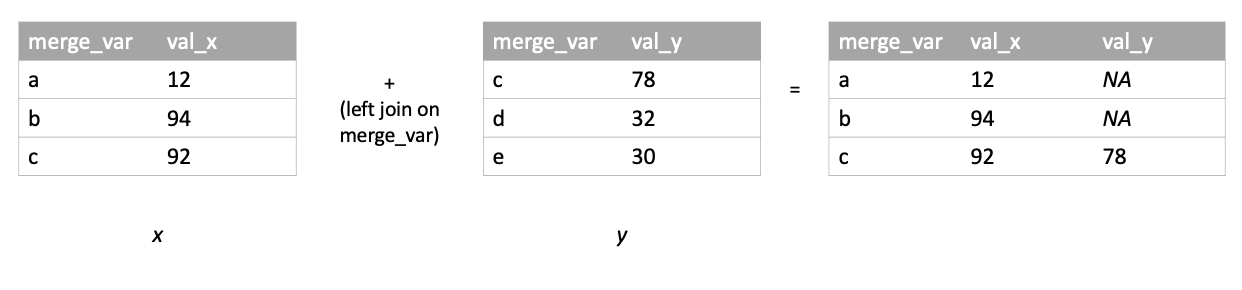
\includegraphics[width=17.25in]{images/left_join}

\hypertarget{python-27}{%
\subsubsection*{Python}\label{python-27}}
\addcontentsline{toc}{subsubsection}{Python}

\begin{Shaded}
\begin{Highlighting}[]
\OperatorTok{\textgreater{}} \ImportTok{import}\NormalTok{ pandas }\ImportTok{as}\NormalTok{ pd}
\OperatorTok{+}\NormalTok{ pd.merge(x, y, how }\OperatorTok{=} \StringTok{\textquotesingle{}left\textquotesingle{}}\NormalTok{)}
\NormalTok{  merge\_var  val\_x  val\_y}
\DecValTok{0}\NormalTok{         a   }\FloatTok{12.0}\NormalTok{    NaN}
\DecValTok{1}\NormalTok{         b   }\FloatTok{94.0}\NormalTok{    NaN}
\DecValTok{2}\NormalTok{         c   }\FloatTok{92.0}   \FloatTok{78.0}
\end{Highlighting}
\end{Shaded}

\hypertarget{r-27}{%
\subsubsection*{R}\label{r-27}}
\addcontentsline{toc}{subsubsection}{R}

\begin{Shaded}
\begin{Highlighting}[]
\SpecialCharTok{\textgreater{}} \CommentTok{\# all.x = T results in a left join}
\ErrorTok{\textgreater{}} \FunctionTok{merge}\NormalTok{(x, y, }\AttributeTok{by =} \StringTok{\textquotesingle{}merge\_var\textquotesingle{}}\NormalTok{, }\AttributeTok{all.x =}\NormalTok{ T)}
\NormalTok{  merge\_var val\_x val\_y}
\DecValTok{1}\NormalTok{         a    }\DecValTok{12}    \ConstantTok{NA}
\DecValTok{2}\NormalTok{         b    }\DecValTok{94}    \ConstantTok{NA}
\DecValTok{3}\NormalTok{         c    }\DecValTok{92}    \DecValTok{78}
\end{Highlighting}
\end{Shaded}

\hypertarget{right-join}{%
\subsection{Right Join}\label{right-join}}

A right join of \emph{x} and \emph{y} keeps all rows of \emph{y} and merges rows of \emph{x} into \emph{y} where possible based on the merge criterion:

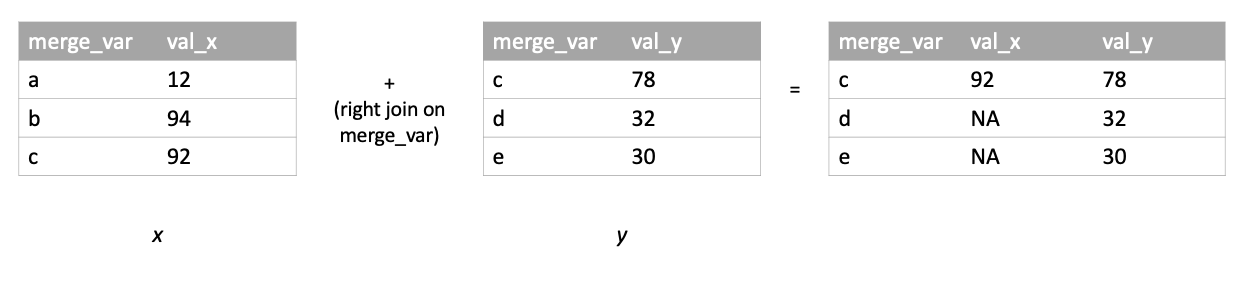
\includegraphics[width=17.25in]{images/right_join}

\hypertarget{python-28}{%
\subsubsection*{Python}\label{python-28}}
\addcontentsline{toc}{subsubsection}{Python}

\begin{Shaded}
\begin{Highlighting}[]
\OperatorTok{\textgreater{}} \ImportTok{import}\NormalTok{ pandas }\ImportTok{as}\NormalTok{ pd}
\OperatorTok{+}\NormalTok{ pd.merge(x, y, how }\OperatorTok{=} \StringTok{\textquotesingle{}right\textquotesingle{}}\NormalTok{)}
\NormalTok{  merge\_var  val\_x  val\_y}
\DecValTok{0}\NormalTok{         c   }\FloatTok{92.0}   \FloatTok{78.0}
\DecValTok{1}\NormalTok{         d    NaN   }\FloatTok{32.0}
\DecValTok{2}\NormalTok{         e    NaN   }\FloatTok{30.0}
\end{Highlighting}
\end{Shaded}

\hypertarget{r-28}{%
\subsubsection*{R}\label{r-28}}
\addcontentsline{toc}{subsubsection}{R}

\begin{Shaded}
\begin{Highlighting}[]
\SpecialCharTok{\textgreater{}} \CommentTok{\# all.y = T results in a right join}
\ErrorTok{\textgreater{}} \FunctionTok{merge}\NormalTok{(x, y, }\AttributeTok{by =} \StringTok{\textquotesingle{}merge\_var\textquotesingle{}}\NormalTok{, }\AttributeTok{all.y =}\NormalTok{ T)}
\NormalTok{  merge\_var val\_x val\_y}
\DecValTok{1}\NormalTok{         c    }\DecValTok{92}    \DecValTok{78}
\DecValTok{2}\NormalTok{         d    }\ConstantTok{NA}    \DecValTok{32}
\DecValTok{3}\NormalTok{         e    }\ConstantTok{NA}    \DecValTok{30}
\end{Highlighting}
\end{Shaded}

\hypertarget{inner-join}{%
\subsection{Inner Join}\label{inner-join}}

An inner join of \emph{x} and \emph{y} returns merged rows for which a match can be on the merge criterion \emph{in both tables}:

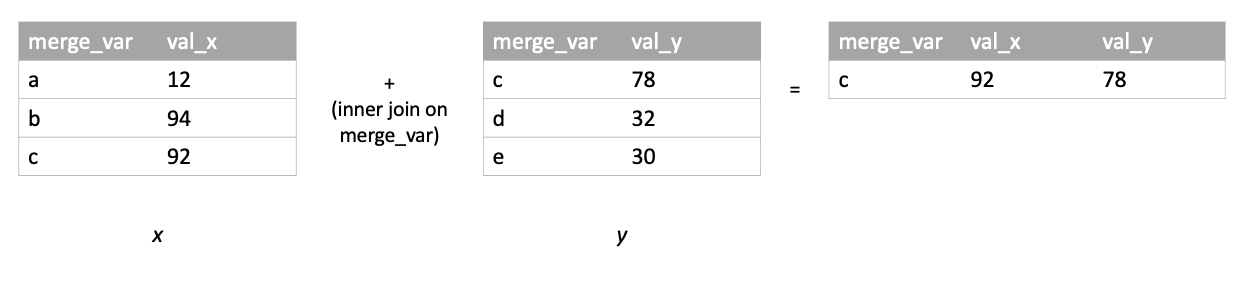
\includegraphics[width=17.25in]{images/inner_join}

\hypertarget{python-29}{%
\subsubsection*{Python}\label{python-29}}
\addcontentsline{toc}{subsubsection}{Python}

\begin{Shaded}
\begin{Highlighting}[]
\OperatorTok{\textgreater{}} \ImportTok{import}\NormalTok{ pandas }\ImportTok{as}\NormalTok{ pd}
\OperatorTok{+}\NormalTok{ pd.merge(x, y, how }\OperatorTok{=} \StringTok{\textquotesingle{}inner\textquotesingle{}}\NormalTok{)}
\NormalTok{  merge\_var  val\_x  val\_y}
\DecValTok{0}\NormalTok{         c   }\FloatTok{92.0}   \FloatTok{78.0}
\end{Highlighting}
\end{Shaded}

\hypertarget{r-29}{%
\subsubsection*{R}\label{r-29}}
\addcontentsline{toc}{subsubsection}{R}

\begin{Shaded}
\begin{Highlighting}[]
\SpecialCharTok{\textgreater{}} \CommentTok{\# by default, merge() executes an inner join}
\ErrorTok{\textgreater{}} \CommentTok{\# (more specifically, a natural join, which is a kind of}
\ErrorTok{\textgreater{}} \CommentTok{\# inner join in which the merge{-}criterion column is not}
\ErrorTok{\textgreater{}} \CommentTok{\# repeated, despite being initially present in both tables)}
\ErrorTok{\textgreater{}} \FunctionTok{merge}\NormalTok{(x, y, }\AttributeTok{by =} \StringTok{\textquotesingle{}merge\_var\textquotesingle{}}\NormalTok{)}
\NormalTok{  merge\_var val\_x val\_y}
\DecValTok{1}\NormalTok{         c    }\DecValTok{92}    \DecValTok{78}
\end{Highlighting}
\end{Shaded}

\hypertarget{outer-join}{%
\subsection{Outer Join}\label{outer-join}}

An outer join of \emph{x} and \emph{y} keeps all rows from both tables, merging rows where possible based on the merge criterion:

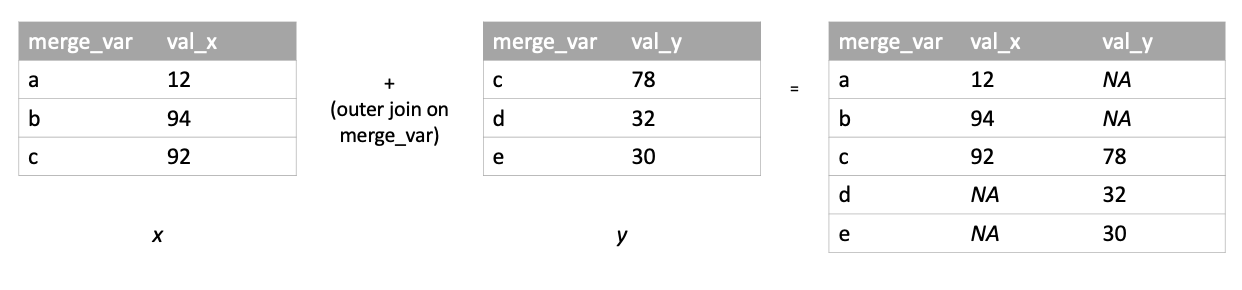
\includegraphics[width=17.25in]{images/outer_join}

\hypertarget{python-30}{%
\subsubsection*{Python}\label{python-30}}
\addcontentsline{toc}{subsubsection}{Python}

\begin{Shaded}
\begin{Highlighting}[]
\OperatorTok{\textgreater{}} \ImportTok{import}\NormalTok{ pandas }\ImportTok{as}\NormalTok{ pd}
\OperatorTok{+}\NormalTok{ pd.merge(x, y, how }\OperatorTok{=} \StringTok{\textquotesingle{}outer\textquotesingle{}}\NormalTok{)}
\NormalTok{  merge\_var  val\_x  val\_y}
\DecValTok{0}\NormalTok{         a   }\FloatTok{12.0}\NormalTok{    NaN}
\DecValTok{1}\NormalTok{         b   }\FloatTok{94.0}\NormalTok{    NaN}
\DecValTok{2}\NormalTok{         c   }\FloatTok{92.0}   \FloatTok{78.0}
\DecValTok{3}\NormalTok{         d    NaN   }\FloatTok{32.0}
\DecValTok{4}\NormalTok{         e    NaN   }\FloatTok{30.0}
\end{Highlighting}
\end{Shaded}

\hypertarget{r-30}{%
\subsubsection*{R}\label{r-30}}
\addcontentsline{toc}{subsubsection}{R}

\begin{Shaded}
\begin{Highlighting}[]
\SpecialCharTok{\textgreater{}} \CommentTok{\# all = T (or all.x = T AND all.y = T) results in an outer join}
\ErrorTok{\textgreater{}} \FunctionTok{merge}\NormalTok{(x, y, }\AttributeTok{by =} \StringTok{\textquotesingle{}merge\_var\textquotesingle{}}\NormalTok{, }\AttributeTok{all =}\NormalTok{ T)}
\NormalTok{  merge\_var val\_x val\_y}
\DecValTok{1}\NormalTok{         a    }\DecValTok{12}    \ConstantTok{NA}
\DecValTok{2}\NormalTok{         b    }\DecValTok{94}    \ConstantTok{NA}
\DecValTok{3}\NormalTok{         c    }\DecValTok{92}    \DecValTok{78}
\DecValTok{4}\NormalTok{         d    }\ConstantTok{NA}    \DecValTok{32}
\DecValTok{5}\NormalTok{         e    }\ConstantTok{NA}    \DecValTok{30}
\end{Highlighting}
\end{Shaded}

\hypertarget{aggregation-and-group-operations}{%
\chapter{Aggregation and Group Operations}\label{aggregation-and-group-operations}}

This chapter looks at manipulating and summarizing data by groups.

\hypertarget{cross-tabulation}{%
\section{Cross tabulation}\label{cross-tabulation}}

Cross tabulation is the process of determining frequencies per group (or values based on frequencies, like proportions), with groups delineated by one or more variables (e.g., nationality and sex).

The Python and R examples of cross tabulation below both make use of the following dataset, \texttt{dat}:

\begin{Shaded}
\begin{Highlighting}[]
\SpecialCharTok{\textgreater{}}\NormalTok{ dat}
\NormalTok{  nationality sex}
\DecValTok{1}\NormalTok{    Canadian   m}
\DecValTok{2}\NormalTok{      French   f}
\DecValTok{3}\NormalTok{      French   f}
\DecValTok{4}\NormalTok{    Egyptian   m}
\DecValTok{5}\NormalTok{    Canadian   f}
\end{Highlighting}
\end{Shaded}

\hypertarget{python-31}{%
\subsubsection*{Python}\label{python-31}}
\addcontentsline{toc}{subsubsection}{Python}

The \textbf{pandas} package contains a \texttt{crosstab()} function for cross tabulation with two or more variables. The \texttt{groupby()}, also in \textbf{pandas}, facilitates cross tabulation by one or more variables when used in combination with \texttt{count()}.

\begin{Shaded}
\begin{Highlighting}[]
\OperatorTok{\textgreater{}} \ImportTok{import}\NormalTok{ pandas }\ImportTok{as}\NormalTok{ pd}
\OperatorTok{+}\NormalTok{ pd.crosstab(dat.nationality, dat.sex)}
\NormalTok{sex          f  m}
\NormalTok{nationality      }
\NormalTok{Canadian     }\DecValTok{1}  \DecValTok{1}
\NormalTok{Egyptian     }\DecValTok{0}  \DecValTok{1}
\NormalTok{French       }\DecValTok{2}  \DecValTok{0}
\OperatorTok{\textgreater{}}\NormalTok{ dat.groupby(by }\OperatorTok{=} \StringTok{\textquotesingle{}nationality\textquotesingle{}}\NormalTok{).nationality.count()}
\NormalTok{nationality}
\NormalTok{Canadian    }\DecValTok{2}
\NormalTok{Egyptian    }\DecValTok{1}
\NormalTok{French      }\DecValTok{2}
\NormalTok{Name: nationality, dtype: int64}
\OperatorTok{\textgreater{}}\NormalTok{ dat.groupby(by }\OperatorTok{=}\NormalTok{ [}\StringTok{\textquotesingle{}nationality\textquotesingle{}}\NormalTok{, }\StringTok{\textquotesingle{}sex\textquotesingle{}}\NormalTok{]).nationality.count()}
\OperatorTok{+} \CommentTok{\# Or: dat.groupby(by = [\textquotesingle{}nationality\textquotesingle{}, \textquotesingle{}sex\textquotesingle{}]).sex.count()}
\NormalTok{nationality  sex}
\NormalTok{Canadian     f      }\DecValTok{1}
\NormalTok{             m      }\DecValTok{1}
\NormalTok{Egyptian     m      }\DecValTok{1}
\NormalTok{French       f      }\DecValTok{2}
\NormalTok{Name: nationality, dtype: int64}
\end{Highlighting}
\end{Shaded}

\hypertarget{r-31}{%
\subsubsection*{R}\label{r-31}}
\addcontentsline{toc}{subsubsection}{R}

The \texttt{table()} function performs cross tabulation in R. A user can enter a single grouping variable or enter multiple grouping variables separated by a comma(s). The \texttt{xtabs()} function also computes cross-tabs; a user enters the variables to be used for grouping in formula notation.

\begin{Shaded}
\begin{Highlighting}[]
\SpecialCharTok{\textgreater{}} \FunctionTok{table}\NormalTok{(dat}\SpecialCharTok{$}\NormalTok{nationality)}

\NormalTok{Canadian Egyptian   French }
       \DecValTok{2}        \DecValTok{1}        \DecValTok{2} 
\SpecialCharTok{\textgreater{}} \FunctionTok{table}\NormalTok{(dat}\SpecialCharTok{$}\NormalTok{nationality, dat}\SpecialCharTok{$}\NormalTok{sex)}
          
\NormalTok{           f m}
\NormalTok{  Canadian }\DecValTok{1} \DecValTok{1}
\NormalTok{  Egyptian }\DecValTok{0} \DecValTok{1}
\NormalTok{  French   }\DecValTok{2} \DecValTok{0}
\SpecialCharTok{\textgreater{}} \FunctionTok{xtabs}\NormalTok{(}\AttributeTok{formula =} \SpecialCharTok{\textasciitilde{}}\NormalTok{nationality }\SpecialCharTok{+}\NormalTok{ sex, }\AttributeTok{data =}\NormalTok{ dat)}
\NormalTok{           sex}
\NormalTok{nationality f m}
\NormalTok{   Canadian }\DecValTok{1} \DecValTok{1}
\NormalTok{   Egyptian }\DecValTok{0} \DecValTok{1}
\NormalTok{   French   }\DecValTok{2} \DecValTok{0}
\end{Highlighting}
\end{Shaded}

\hypertarget{group-summaries}{%
\section{Group summaries}\label{group-summaries}}

Computing statistical summaries per group.

\hypertarget{python-32}{%
\subsubsection*{Python}\label{python-32}}
\addcontentsline{toc}{subsubsection}{Python}

\hypertarget{r-32}{%
\subsubsection*{R}\label{r-32}}
\addcontentsline{toc}{subsubsection}{R}

The \texttt{aggregate()} function allows a user to easily generate by-group statistical summaries based on one or more grouping variables. Grouping variables can be declared as a list in the function's \texttt{by} argument. Alternatively, the grouping variables (and the variable to be summarized) can be passed to \texttt{aggregate()} in formula notation: \texttt{var\_to\_be\_aggregated\ \textasciitilde{}\ grouping\_var\_1\ +\ ...\ +\ grouping\_var\_N}. The summarizing function (e.g., \texttt{mean()}; \texttt{median()}; etc.) is declared in the \texttt{FUN} argument.

\begin{Shaded}
\begin{Highlighting}[]
\SpecialCharTok{\textgreater{}} \CommentTok{\# One grouping variable}
\ErrorTok{\textgreater{}} \CommentTok{\# Calculating mean of \textasciigrave{}mpg\textasciigrave{} in each \textasciigrave{}cyl\textasciigrave{} group}
\ErrorTok{\textgreater{}} \FunctionTok{aggregate}\NormalTok{(}\AttributeTok{x =}\NormalTok{ mtcars}\SpecialCharTok{$}\NormalTok{mpg, }
\SpecialCharTok{+}           \AttributeTok{by =} \FunctionTok{list}\NormalTok{(}\AttributeTok{cyl =}\NormalTok{ mtcars}\SpecialCharTok{$}\NormalTok{cyl), }
\SpecialCharTok{+}           \AttributeTok{FUN =} \StringTok{"mean"}\NormalTok{) }
\NormalTok{  cyl        x}
\DecValTok{1}   \DecValTok{4} \FloatTok{26.66364}
\DecValTok{2}   \DecValTok{6} \FloatTok{19.74286}
\DecValTok{3}   \DecValTok{8} \FloatTok{15.10000}
\end{Highlighting}
\end{Shaded}

Adding \texttt{drop=FALSE} ensures all combinations of levels are returned if no data exist at that combination. Below the final row is \texttt{NA} since there are no 8 cylinder cars with a ``straight'' engine (vs = 1).

\begin{Shaded}
\begin{Highlighting}[]
\SpecialCharTok{\textgreater{}} \CommentTok{\# Two or more grouping variables}
\ErrorTok{\textgreater{}} \CommentTok{\# Calculating max of \textasciigrave{}mpg\textasciigrave{} in each \textasciigrave{}cyl\textasciigrave{}*\textasciigrave{}vs\textasciigrave{} group}
\ErrorTok{\textgreater{}} \FunctionTok{aggregate}\NormalTok{(}\AttributeTok{x =}\NormalTok{ mtcars}\SpecialCharTok{$}\NormalTok{mpg, }
\SpecialCharTok{+}           \AttributeTok{by =} \FunctionTok{list}\NormalTok{(}\AttributeTok{cyl =}\NormalTok{ mtcars}\SpecialCharTok{$}\NormalTok{cyl, }\AttributeTok{vs =}\NormalTok{ mtcars}\SpecialCharTok{$}\NormalTok{vs), }
\SpecialCharTok{+}           \AttributeTok{FUN =} \StringTok{"max"}\NormalTok{, }\AttributeTok{drop =} \ConstantTok{FALSE}\NormalTok{) }
\NormalTok{  cyl vs    x}
\DecValTok{1}   \DecValTok{4}  \DecValTok{0} \FloatTok{26.0}
\DecValTok{2}   \DecValTok{6}  \DecValTok{0} \FloatTok{21.0}
\DecValTok{3}   \DecValTok{8}  \DecValTok{0} \FloatTok{19.2}
\DecValTok{4}   \DecValTok{4}  \DecValTok{1} \FloatTok{33.9}
\DecValTok{5}   \DecValTok{6}  \DecValTok{1} \FloatTok{21.4}
\DecValTok{6}   \DecValTok{8}  \DecValTok{1}   \ConstantTok{NA}
\end{Highlighting}
\end{Shaded}

\begin{Shaded}
\begin{Highlighting}[]
\SpecialCharTok{\textgreater{}} \CommentTok{\# Or, specify the variable to summarize and the grouping variables in formula notation}
\ErrorTok{\textgreater{}} \FunctionTok{aggregate}\NormalTok{(mpg }\SpecialCharTok{\textasciitilde{}}\NormalTok{ cyl, }\AttributeTok{data =}\NormalTok{ mtcars, }\AttributeTok{FUN =}\NormalTok{ mean)}
\SpecialCharTok{\textgreater{}} \FunctionTok{aggregate}\NormalTok{(mpg }\SpecialCharTok{\textasciitilde{}}\NormalTok{ cyl }\SpecialCharTok{+}\NormalTok{ vs, }\AttributeTok{data =}\NormalTok{ mtcars, }\AttributeTok{FUN =}\NormalTok{ max)}
\end{Highlighting}
\end{Shaded}

The \textbf{tidyverse} also offers a summarizing function, \texttt{summarize()} (or \texttt{summarise()}, for the Britons), which is in the \textbf{dplyr} package. After grouping a data frame/tibble (with, e.g., \textbf{dplyr}'s \texttt{group\_by()} function), a user passes it to \texttt{summarize()}, specifying in the function call how the summary statistic should be calculated.

\begin{Shaded}
\begin{Highlighting}[]
\SpecialCharTok{\textgreater{}} \FunctionTok{library}\NormalTok{(dplyr)}
\SpecialCharTok{\textgreater{}}\NormalTok{ mtcars }\SpecialCharTok{\%\textgreater{}\%} 
\SpecialCharTok{+}   \FunctionTok{group\_by}\NormalTok{(cyl, vs) }\SpecialCharTok{\%\textgreater{}\%} 
\SpecialCharTok{+}   \FunctionTok{summarize}\NormalTok{(}\AttributeTok{avg\_mpg =} \FunctionTok{mean}\NormalTok{(mpg))}
\StringTok{\textasciigrave{}}\AttributeTok{summarise()}\StringTok{\textasciigrave{}}\NormalTok{ has grouped output by }\StringTok{\textquotesingle{}cyl\textquotesingle{}}\NormalTok{. You can override using the }\StringTok{\textasciigrave{}}\AttributeTok{.groups}\StringTok{\textasciigrave{}}\NormalTok{ argument.}
\CommentTok{\# A tibble: 5 x 3}
\CommentTok{\# Groups:   cyl [3]}
\NormalTok{    cyl    vs avg\_mpg}
  \SpecialCharTok{\textless{}}\NormalTok{dbl}\SpecialCharTok{\textgreater{}} \ErrorTok{\textless{}}\NormalTok{dbl}\SpecialCharTok{\textgreater{}}   \ErrorTok{\textless{}}\NormalTok{dbl}\SpecialCharTok{\textgreater{}}
\DecValTok{1}     \DecValTok{4}     \DecValTok{0}    \DecValTok{26}  
\DecValTok{2}     \DecValTok{4}     \DecValTok{1}    \FloatTok{26.7}
\DecValTok{3}     \DecValTok{6}     \DecValTok{0}    \FloatTok{20.6}
\DecValTok{4}     \DecValTok{6}     \DecValTok{1}    \FloatTok{19.1}
\DecValTok{5}     \DecValTok{8}     \DecValTok{0}    \FloatTok{15.1}
\end{Highlighting}
\end{Shaded}

A benefit of \texttt{summarize()} is that it allows a user to specify relatively complicated summary calculations without needing to write an external function.

\begin{Shaded}
\begin{Highlighting}[]
\SpecialCharTok{\textgreater{}}\NormalTok{ mtcars }\SpecialCharTok{\%\textgreater{}\%} 
\SpecialCharTok{+}   \FunctionTok{group\_by}\NormalTok{(cyl, vs) }\SpecialCharTok{\%\textgreater{}\%} 
\SpecialCharTok{+}   \FunctionTok{summarize}\NormalTok{(}\AttributeTok{avg\_mpg =} \FunctionTok{mean}\NormalTok{(mpg),}
\SpecialCharTok{+}             \AttributeTok{complicated\_summary\_calculation =} 
\SpecialCharTok{+}               \FunctionTok{min}\NormalTok{(mpg)}\SpecialCharTok{\^{}}\FloatTok{0.5} \SpecialCharTok{*} 
\SpecialCharTok{+}               \FunctionTok{mean}\NormalTok{(wt)}\SpecialCharTok{\^{}}\FloatTok{0.5} \SpecialCharTok{+} 
\SpecialCharTok{+}               \FunctionTok{mean}\NormalTok{(disp)}\SpecialCharTok{\^{}}\NormalTok{(}\DecValTok{1}\SpecialCharTok{/}\FunctionTok{mean}\NormalTok{(hp)))}
\StringTok{\textasciigrave{}}\AttributeTok{summarise()}\StringTok{\textasciigrave{}}\NormalTok{ has grouped output by }\StringTok{\textquotesingle{}cyl\textquotesingle{}}\NormalTok{. You can override using the }\StringTok{\textasciigrave{}}\AttributeTok{.groups}\StringTok{\textasciigrave{}}\NormalTok{ argument.}
\CommentTok{\# A tibble: 5 x 4}
\CommentTok{\# Groups:   cyl [3]}
\NormalTok{    cyl    vs avg\_mpg complicated\_summary\_calculation}
  \SpecialCharTok{\textless{}}\NormalTok{dbl}\SpecialCharTok{\textgreater{}} \ErrorTok{\textless{}}\NormalTok{dbl}\SpecialCharTok{\textgreater{}}   \ErrorTok{\textless{}}\NormalTok{dbl}\SpecialCharTok{\textgreater{}}                           \ErrorTok{\textless{}}\NormalTok{dbl}\SpecialCharTok{\textgreater{}}
\DecValTok{1}     \DecValTok{4}     \DecValTok{0}    \DecValTok{26}                              \FloatTok{8.51}
\DecValTok{2}     \DecValTok{4}     \DecValTok{1}    \FloatTok{26.7}                            \FloatTok{8.07}
\DecValTok{3}     \DecValTok{6}     \DecValTok{0}    \FloatTok{20.6}                            \FloatTok{8.41}
\DecValTok{4}     \DecValTok{6}     \DecValTok{1}    \FloatTok{19.1}                            \FloatTok{8.81}
\DecValTok{5}     \DecValTok{8}     \DecValTok{0}    \FloatTok{15.1}                            \FloatTok{7.48}
\end{Highlighting}
\end{Shaded}

\hypertarget{basic-plotting-and-visualization}{%
\chapter{Basic Plotting and Visualization}\label{basic-plotting-and-visualization}}

This chapter looks at creating basic visualizations to explore and better understand data.

\hypertarget{histograms}{%
\section{Histograms}\label{histograms}}

Visualizing the distribution of numeric data.

\hypertarget{python-33}{%
\subsubsection*{Python}\label{python-33}}
\addcontentsline{toc}{subsubsection}{Python}

\hypertarget{r-33}{%
\subsubsection*{R}\label{r-33}}
\addcontentsline{toc}{subsubsection}{R}

\hypertarget{scatterplot}{%
\section{Scatterplot}\label{scatterplot}}

Visualizing the relationship between two numeric variables.

\hypertarget{python-34}{%
\subsubsection*{Python}\label{python-34}}
\addcontentsline{toc}{subsubsection}{Python}

\hypertarget{r-34}{%
\subsubsection*{R}\label{r-34}}
\addcontentsline{toc}{subsubsection}{R}

\hypertarget{statistical-inference-and-modeling}{%
\chapter{Statistical Inference and Modeling}\label{statistical-inference-and-modeling}}

This chapter looks at performing and interpreting common statistical analyses.

\hypertarget{comparing-group-means}{%
\section{Comparing group means}\label{comparing-group-means}}

Comparing the means of two or more groups to see if or how they differ. Two means can be analyzed with a t test. Three or more can be analyzed with ANOVA. Both the t test and ANOVA are special cases of a linear model.

\hypertarget{python-35}{%
\subsubsection*{Python}\label{python-35}}
\addcontentsline{toc}{subsubsection}{Python}

\hypertarget{r-35}{%
\subsubsection*{R}\label{r-35}}
\addcontentsline{toc}{subsubsection}{R}

\hypertarget{simple-linear-regression}{%
\section{Simple linear regression}\label{simple-linear-regression}}

Analyzing if or how the variability a numeric variable depends on another numeric variable.

\hypertarget{python-36}{%
\subsubsection*{Python}\label{python-36}}
\addcontentsline{toc}{subsubsection}{Python}

\hypertarget{r-36}{%
\subsubsection*{R}\label{r-36}}
\addcontentsline{toc}{subsubsection}{R}

\hypertarget{multiple-regression}{%
\section{Multiple regression}\label{multiple-regression}}

Analyzing if or how the variability a numeric variable depends on multiple numeric variables.

\hypertarget{python-37}{%
\subsubsection*{Python}\label{python-37}}
\addcontentsline{toc}{subsubsection}{Python}

\hypertarget{r-37}{%
\subsubsection*{R}\label{r-37}}
\addcontentsline{toc}{subsubsection}{R}

\hypertarget{logistic-regression}{%
\section{Logistic regression}\label{logistic-regression}}

Analyzing if or how the variability of a binary variable depends on one or more predictor variables.

\hypertarget{python-38}{%
\subsubsection*{Python}\label{python-38}}
\addcontentsline{toc}{subsubsection}{Python}

\hypertarget{r-38}{%
\subsubsection*{R}\label{r-38}}
\addcontentsline{toc}{subsubsection}{R}

  \bibliography{book.bib,packages.bib}

\end{document}
